\documentclass[11pt]{article}

\usepackage[margin=1in]{geometry}
\usepackage{graphicx}
\usepackage{setspace}
\usepackage{float}
\usepackage[tableposition=top]{caption}
\usepackage{tabularx}
\usepackage{gensymb}
\usepackage{enumitem}
\usepackage{tikz}
\usepackage{fancyvrb}
\usepackage{pgfgantt}
\usepackage{array}

\newcolumntype{Z}{>{\raggedleft\arraybackslash}X}

\usetikzlibrary{shapes,arrows,positioning}

\floatstyle{plaintop}
\restylefloat{table}

\linespread{1.15}

\setcounter{tocdepth}{4}
\setcounter{secnumdepth}{4}

\newcommand{\subsubsubsection}[1]{\paragraph{#1}\mbox{}}

\begin{document}

\pagenumbering{gobble}

\begin{titlepage}
	\centering

	{\huge University of Waterloo \\}
	{\Large Faculty of Engineering \\}
	{\Large Department of Electrical and Computer Engineering}

	\vspace{1.2in}

	{\Huge The Copper Chef}

	\vspace{1.2in}

	{\Large Group 2018.050 \\}

	\vspace{1.2in}

	{\Large Project Consultant \\}
	{\large Professor Christopher Nielsen}

	\vspace{1.2in}

	{\Large Prepared By \\}

	\begin{table}[h!]
	\centering
	\begin{tabular}{l l r}
		{\large Eric Bender} & {\large etbender@uwaterloo.ca} & {\large 20534384} \\
		{\large Shiva Ehtezazi} & {\large sehtezaz@uwaterloo.ca} & {\large 20529687} \\
		{\large Taylor Laekeman} & {\large tjlaekem@uwaterloo.ca} & {\large 20484137} \\
		{\large Christian Petri} & {\large capetri@uwaterloo.ca} & {\large 20484960} \\
		{\large Brian Truong} & {\large b3truong@uwaterloo.ca} & {\large 20528564}
	\end{tabular}
	\end{table}
\end{titlepage}

\tableofcontents
\newpage
\listoffigures
\newpage
\listoftables
\newpage

\pagenumbering{arabic}

\section{High-Level Description of Project}

This section provides a high-level description of the project that includes descriptions of its motivation and objectives, and a block diagram.

\subsection{Motivation}

Many variables affect the quality of a cooked steak, which should finish within a very narrow range of internal temperature, and with a good, even sear on each side \cite{doneness}.
If the cooking surface is too hot, the sides will burn instead of sear, and it becomes very easy to overshoot the desired internal temperature.
If the cooking temperature is too low, the sear will be imperfect, and the steak will lack the flavor contributed by the Maillard reaction.
If the steak is flipped too early or too late, the sides will not be seared evenly, and the cooking gradient through the steak will not be consistent.
For the amateur chef, or even just someone who doesn't want to devote them self to the culinary arts, the perfect steak is rare and elusive.
If the chef is trying to simultaneously prepare a range of side dishes, the problem is magnified.

If the manually cooked steak is lacking, the chef has few options to satisfy their carnivorous craving.
They could try to convince a friend to cook for them, but it’s not always possible to find somebody capable of improving on the first failed attempt.
They could go to a restaurant, but a steak from a restaurant will be much more expensive than a steak prepared at home.
Unless they are willing to devote themselves---academically or financially---to the perfect steak, the amateur will lead a sad, hungry life, lacking in succulence and flavor, and occupied instead with dry, overcooked, and generally substandard meat.

\subsection{Project Objective}

The objective of this project is to design and build a device capable of automatically cooking the perfect steak.
The user will load the device with a steak and indicate their preferred doneness.
By monitoring the characteristics of the steak, the device will determine when the steak is done and notify the user that the steak is ready.

\subsection{Block Diagram}

This section uses a block diagram to display the high-level design of The Copper Chef.

The device consists of five major subsystems:

\begin{itemize}[noitemsep, topsep=0pt, leftmargin=4em]
	\item a mechanical subsystem that manages the contact between the steak and the cooking element
	\item a sensory subsystem that monitors the relevant physical characteristics of the steak, specifically its temperature
  \item a software subsystem that controls The Copper Chef's mechanical components
  \item a power distribution subsystem that provides power to all components in the system
	\item an interface subsystem, that receives configuration from and communicates status to the user
\end{itemize}

The design of each subsystem is further explained in the following section.  
Figure 1 shows the block diagram of The Copper Chef.

\begin{figure}[H]
\centering
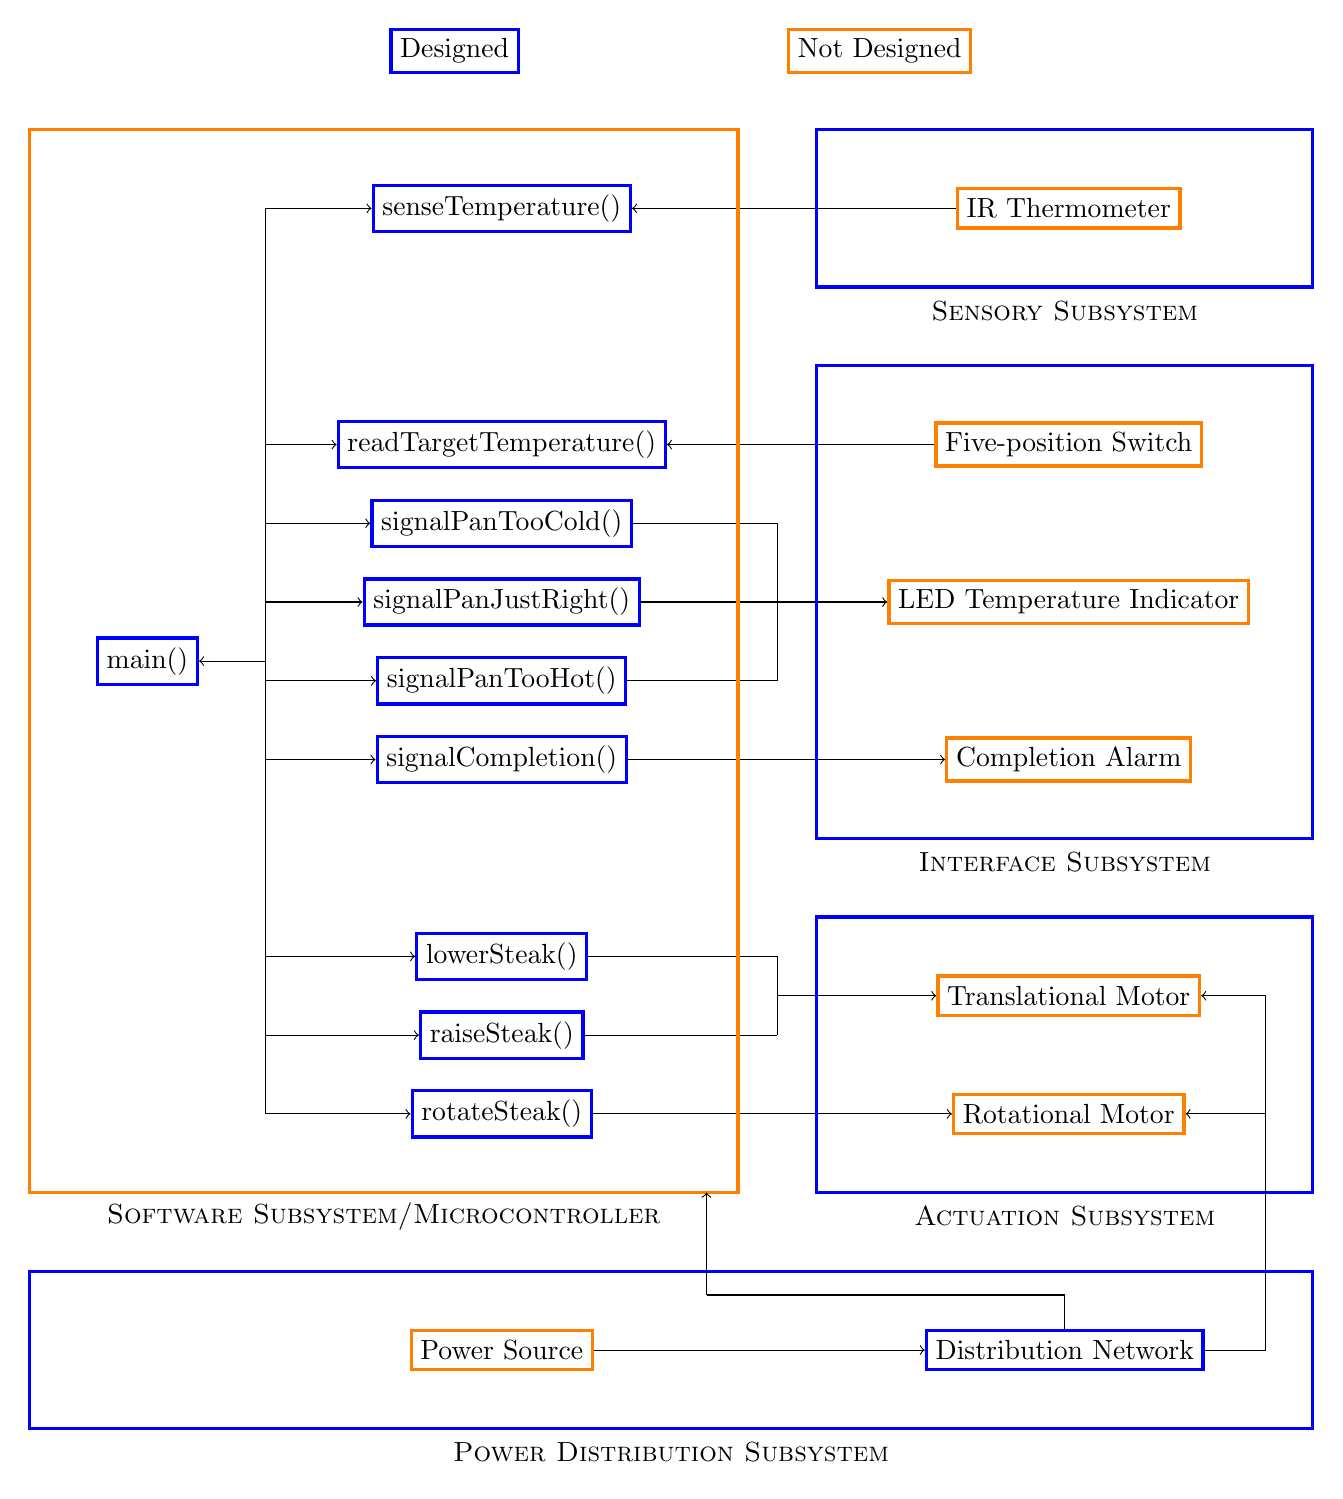
\begin{tikzpicture}[
designed/.style={rectangle, draw=blue, very thick, minimum size=5mm},
notdesigned/.style={rectangle, draw=orange, very thick, minimum size=5mm},
]

\node at (3.9,2) [designed](designed){Designed};
\node at (9.3,2) [notdesigned](notdesigned){Not Designed};

\node at (0,-5.75) [designed](main){main()};
\draw[-] (1.5,0) -- (1.5,-11.5);
\draw[<-] (main.east) -- (1.5,-5.75);

\node at (4.5,0) [designed](sense_temperature){senseTemperature()};
\node at (11.7,0) [notdesigned](thermometer){IR Thermometer};
\draw[<-] (sense_temperature.east) -- (thermometer.west);
\draw[->] (1.5,0) -- (sense_temperature.west);

\draw[blue,very thick] (8.5,1) rectangle (14.8,-1);
\node at (11.65,-1.3) {\textsc{Sensory Subsystem}};

\node at (4.5,-3) [designed](read_target_temperature){readTargetTemperature()};
\node at (11.7,-3) [notdesigned](switch){Five-position Switch};
\draw[<-] (read_target_temperature.east) -- (switch.west);
\draw[->] (1.5,-3) -- (read_target_temperature.west);

\node at (4.5,-4) [designed](too_cold){signalPanTooCold()};
\draw[->] (1.5,-4) -- (too_cold.west);
\draw[-] (too_cold.east) -- (8,-4);
\node at (4.5,-5) [designed](just_right){signalPanJustRight()};
\draw[->] (1.5,-5) -- (just_right.west);
\draw[-] (just_right.east) -- (8,-5);
\node at (4.5,-6) [designed](too_hot){signalPanTooHot()};
\draw[->] (1.5,-6) -- (too_hot.west);
\draw[-] (too_hot.east) -- (8,-6);
\node at (11.7,-5) [notdesigned](temp_led){LED Temperature Indicator};
\draw[->] (8,-5) -- (temp_led.west);
\draw[-] (8,-4) -- (8,-6);

\node at (4.5,-7) [designed](done){signalCompletion()};
\node at (11.7,-7) [notdesigned](done_bell){Completion Alarm};
\draw[->] (done.east) -- (done_bell.west);
\draw[->] (1.5,-7) -- (done.west);

\draw[blue,very thick] (8.5,-2) rectangle (14.8,-8);
\node at (11.65,-8.3) {\textsc{Interface Subsystem}};

\node at (4.5,-9.5) [designed](lower){lowerSteak()};
\draw[->] (1.5,-9.5) -- (lower.west);
\draw[-] (lower.east) -- (8,-9.5);
\node at (4.5,-10.5) [designed](raise){raiseSteak()};
\draw[->] (1.5,-10.5) -- (raise.west);
\draw[-] (raise.east) -- (8,-10.5);
\node at (11.7,-10) [notdesigned](trans){Translational Motor};
\draw[-] (8,-9.5) -- (8,-10.5);
\draw[->] (8,-10) -- (trans.west);
\draw[->] (14.2,-10) -- (trans.east);

\node at (4.5,-11.5) [designed](rotate){rotateSteak()};
\node at (11.7,-11.5) [notdesigned](rot){Rotational Motor};
\draw[->] (rotate.east) -- (rot.west);
\draw[->] (1.5,-11.5) -- (rotate.west);
\draw[->] (14.2,-11.5) -- (rot.east);

\draw[blue,very thick] (8.5,-9) rectangle (14.8,-12.5);
\node at (11.65,-12.8) {\textsc{Actuation Subsystem}};

\draw[orange,very thick] (-1.5,1) rectangle (7.5,-12.5);
\node at (3,-12.8) {\textsc{Software Subsystem/Microcontroller}};

\node at (11.65,-14.5) [designed](distribution){Distribution Network};
\node at (4.5,-14.5) [notdesigned](plug){Power Source};
\draw[->] (plug.east) -- (distribution.west);
\draw[-] (distribution.east) -- (14.2,-14.5);
\draw[-] (14.2,-10) -- (14.2,-14.5);

\draw[blue,very thick] (-1.5, -13.5) rectangle (14.8, -15.5);
\node at (6.65,-15.8) {\textsc{Power Distribution Subsystem}};

\draw[<-] (7.1,-12.5) -- (7.1,-13.8);
\draw[-] (7.1,-13.8) -- (11.65,-13.8);
\draw[-] (11.65,-13.8) -- (distribution.north);

\end{tikzpicture}
\caption{Block diagram of The Copper Chef}
\end{figure}

\section{Project Specifications}

This section presents the functional and non-functional specifications of the project.

\subsection{Functional Specifications}

Table \ref{table:func spec} shows the functional specifications of The Copper Chef.

\begin{table}[H]
\begin{tabularx}{\textwidth}{l l X}
	\hline

	Specification & Necessity & Description \\

	\hline

  Quality & Essential & The steak must be uniformly cooked, and the sides must be evenly seared. \\

	Accuracy & Essential & The internal temperature of the cooked steak must be within 1.5 \degree C of the target temperature. \\

	Autonomy & Essential & The machine must function independently, without intervention from the user. \\

	Capacity & Essential & The device must be able to cook bone-out steaks up to 1 lb (454 g) in mass. \\

  Isolation & Essential & The device must isolate the steak from the cooking surface after cooking has finished. \\

	Patience & Non-Essential & The device must hold the steak away from the heat source until it has determined that the cooking surface has reached the correct temperature. \\

	Doneness Selection & Non-Essential & The user must be allowed to select from a range of doneness options as specified by Certified Angus Beef \cite{doneness}:
  \begin{itemize}
		\item Rare (52 \degree C)
		\item Medium-Rare (57 \degree C)
		\item Medium (63 \degree C)
		\item Medium-Well (66 \degree C)
		\item Well-Done (71 \degree C)
	\end{itemize} \\ 

	Notification & Non-Essential & The user must be notified when the steak has finished cooking. \\

	\hline
\end{tabularx}
\caption{Functional specifications of The Copper Chef}
\label{table:func spec}
\end{table}

\newpage
\subsection{Non-functional Specifications}

Table \ref{table:non func spec} shows the non-functional specifications of The Copper Chef.

\begin{table}[H]
\begin{tabularx}{\textwidth}{l l X}
	\hline

	Specification & Necessity & Description \\

	\hline

	Heat Resistance & Essential & The device must be able to withstand the cooking heat to which it is exposed; components must not melt, smoke, or otherwise degrade due to the temperatures at which the device is regularly used.  \\

	Volume \& Shape & Essential & The operating dimensions of the device must be within 380 mm (width) x 330 mm (length) x 610 mm (height), where the height is measured from the flat surface on which the system sits.  These dimensions need not include the system that will interface with the external power source. \\

	Power & Essential & The device must be compatible with a typical household 15 A, 120 V receptacle. \\

	Sanitation & Non-Essential & The device must be cleanable to a level that is sufficient for its culinary application with products found in a typical kitchen. \\

	Cooking Time & Non-Essential & The device must cook a steak in at most 45 minutes, the cooking time of the Cinder, a competing automated steak-cooking system \cite{cinderprice}. \\

	Cost & Non-Essential & The device must cost less than \$ 429 USD, the cost of the Cinder \cite{cinderprice}. \\

	Weight & Non-Essential & The device must weigh less than 15 lbs (6.8 kg), the weight of a Lodge Enameled Cast Iron Dutch Oven, a heavy but frequently-moved kitchen tool \cite{lodgeweight}. \\

	\hline
\end{tabularx}
\caption{Non-functional specifications of The Copper Chef}
\label{table:non func spec}
\end{table}

\newpage
\section{Detailed Design}

The following subsections demonstrate the detailed design of The Copper Chef.

\subsection{High-Level Design}

In this section, the high-level, comprehensive design of the system is discussed.
The component subsystems of The Copper Chef are not independent, so a basic structural design that informs the specific design of each subsystem must first be established.

\subsubsection{Evaluation Criteria}

The problem has been broken down into six abstract subtasks that need to be completed.
The difficulty of each task is estimated, based on the foundation that is laid by the choice of high-level design.

Table \ref{table:high_level_criteria} shows the criteria by which the high-level designs are evaluated.

\begin{table}[H]
\begin{tabularx}{\textwidth}{X  r}

  \hline

  Criterion & Weight \\

  \hline

  Difficulty of heating the cooking element & 10 \\
  Difficulty of ensuring the heating element is the correct temperature & 10 \\
  Difficulty of placing the steak on the element & 10 \\
  Difficulty of monitoring the temperature of the steak & 10 \\
  Difficulty of ensuring the steak is cooked evenly & 10 \\
  Difficulty of removing the steak from the heat & 10 \\
  Cleanability & 20 \\
  Portability & 20 \\

  \hline

\end{tabularx}
\caption{High-level design criteria}
\label{table:high_level_criteria}
\end{table}

The difficulty estimates are equally weighted, with difficulty weighted at 60 \% overall.
The cleanability and portability of each design are also considered as stand-ins for the usability of the completed device.

Cost is not a consideration in the decision making matrix because it is extremely difficult to estimate at this high-level design stage.
It is difficult to accurately assess the cost of a device before it is clear what components will be used to build it, so an accurate estimation cannot yet be given.

\subsubsection{Overview of Candidate Designs}

Two options are being considered for the high-level design of The Copper Chef, a clamshell design that is similar to a George Foreman Grill, and a stovetop design which uses a traditional, household, stovetop range to cook the steak on a cast iron pan.

The clamshell design requires the implementation of the heating elements and the cooking surface.
It cooks both sides of the steak simultaneously, and prevents the steak from overcooking either by removing it from the heat, or reducing heat output near the completion of the cooking process.

The stovetop design specifies a device that sits on top of a consumer range that can cook a steak on a typical household frying pan, flipping it once and removing it from the heat when cooking finished.

\subsubsection{Evaluation of Designs}

The clamshell design requires the design and fabrication of a heating element upon which the steak cooks.
The stovetop design would use a regular frying pan placed on a typical consumer range or hot plate; no work needs to be done to create a heating element for the stovetop design.
The design team does not have the expertise required to design and fabricate a heated cooking surface, so the problem would require a large amount of learning, research, and trial-and-error to complete.
The stovetop design is assigned a score of zero for the difficulty of heating a cooking element, and the clamshell design is assigned a score of ten.

The device must also be confident that the heating element is the correct temperature for cooking.
Due to variation in temperatures between different consumer ranges, as well as variation in heat capacity of different frying pans, the stovetop design requires implementation of a thermometer or temperature sensor to achieve this confidence.
Since the properties of the heating element of the clamshell design are completely under the control of the design team, this is not necessary for the clamshell design.
The temperature of the heating element is determined by the current that is passed through it, and can be calibrated experimentally.
The stovetop design is assigned a score of eight and the clamshell design is assigned a score of four.

Both designs need some way of placing the steak on the hot cooking element once the cooking element has reached a suitable temperature.
For the clamshell design, the steak is pushed into the open shell by a mechanical arm.
For the stovetop design, the steak is held above the pan while the pan heats up, and lowered onto the pan once it has reached an appropriate temperature.
Both of these solutions are similarly difficult, since they each involve a simple mechanical system that must move in one direction to reposition the steak.
Both designs are assigned scores of six.

Monitoring the temperature of the steak as it being cooked is very difficult under the clamshell design.
Since the clamshell design sandwiches the steak between two hot cooking elements, the steak is largely unavailable for measurement.
A meat thermometer could be used to measure the steak’s temperature through its side, but it is difficult to guarantee that the thermometer is appropriately located to give a reading that accurately represents the internal temperature of the steak.
Alternatively, the shell could be opened and more easily measured, but this could result in uneven cooking, since one of the heating elements is not in contact with the steak while the measurement is taking place.
On the other hand, a simple IR thermometer could be used to measure the steak’s surface temperature from above in the stovetop design.
The stovetop design is assigned a score of three and the clamshell design is assigned a score of ten.

Ensuring the steak cooks evenly is more difficult with the stovetop design because the steak is only being heated from one side at a time.
This means that the steak must be flipped on the hot pan, which adds a considerable amount of mechanical and software complexity to the design.
On the other hand, the stovetop design cooks the steak from both sides with similar heating elements, so it is easy to ensure both sides cook evenly.
The stovetop design is assigned a score of ten and the clamshell design is assigned a score of zero.

The steak ultimately needs to be removed from the heating element.
The steak could be removed from the clamshell-based design in the same way that it was originally placed there, but this could damage the steak’s sear as it is dragged across the element.
The stovetop design’s vertical motion mechanism could be used to remove it from the pan without further modification, so it receives a score of six, as it did for placing the steak on the pan in the first place.
The clamshell design is assigned a score of seven for the potential problems surrounding the sear of the steak.

Both designs pose problems for cleaning, since an electrical appliance cannot be submerged in water to be cleaned.
The stovetop design is expected to be easier to clean because the pan is separate from the device and can easily be washed in a sink, while the heating elements in the clamshell design are built right into the device.
The stovetop design is likely to have fewer components that come into contact with the steak, and less overall surface area needing to be cleaned.
The clamshell design is assigned a score of three for cleanability, and the stovetop design is assigned a score of five.

The clamshell design is likely to be smaller than the stovetop design in all three dimensions; the stovetop design must be at least as wide and deep at the base as the pan it is designed to work with, while the clamshell design can be made more compact since the cooking surface is smaller.
The clamshell design is also likely to require less vertical space than the stovetop design.
Since the stovetop design actually flips the steak, vertical space is required to ensure the necessary movement is possible.
The clamshell is likely to be heavier, however, as it includes the weight of heavy metal cooking elements.
Ultimately, neither design is particularly portable.
The clamshell design is assigned a score of five for portability, and the stovetop design is assigned a score of four.

Table \ref{table:high-level design computational decision matrix} below summarizes the values that are given above.
The S columns contain the scores that each design receives, the N columns contain normalized versions of these scores, and the W columns contain the weighted scores, the normalized score multiplied by the weight of the criterion.
This format is used for all decision making matrices in this report.

Usually negative criteria (monetary cost, for example, is better when it is lower, not higher) are represented through their reciprocal, but in the case of criteria for which a design receives a score of zero, scores are instead calculated according to Equation 1.
This occurs for the difficulty of heating a cooking element and difficulty of cooking steak evenly criteria below, and other criteria in later sections of the report.

$$ Score = Maximum \, Score - Raw \, Score \, (1) $$

\begin{table}[H]
\begin{tabularx}{\textwidth}{m{5cm} r Z Z Z Z Z Z}
  \hline

  & & \multicolumn{3}{c}{Stovetop} & \multicolumn{3}{c}{Clamshell} \\ 
  Criterion & Weight & S & N & W & S & N & W \\

  \hline

  Difficulty of heating a cooking element & 10 & 10 & 1 & 10 & 0 & 0 & 0 \\
  Difficulty of ensuring heating element is the correct temperature & 10 & $ \frac{1}{8} $ & 0.5 & 5 & $ \frac{1}{4} $ & 1 & 10 \\ 
  Difficulty of placing a steak on the element & 10 & $ \frac{1}{6} $ & 1 & 10 & $ \frac{1}{6} $ & 1 & 10 \\
  Difficulty of monitoring the temperature of the steak & 10 & $ \frac{1}{3} $ & 1 & 10 & $ \frac{1}{10} $ & 0.3 & 3 \\
  Difficulty of cooking the steak evenly & 10 & 0 & 0 & 0 & 10 & 1 & 10 \\
  Difficulty of removing the steak from the heat source & 10 & $ \frac{1}{6} $ & 1 & 10 & $ \frac{1}{7} $ & 0.86 & 8.6 \\
  Cleanability & 20 & 5 & 1 & 20 & 3 & 0.6 & 12 \\
  Portability & 20 & 4 & 0.8 & 16 & 5 & 1 & 20 \\

  \hline

  \multicolumn{5}{r}{81} & \multicolumn{3}{r}{73.6} \\

  \hline

\end{tabularx}
\caption{Computational decision matrix for the high-level design}
\label{table:high-level design computational decision matrix}
\end{table}

The stovetop design is 10 \% better than the clamshell design.

\subsection{Mechanical Subsystem}

This section outlines the mechanical subsystem of the device.
The mechanical subsystem includes all of the large physical components related to the structure of the device, the handling of the steak, and all other motions that are necessary for its operation.

\subsubsection{Vertical Motion}

This section discusses The Copper Chef’s vertical motion mechanism.
The component lifts and lowers the steak, managing its contact with the pan.

\subsubsubsection{Evaluation Criteria}

\noindent
Candidate solutions are evaluated based on their estimated hours of fabrication, maximum shipping time, cost, expected lifespan, size, weight, and required torque.
Table \ref{table:vertical_motion_criteria} shows the criteria by which the vertical motion designs are evaluated.

\begin{table}[H]
\begin{tabularx}{\textwidth}{X  r}

\hline

Criterion & Weight \\

\hline 

Estimated fabrication hours & 40 \\
Maximum shipping time & 10 \\
Cost & 20 \\
Expected lifespan & 15 \\
Weight & 15 \\

\hline

\end{tabularx}
\caption{Vertical motion design criteria}
\label{table:vertical_motion_criteria}
\end{table}

To estimate the hours required to fabricate it, each design is broken down into its requisite fabrication steps and an implementation plan is created.
Time requirements are then proposed for each step, and the times estimated for each step are summed to determine a final estimate.
This process results in more accurate and considered final estimates.
The completion of the prototype is highly prioritized by the design team; a functional device that works reasonably well is better than an incomplete device with a stronger design.

Because of the limited timeline of the project, shipping times are an important consideration in the selection of a design from among the candidates.
A design that features components that are more difficult to obtain than the components of another design is less desirable.
The score assigned to a design is the maximum shipping time from among the shipping times of its components.

The project is limited in financial resources as well as time, and so cost is important to the evaluation of the candidate designs.
The evaluation of cost is straightforward;  the cost of a design is the sum of the costs of its components.

The expected lifespan of each candidate design is difficult to estimate without prototyping and testing it, which is not feasible given the resources available to the design team.
Loose estimates are obtained either through rudimentary testing where possible, or through credible external documentation.

The Copper Chef features an essential design specification concerning its weight.
The weights of each candidate design is estimated by considering the dimensions and densities of each design’s components.

\subsubsubsection{Overview of Candidate Designs}

\noindent
Three candidate designs are considered for the system that actuates the vertical motion required to manage the contact between the steak and the pan: a threaded-rod-based design, a ball-screw-based design, and a gear-rack-based design.

Figure \ref{fig:threaded rod} below shows the threaded rod-based design.

\begin{figure}[H]
  \centering
  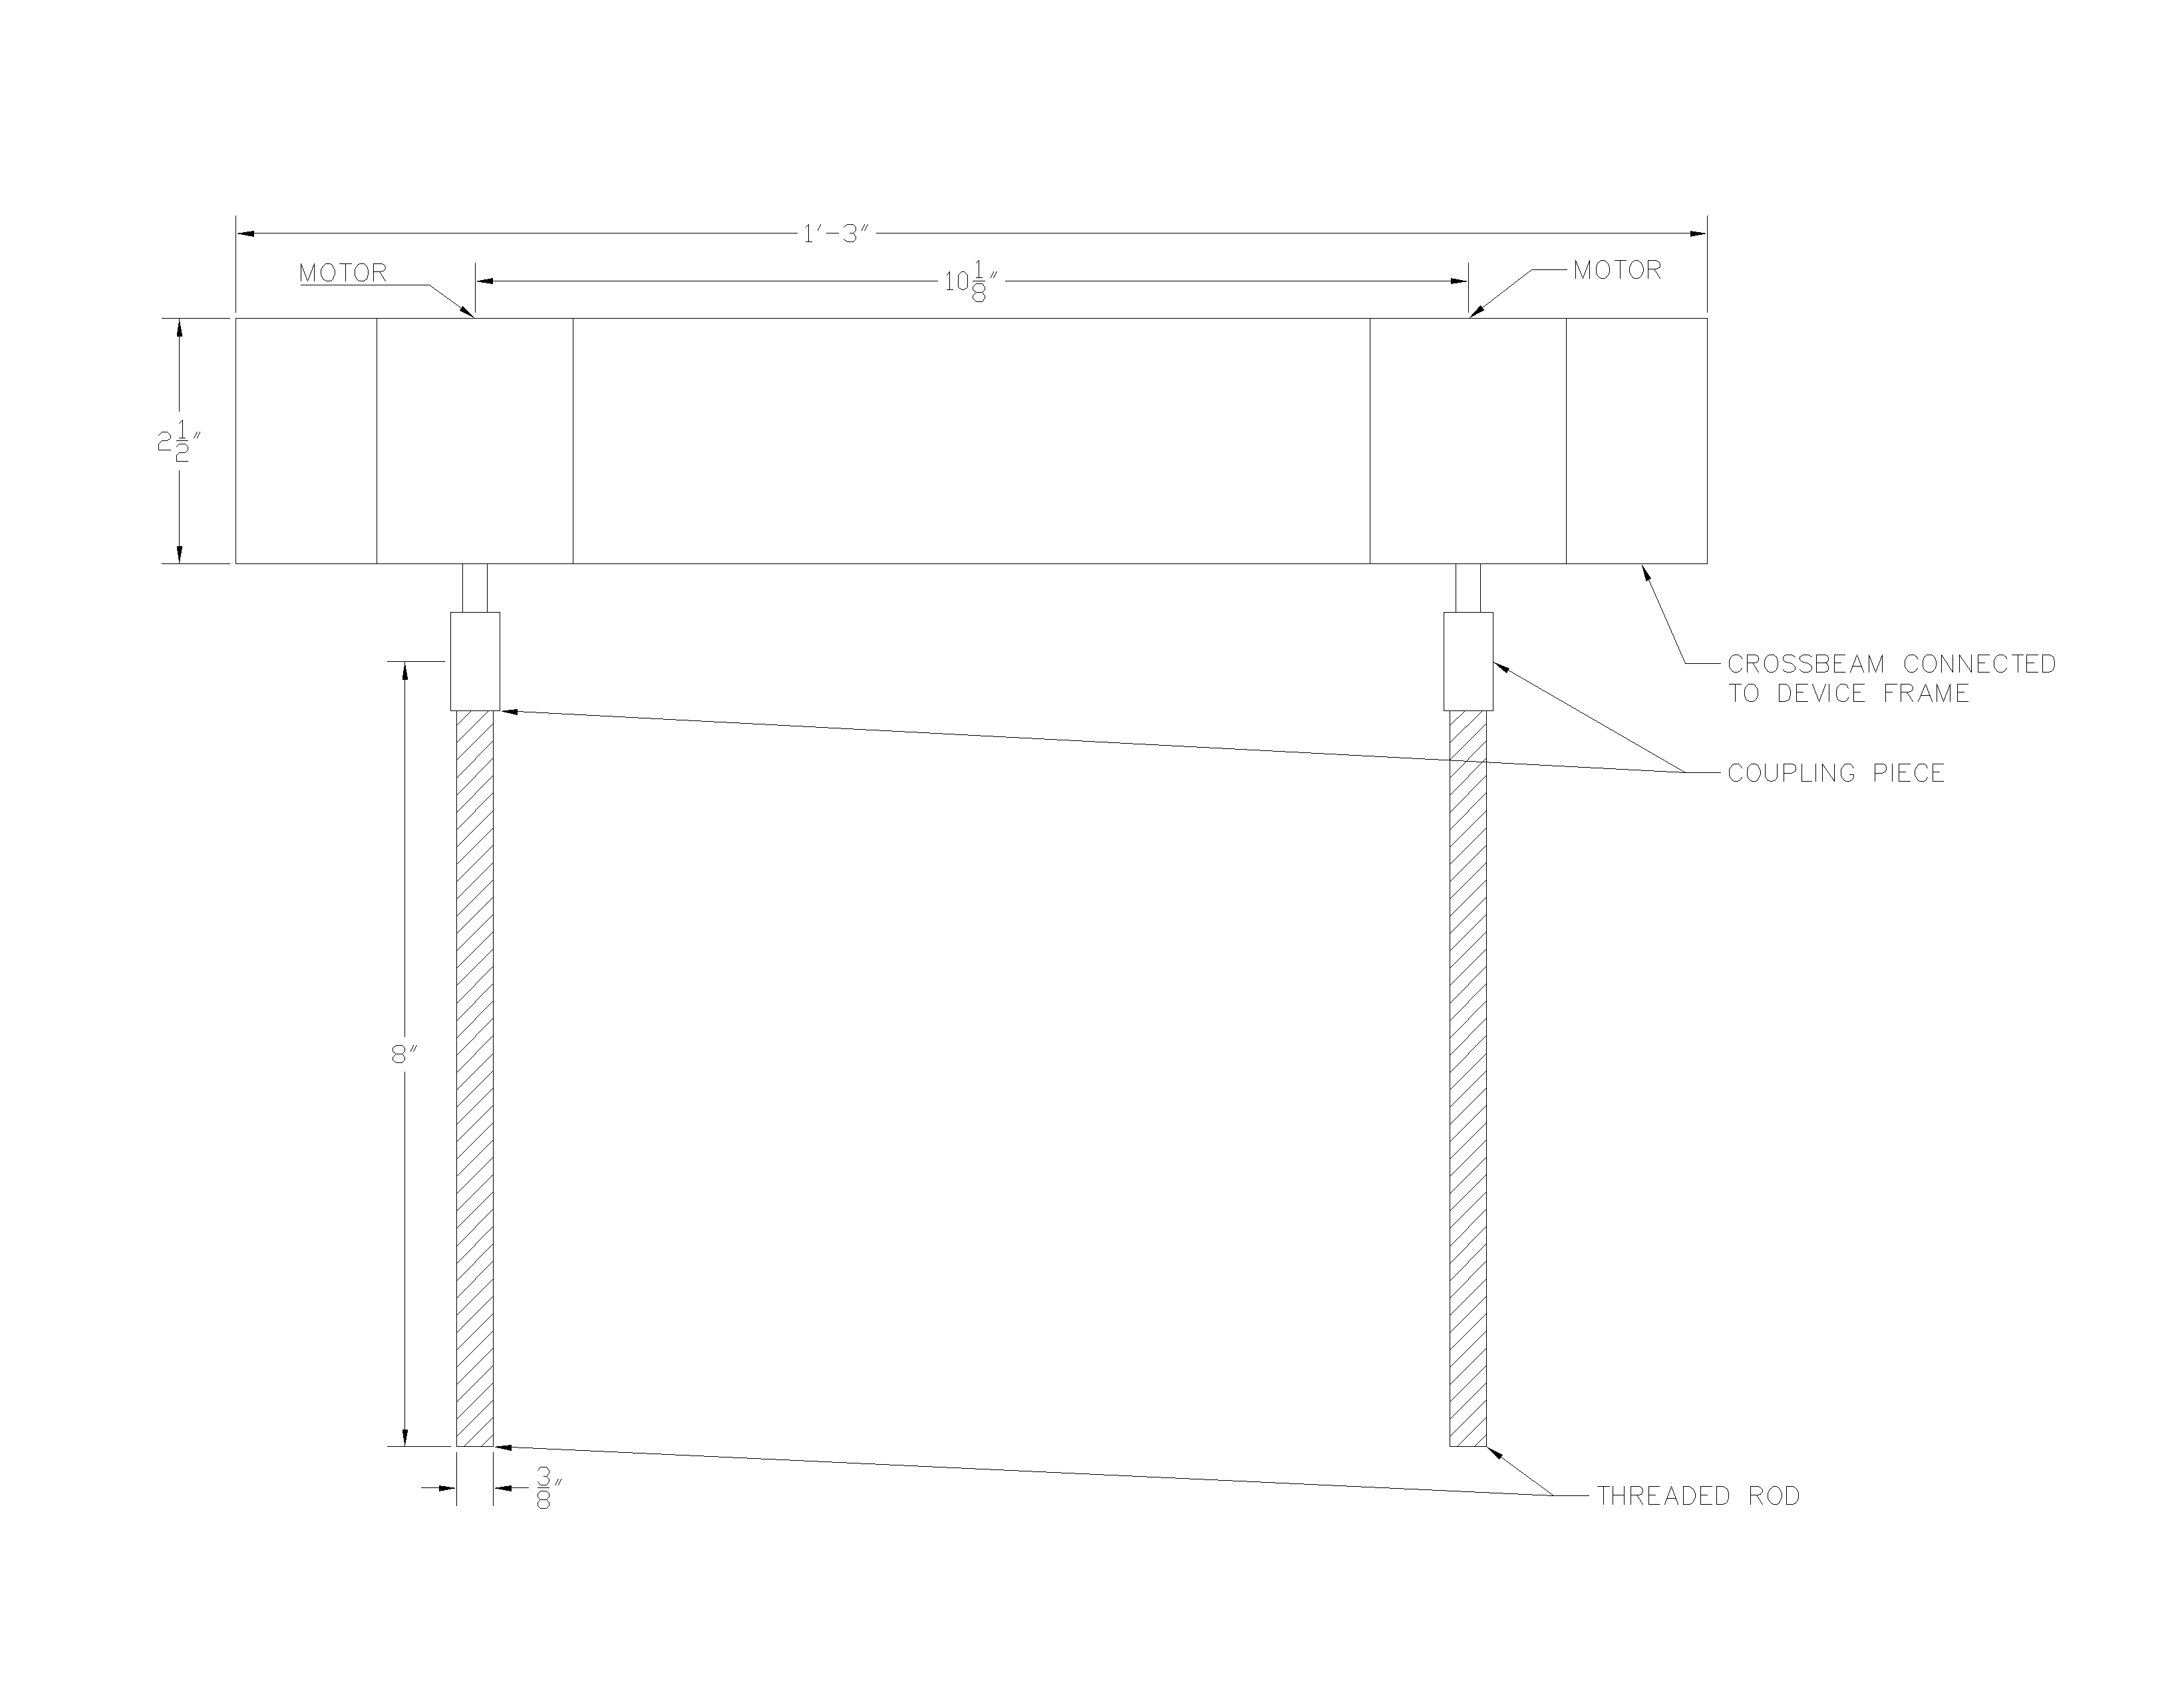
\includegraphics[width=0.6\linewidth]{res/threaded_rod.png}
  \caption{The threaded rod design}
  \label{fig:threaded rod}
\end{figure}

The two threaded rods are coupled directly to the ends of two motors, and are hung from a crossbeam attached to the frame such that the threaded rods are pointing downwards towards the pan.
A horizontal platform is screwed on to both of the threaded rods which is raised and lowered as the threaded rods turn.
This platform is not a part of the vertical motion mechanism.

Figure \ref{fig:threaded rod crossbeam} shows a detailed drawing of the crossbeam from which the motor-coupled threaded rods hang.

\begin{figure}[H]
  \centering
  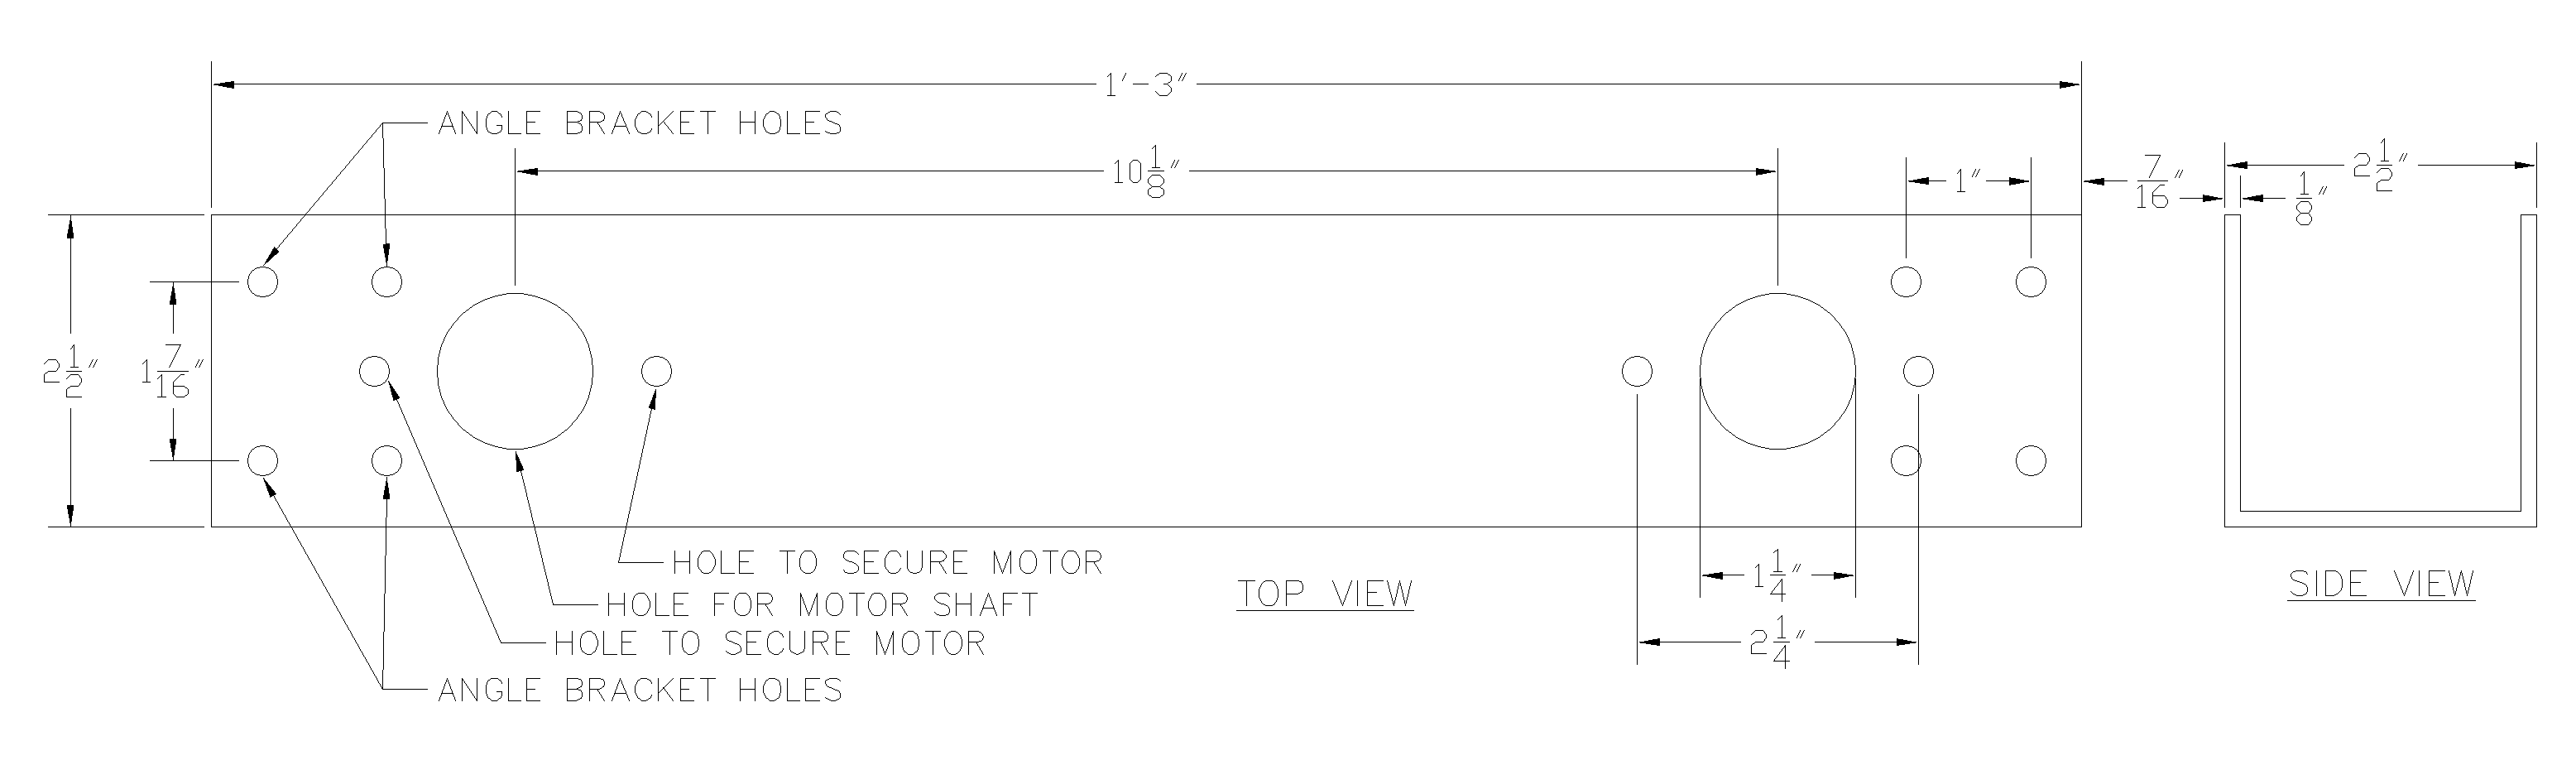
\includegraphics[width=\linewidth]{res/threaded_rod_crossbeam.png}
  \caption{The crossbeam from the threaded rod design}
  \label{fig:threaded rod crossbeam}
\end{figure}

The support is fabricated from a length of aluminum rolled-metal u bar that is fixed to the top of the frame.
The u shape greatly strengthens the crossbeam, removing the need for additional support.
The two holes at either end of the of the crossbeam are used to attach it to the frame.
Two large holes are cut into the crossbeam and the motor-coupled threaded rods are slotted into them.
Two smaller holes are drilled around the large holes, allowing the motors to be bolted to the crossbeam.

Figure \ref{fig:threaded rod coupling} shows the component that couples the motors to the threaded rods.

\begin{figure}[H]
  \centering
  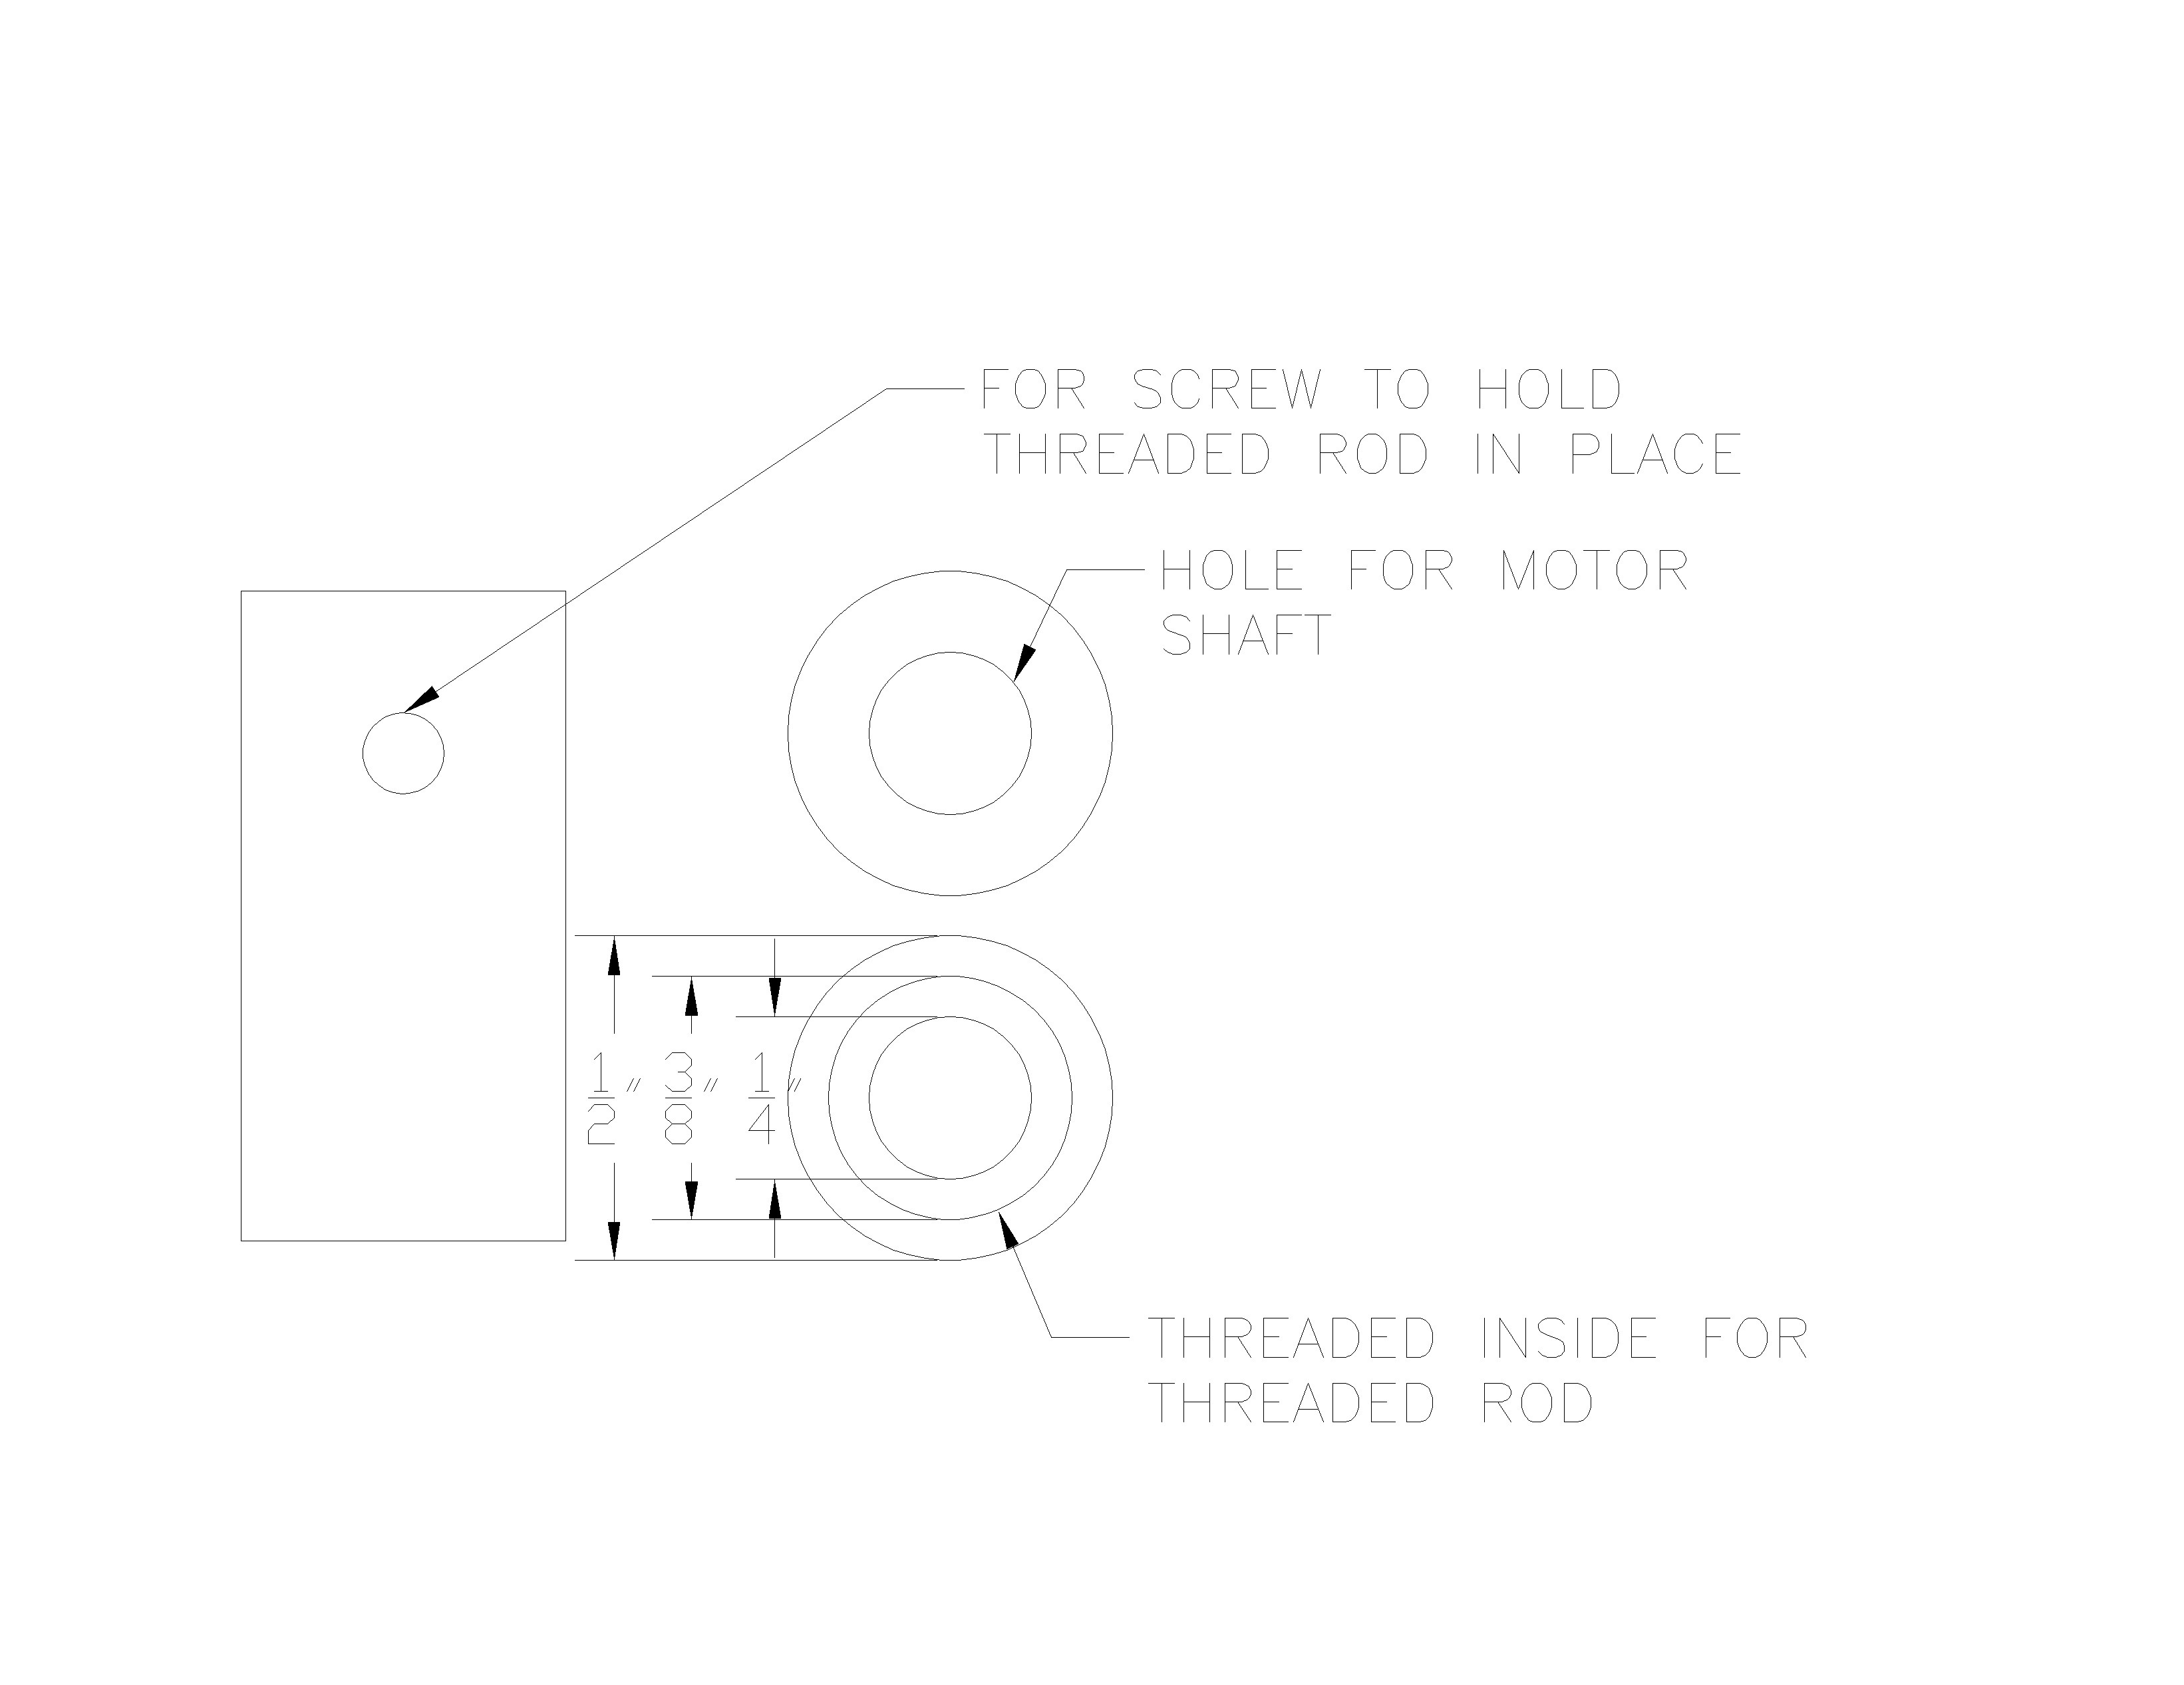
\includegraphics[width=0.6\linewidth]{res/threaded_rod_coupling.png}
  \caption{The coupling from the threaded rod design}
  \label{fig:threaded rod coupling}
\end{figure}

Two of these couplings exist in the design, one for each threaded rod and motor pair.
The couplings are short cylindrical pieces of aluminum with holes drilled axially into each end.
The shaft of a motor is fit into one of these holes, and the other is tapped and fit to a threaded rod.
A small tapped hole is drilled radially into the cylinder on the motor’s side into which a set screw is placed.
All connections to the coupling are secured with a very strong adhesive called Loctite.

The ball screw design is extremely similar to the threaded rod design.
The only differences between the two are the circumferences of the tapped holes drilled into the ends of the couplings; in one, the holes are sized to fit the threaded rods, and in the other, the ball screws.

Figure \ref{fig:gear rack} shows the candidate design that uses gear racks.

\begin{figure}[H]
  \centering
  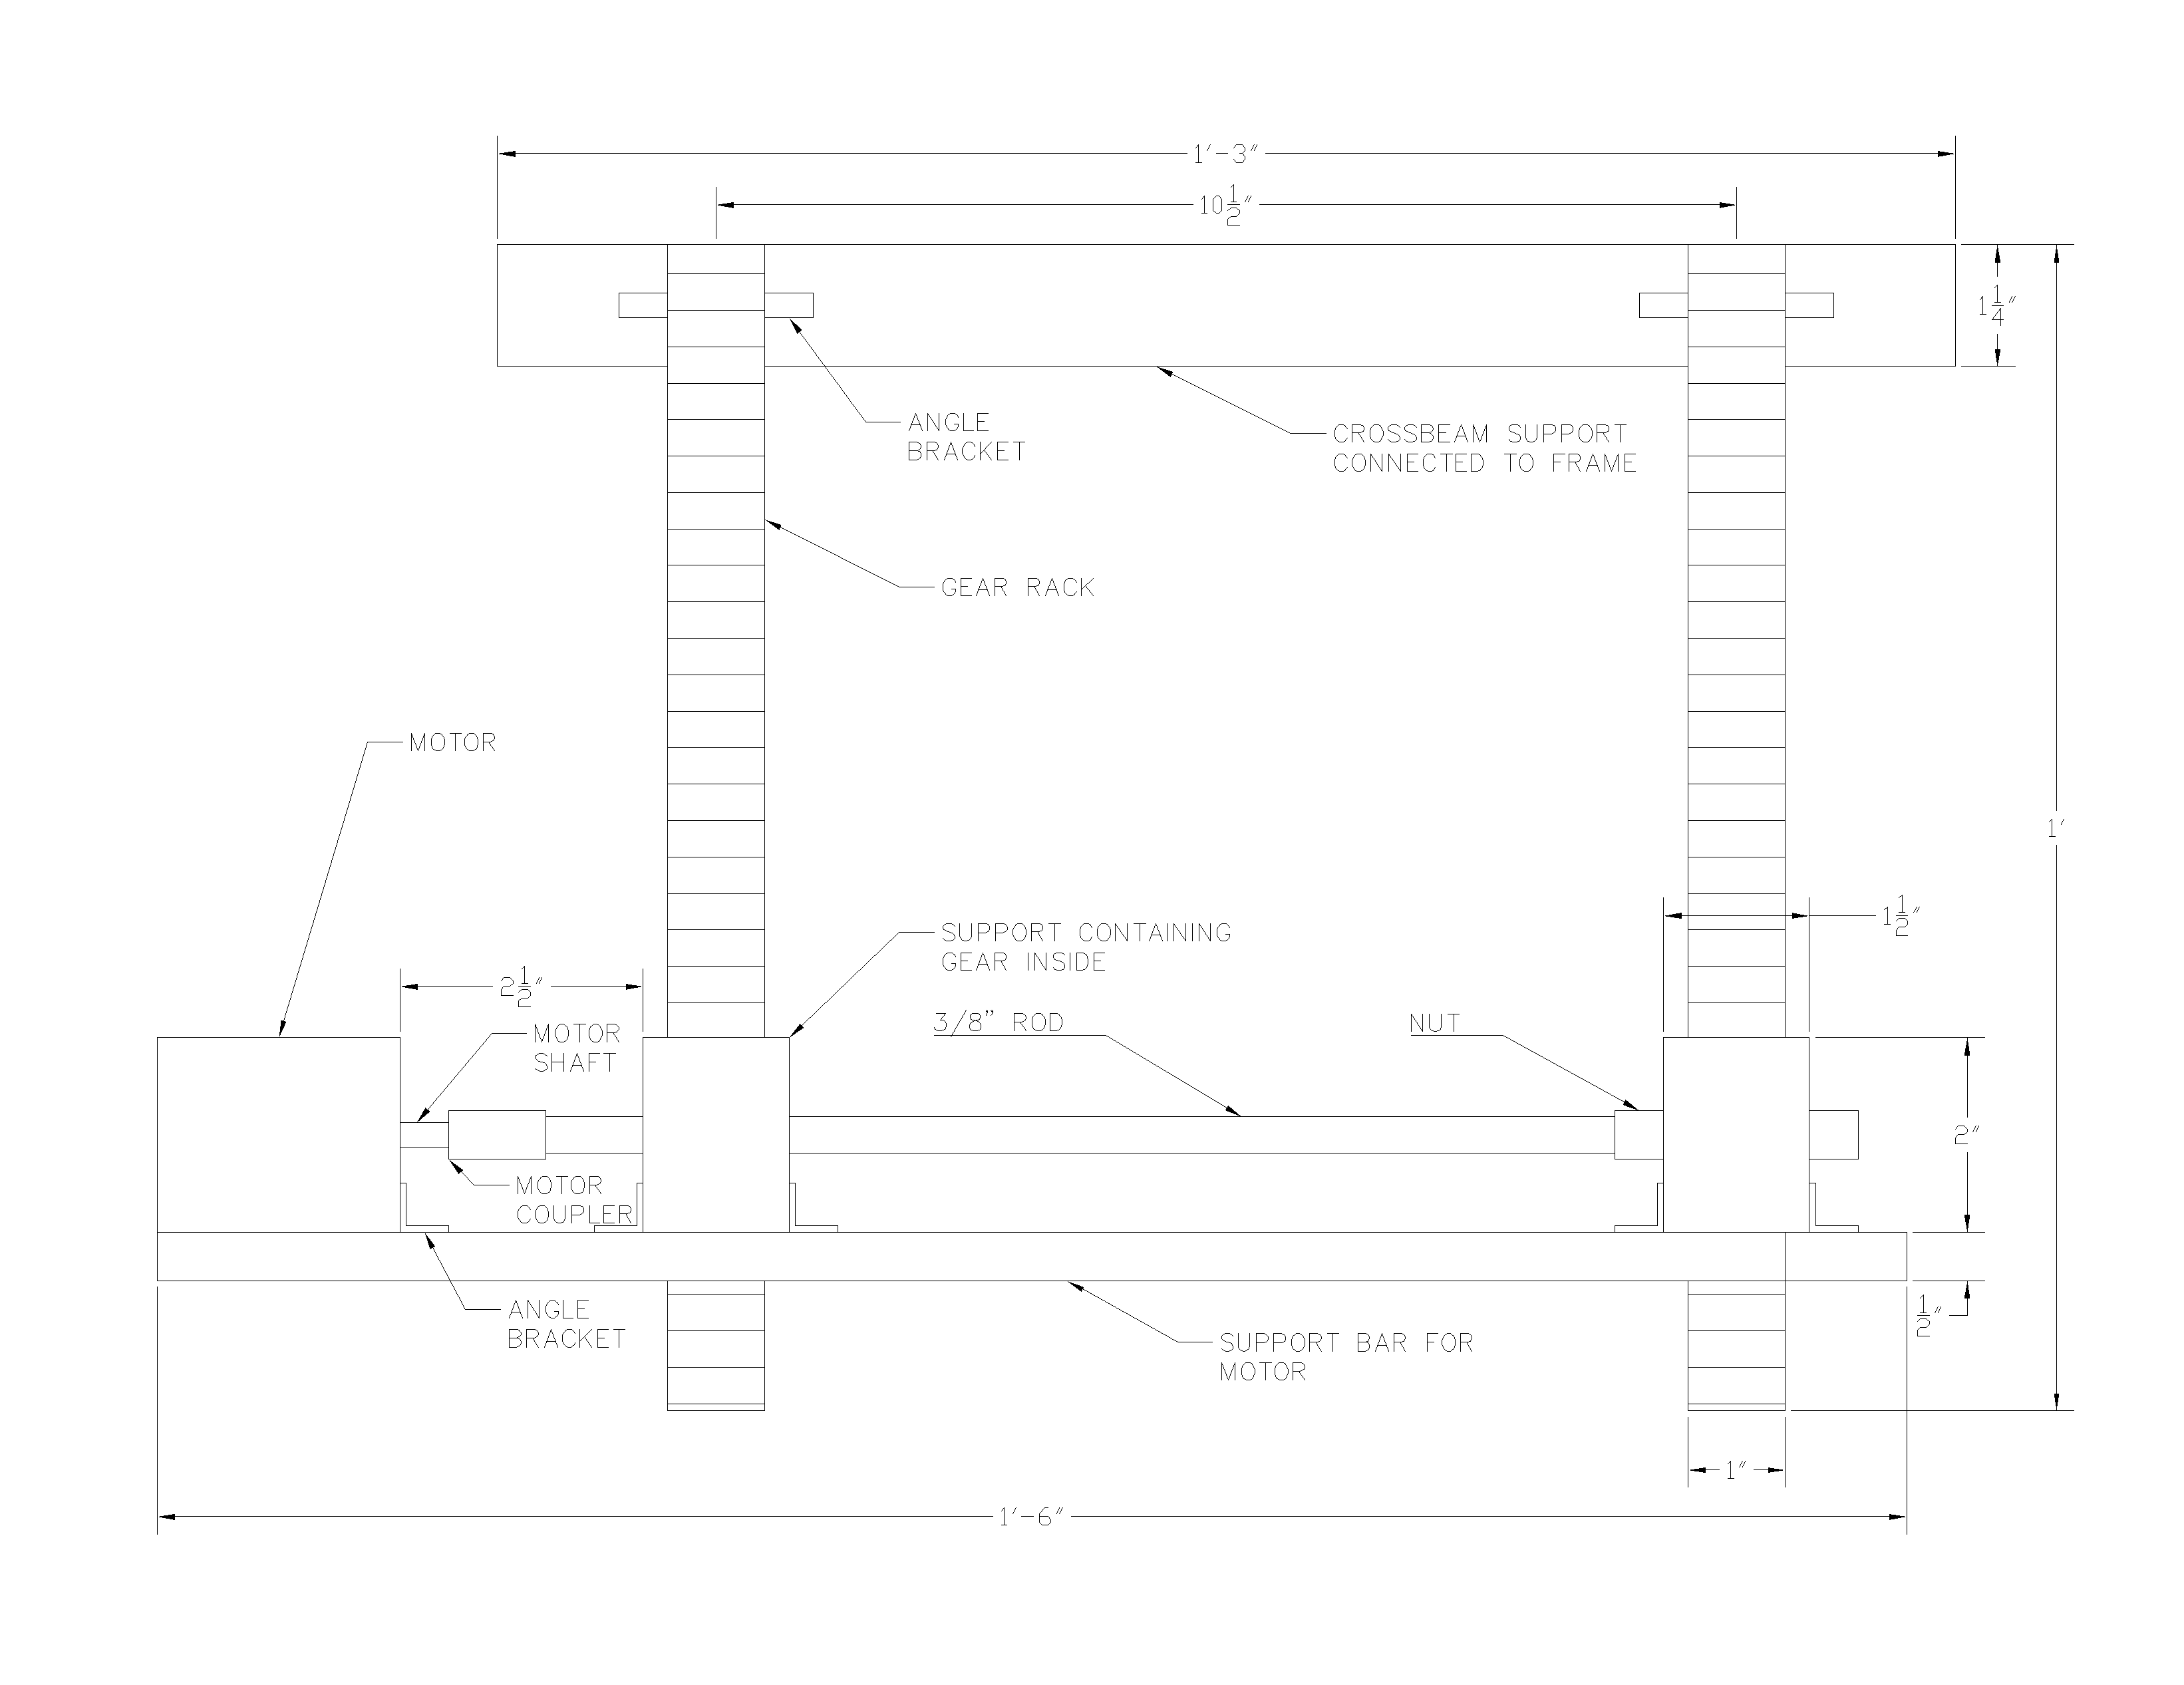
\includegraphics[width=0.6\linewidth]{res/gear_rack.png}
  \caption{The gear rack design}
  \label{fig:gear rack}
\end{figure}

Similar to the threaded rod and ball screw designs, the gear rack design features a cross beam that fixes two gear racks to the frame.
The gear racks are suspended vertically, and two gears are attached to an axle that is again coupled to a motor.
The horizontal position of these gears is fixed relative to the gear rack by a support piece that also serves to fix the orientation of the motor.
The rotational and steak-handling components of the mechanical subsystem also attach to this support piece, but they are outside of the scope of this section.

Figure \ref{fig:gear rack crossbeam} shows the details of the crossbeam.

\begin{figure}[H]
  \centering
  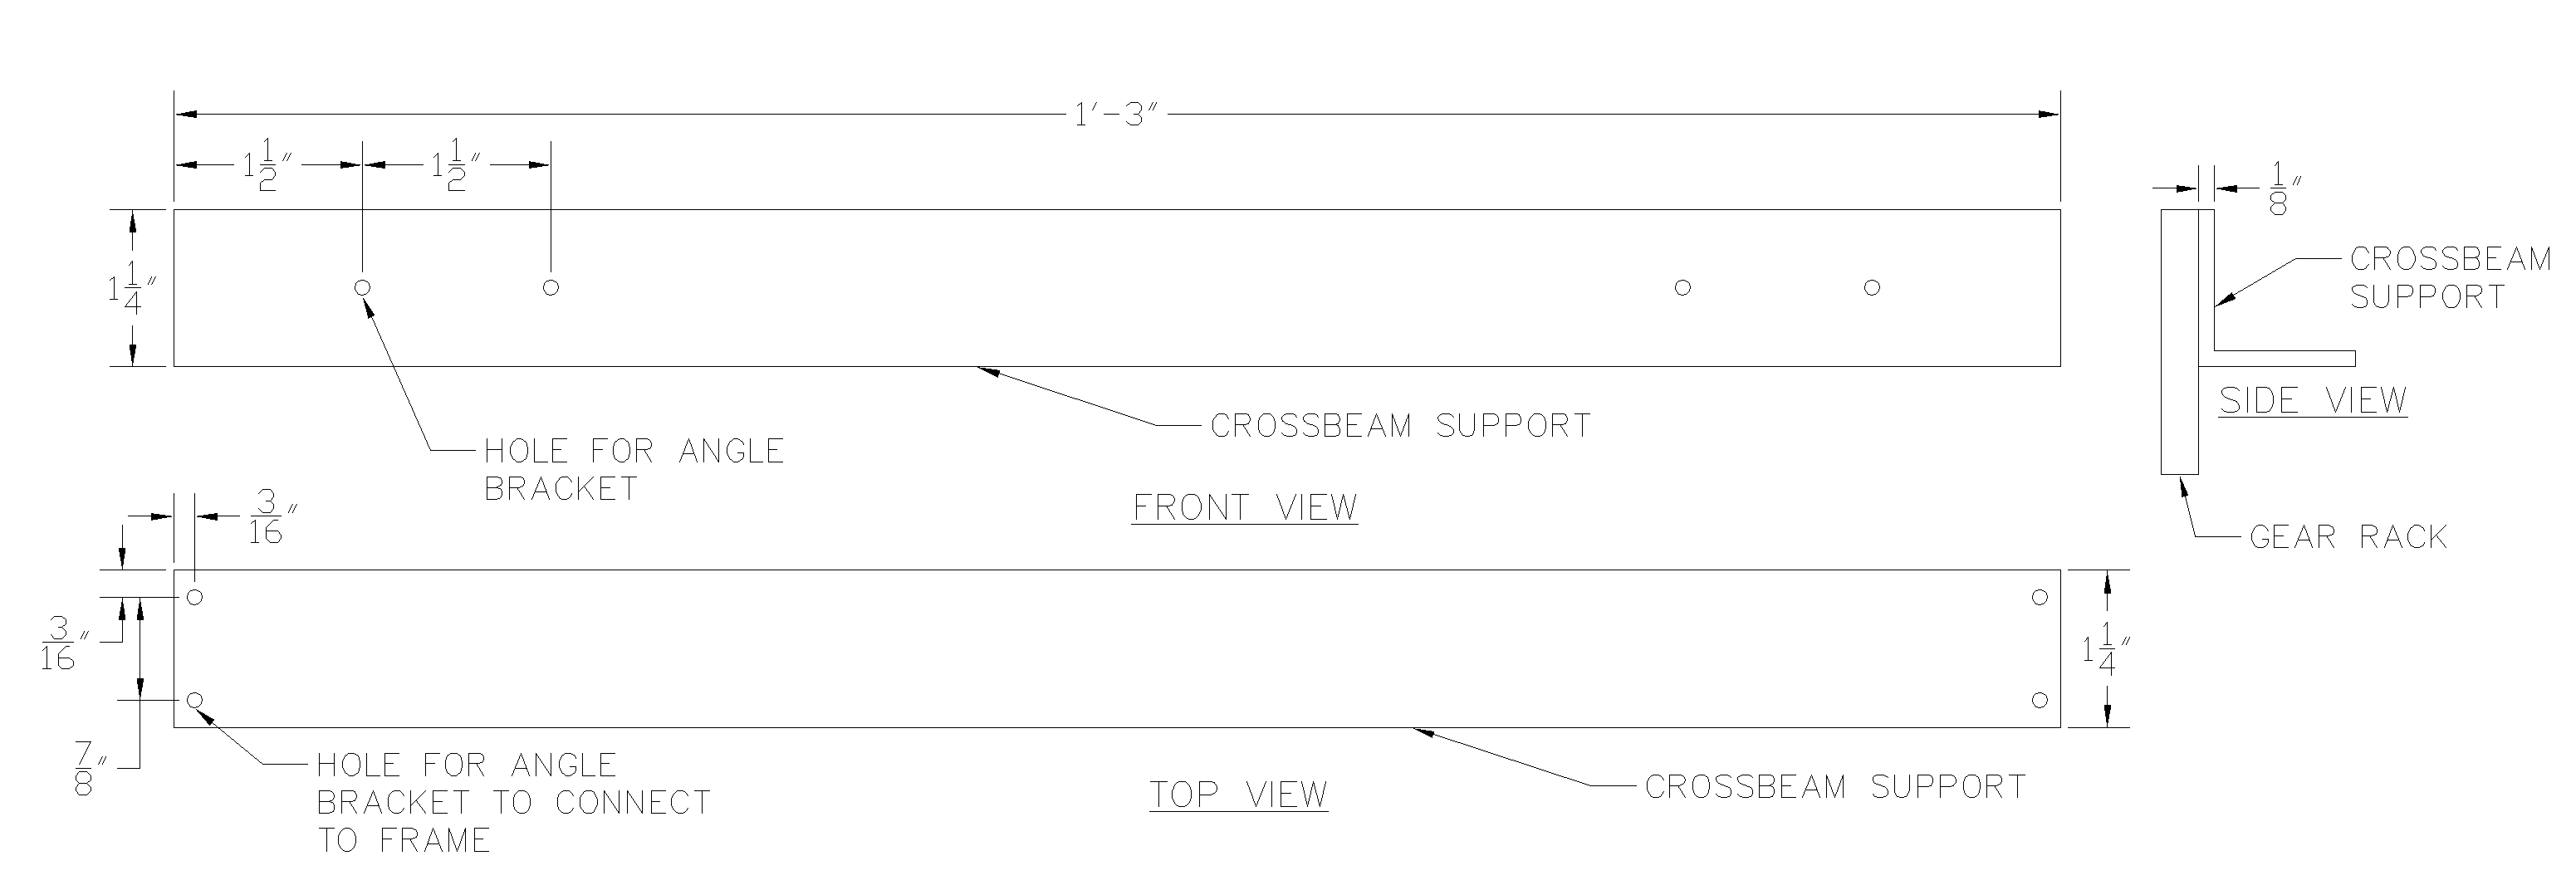
\includegraphics[width=\linewidth]{res/gear_rack_crossbeam.png}
  \caption{The crossbeam from the gear rack design}
  \label{fig:gear rack crossbeam}
\end{figure}

The gear rack’s crossbeam is an angle bar instead of the u bar used in the previous designs.
The angle provides flat surfaces to which both the frame and the gear racks are fixed.
Two holes are drilled at each end, and the beam is fixed to the frame with angle brackets.
Four holes are drilled along the length of the other face of the angle bar.
These holes are positioned so that there is one hole on each side of each gear rack.
Holes are drilled at the appropriate height on the gear rack so that they can be bolted to the crossbeam.

Figure \ref{fig:gear rack support} shows the support component in the gear rack-based design.

\begin{figure}[H]
  \centering
  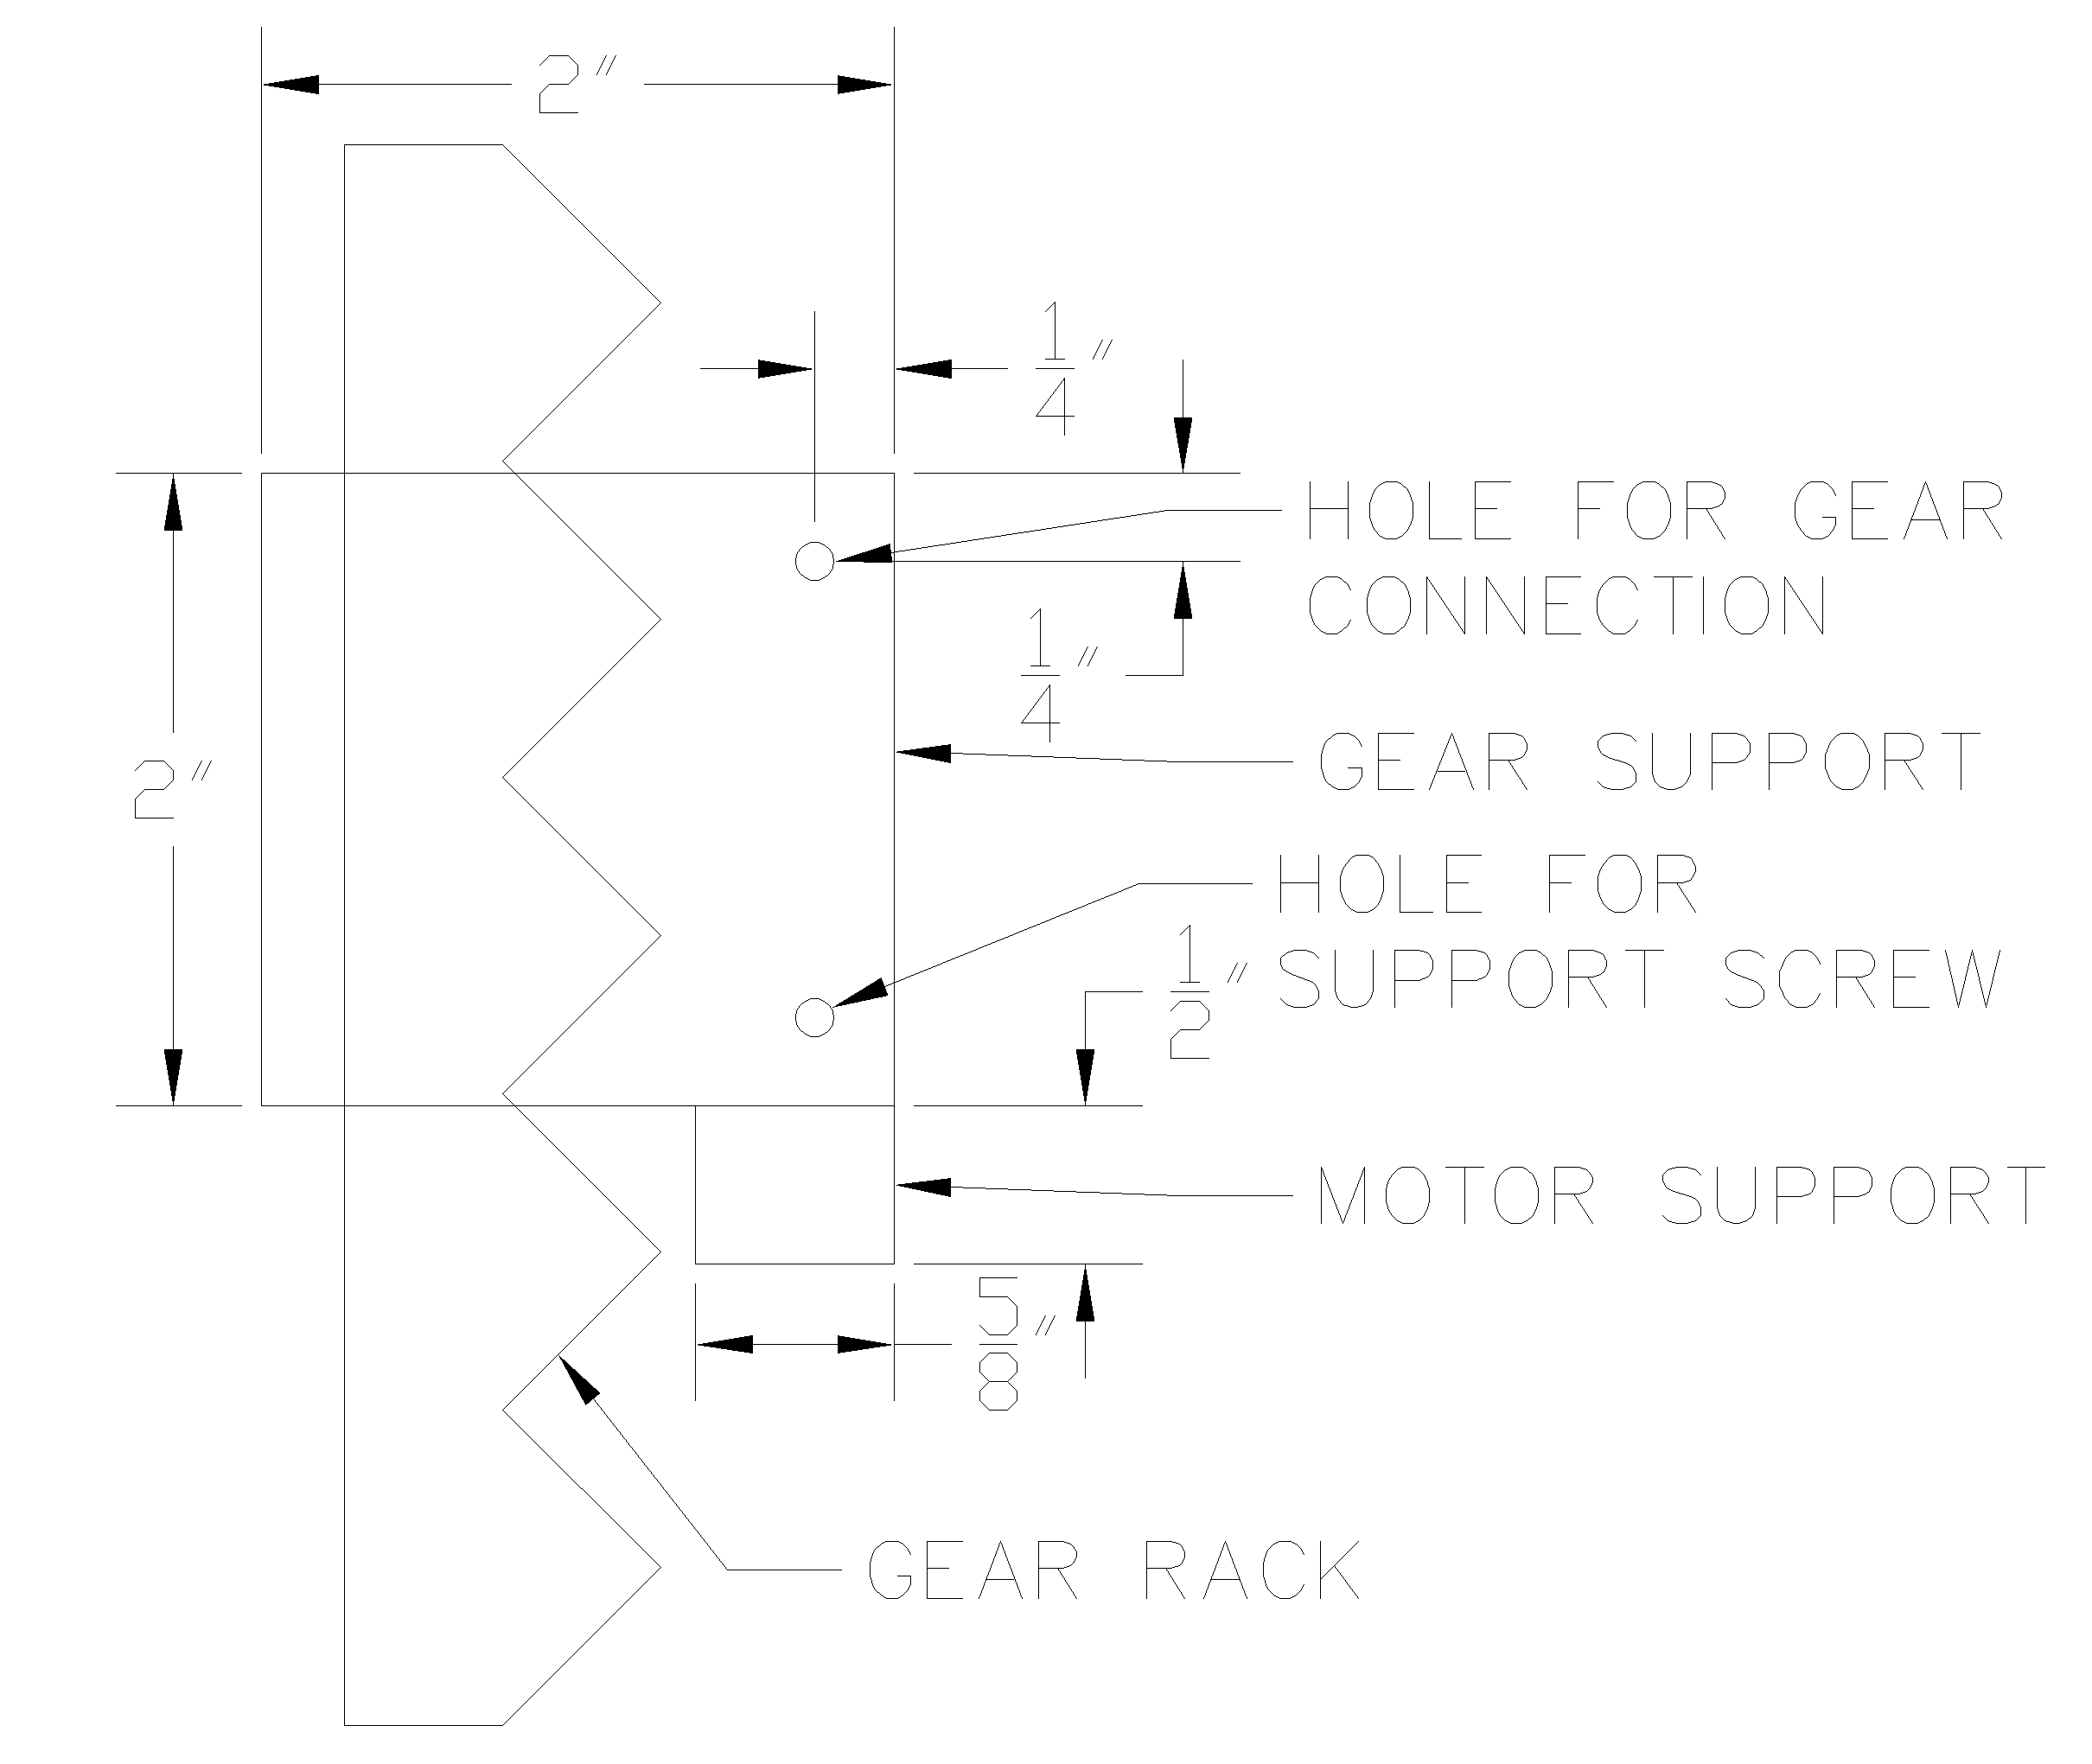
\includegraphics[width=0.4\linewidth]{res/gear_rack_support.png}
  \caption{The support component from the gear rack design}
  \label{fig:gear rack support}
\end{figure}

The support component is the most complicated piece of the gear rack design.
The gears are horizontally locked to the gear rack with a u bar.
Holes through which the axle is fed are drilled into the u bars, and two more holes are drilled below that allow the u bar to be attached to a long metal bar that runs the length of the axle.
The motor is also attached to this bar, fixing its orientation relative to the gear rack.

Figure \ref{fig:gear rack support flat bar} shows the locations of the holes drilled into the flat bar.

\begin{figure}[H]
  \centering
  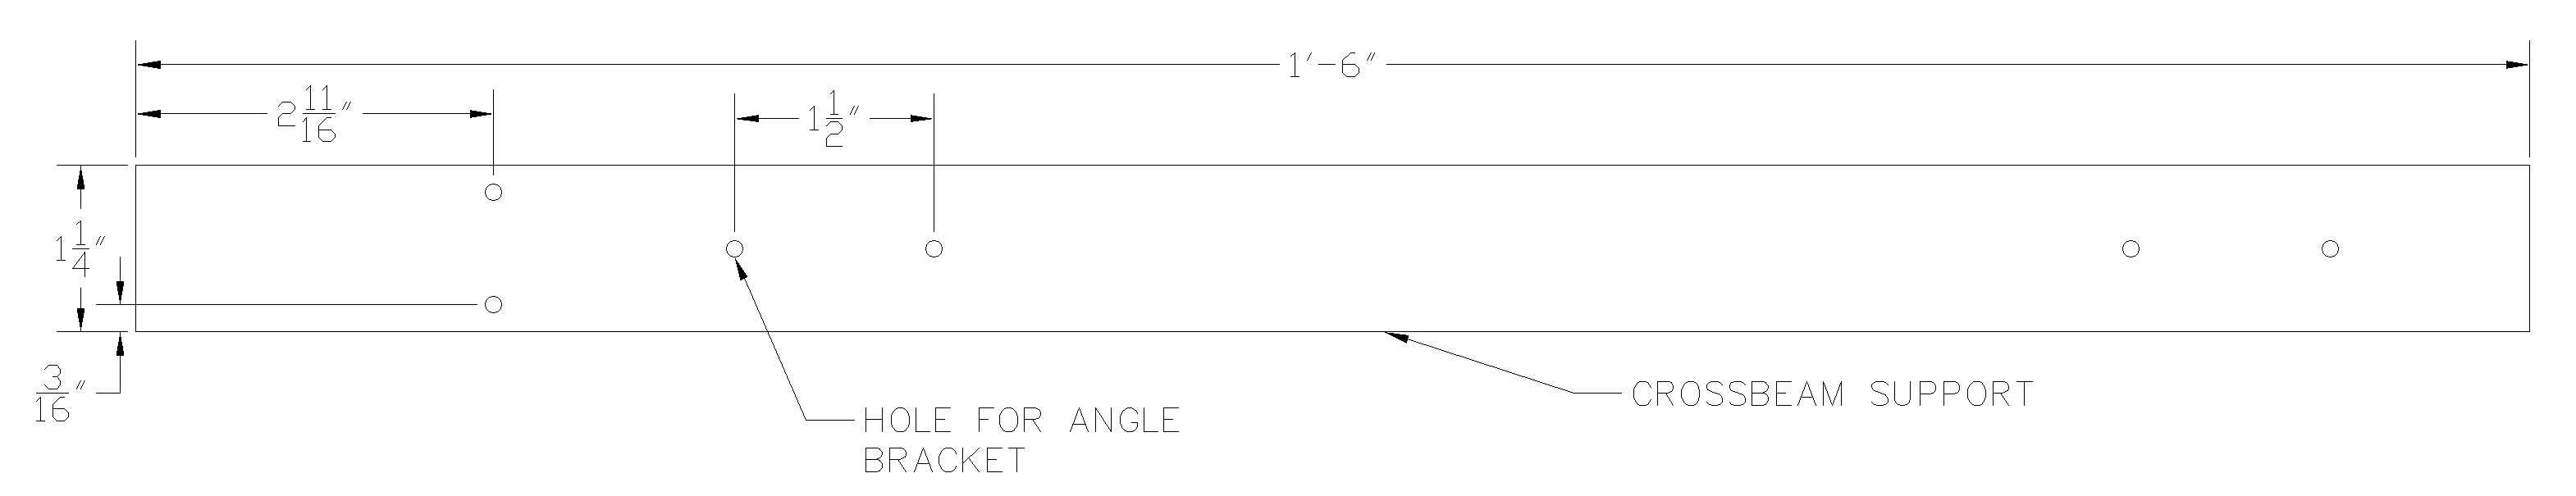
\includegraphics[width=\linewidth]{res/gear_rack_support_flat_bar.png}
  \caption{The flat bar from the support component of the gear rack design}
  \label{fig:gear rack support flat bar}
\end{figure}

Six holes are drilled into the flat bar along its length: two that allow the motors to be bolted to it, and two for each of the two u bars to be bolted to it, all with angle brackets.

\subsubsubsection{Evaluation of Designs}

Table \ref{table:vertical motion fabrication times} below shows the estimated fabrication times for the three candidate designs.  The threaded rod- and ball screw-based designs require the same work to implement, so they are estimated together.

\begin{table}[H]
\begin{tabularx}{\textwidth}{X r}

\hline

Component & Estimated Fabrication Time \\

\hline

Crossbeam & 4 \\
Coupling x 2 & 8 \\

\hline

Thread Rod, Ball Screw & 12 \\

\hline

Crossbeam & 3 \\
Coupling & 5 \\
Support U Bar x 2 & 7 \\
Support Flat Bar & 6 \\

\hline

Gear Rack & 21 \\

\hline

\end{tabularx}
\caption{Estimated fabrication times for the vertical motion mechanism}
\label{table:vertical motion fabrication times}
\end{table}

Table \ref{table:vertical motion materials} below show the costs, shipping times, and weights for the three candidate designs.

\begin{table}[H]
\begin{tabularx}{\textwidth}{l l Z Z Z Z Z}

\hline

Component & Source & Shipping Times & Cost & Volume ($ m^3 $) & Density ($ \frac{kg}{m^3} $) & Mass (kg) \\ \hline

Aluminium U Bar & Engineering Machine Shop & 0 & 1.12 & $ 230*10^{-6} $ & 2700 \cite{densities} & 0.62 \\
Aluminium Cylinder & Engineering Machine Shop & 0 & 0.13 & $ 26*10^{-6} $ & 2700 \cite{densities} & 0.070 \\
Threaded Rod & Engineering Machine Shop & 0 & 0.29 & $ 58*10^{-6} $ & 2700 \cite{densities} & 0.16 \\ \hline

Threaded Rod & & 0 & 1.54 & & & 0.85 \\ \hline

Aluminium U Bar & Engineering Machine Shop & 0 & 1.12 & $ 230*10^{-6} $ & 2700 \cite{densities} & 0.62 \\
Aluminium Cylinder & Engineering Machine Shop & 0 & 0.13 & $ 26*10^{-6} $ & 2700 \cite{densities} & 0.070 \\
Ball Screw & Bearings Canada \cite{ballscrew} & 5 & $ \$ 64.70 $ \cite{ballscrew} & $ 103 * 10^{-6} $ & 7800 \cite{densities} & 0.80 \\

\hline

Ball Screw & & 5 & 65.95 & & & 1.49 \\

\hline

Aluminium Angle Bar & Engineering Machine Shop & 0 & 0.18 & $ 38*10^{-6} $ & 2700 \cite{densities} & 0.10 \\
Gear Rack & McMaster-Carr & 5 & 19.81 & $ 390*10^{-6} $ & 7800 \cite{densities} & 3.0 \\
Gear * 2 & McMaster-Carr & 5 & 21.08 & $ 3.3*10^{-6} $ & 7800 \cite{densities} & 0.026 \\
Aluminium Rod & Engineering Machine Shop & 0 & 0.063 & $ 13*10^{-6} $ & 2700 \cite{densities} & 0.035 \\
Aluminium U Bar & Engineering Machine Shop & 0 & 0.077 & $ 16*10^{-6} $ & 2700 \cite{densities} & 0.043 \\
Aluminium Sheet & Engineering Machine Shop & 0 & 0.22 & $ 46*10^{-6} $ & 2700 \cite{densities} & 0.12 \\

\hline

Gear Rack & & 5 & 62.51 & & & 3.3 \\

\hline

\end{tabularx}
\caption{Material and component details for the vertical motion mechanism}
\label{table:vertical motion materials}
\end{table}

Testing performed by the design team showed that malfunctions began to occur after as few as five trials with the threaded rod-based design.
The lack of precision in fabrication of the rods themselves lead to an eventual misalignment of the two rods to the platform that they lift, despite the synchronized operation of the motors.

According to the estimation method developed by nook industries, the ball screw has an estimated lifespan of 10000 inches, which translates to approximately 2500 uses of the device [ballscrewlife].

As a gear rack is essentially two gears, one of which is unravelled and laid flat, the expected lifespan of the gear rack can be approximated by the expected lifespan of a gear.
The expected lifespan of the gear can be estimated to be 1000 uses.

Table \ref{table:vertical motion matrix} is the computational decision matrix for the vertical motion mechanism.

\begin{table}[H]
\begin{tabularx}{\textwidth}{m{5cm} r Z Z Z Z Z Z Z Z Z}
  \hline
  & & \multicolumn{3}{c}{Threaded Rods} & \multicolumn{3}{c}{Ball Screws} & \multicolumn{3}{c}{Gear Racks} \\ 
  Criterion & Weight & S & N & W & S & N & W & S & N & W \\

  \hline

  Estimated fabrication hours & 40 & $ \frac{1}{12} $ & 1 & 40 & $ \frac{1}{12} $ & 1 & 40 & $ \frac{1}{21} $ & 0.38 & 15 \\
  Shipping time & 5 & 5 & 1 & 5 & 0 & 0 & 0 & 0 & 0 & 0 \\
  Cost & 10 & $\frac{1}{1.54}$ & 1 & 10 & $\frac{1}{65.95}$ & 0.023 & 0.23 & $\frac{1}{62.51}$ & 0.025 & 0.25 \\
  Expected lifespan & 30 & 5 & 0.002 & 0.06 & 2500 & 1 & 30 & 1000 & 0.4 & 12 \\
  Weight & 15 & $\frac{1}{0.85}$ & 1 & 15 & $\frac{1}{1.49}$ & 0.57 & 8.6 & $\frac{1}{3.3}$ & 0.26 & 3.9 \\

  \hline

  \multicolumn{5}{r}{70} & \multicolumn{3}{r}{79} & \multicolumn{3}{r}{31} \\

  \hline

\end{tabularx}
\caption{Computational decision matrix for the vertical motion design}
\label{table:vertical motion matrix}
\end{table}

Based on the computational decision matrix, the ball screw-based design is 13 \% better than the threaded rod-based design and 126 \% better than the gear rack-based design.

\subsubsection{Steak Handling Apparatus}

This section discusses the component that handles the steak.
The design of this component must facilitate the placing of the steak on the pan, the removing of the steak from the pan, and the steak flipping movement.

\subsubsubsection{Evaluation Criteria}

\noindent
Candidate solutions are evaluated based on their impact on the the visual pattern of the sear that forms on the surface of the steak, the consistency with which they locate the steak in the pan, their estimated fabrication time, their maximum shipping time, their cost, and their weight.

Table \ref{table:steak handling apparatus criteria} shows the criteria by which the steak handling apparatus is evaluated.

\begin{table}[H]
\begin{tabularx}{\textwidth}{X  r}

\hline

Criterion & Weight \\

\hline

Impact on sear & 20 \\
Consistency of location of steak in pan & 15 \\
Estimated fabrication time & 25 \\
Cost & 15 \\
Shipping time & 5 \\
Weight & 10 \\
Cleanability & 10 \\

\hline

\end{tabularx}
\caption{Steak handling apparatus design criteria}
\label{table:steak handling apparatus criteria}
\end{table}

The design of the steak handling apparatus affects the sear on the surface of the steak.
A design that maintains contact with the steak and rests between it and the pan prevents the steak from developing the dark and delicious crust that is formed by direct contact with high heat.
This negatively impacts both the flavour of the steak and its visual appeal.
Each candidate starts with a score of ten, and loses a point for each distinct point of contact that exists between it and the steak.
In other words, for each visual blemish in the sear, the design loses a point.
The percentage of the surface area of the steak that is affected by the design is also estimated, and the design loses an additional point for every 10 \% that is estimated, rounded up.
A design that imparts two distinct visual blemishes and affects the sear on 12 \% of the surface of the steak loses four points, resulting in a final score of six.

A design that does not maintain contact with the steak is problematic because it introduces the potential for variability in the steak’s position and orientation.
In extreme cases, this variability could lead to malfunction when the steak is flipped.
A design receives a score of one if it maintains contact and a relative position with the steak throughout the cooking process, and a score of zero if it loses contact with the steak at any point, or if it moves independently from the steak.

Complexity is approximated through an estimate of the number of hours required to implement the design.
Estimates are made for the components or pieces of the design that need to be fabricated, and these small estimates are summed to compute a comprehensive estimate for each design.

Availability represents the time it would take to obtain the components necessary to implement a design.
The availability of the design is the maximum from the shipping times of the components, pieces, or materials that are required in the construction of the design.

As the steak handling apparatus is in direct contact with the food, it must be sanitary.
Cleanability represents the degree to which the design can be cleaned, in order to maintain safe and hygienic cooking conditions.
Cleanability is very difficult to measure without prototyping each candidate design, and taking measurements with complex and expensive machinery.
It is estimated qualitatively for this report, based on a reasoned consideration of each design.

\subsubsubsection{Overview of Candidate Designs}

\noindent
The candidate steak cooking apparatus designs are a cage-based design, featuring two tennis racket-like baskets to sandwich the steak, a spatula-based design which closely mimics the traditional, non-automated method of steak cooking on a stovetop, and a design that is similar to the cage-based design, but features a thin metallic mesh in place of the tennis racket-like wiring.

Figure \ref{fig:cage} shows a comprehensive view of the cage-based design.

\begin{figure}[H]
  \centering
  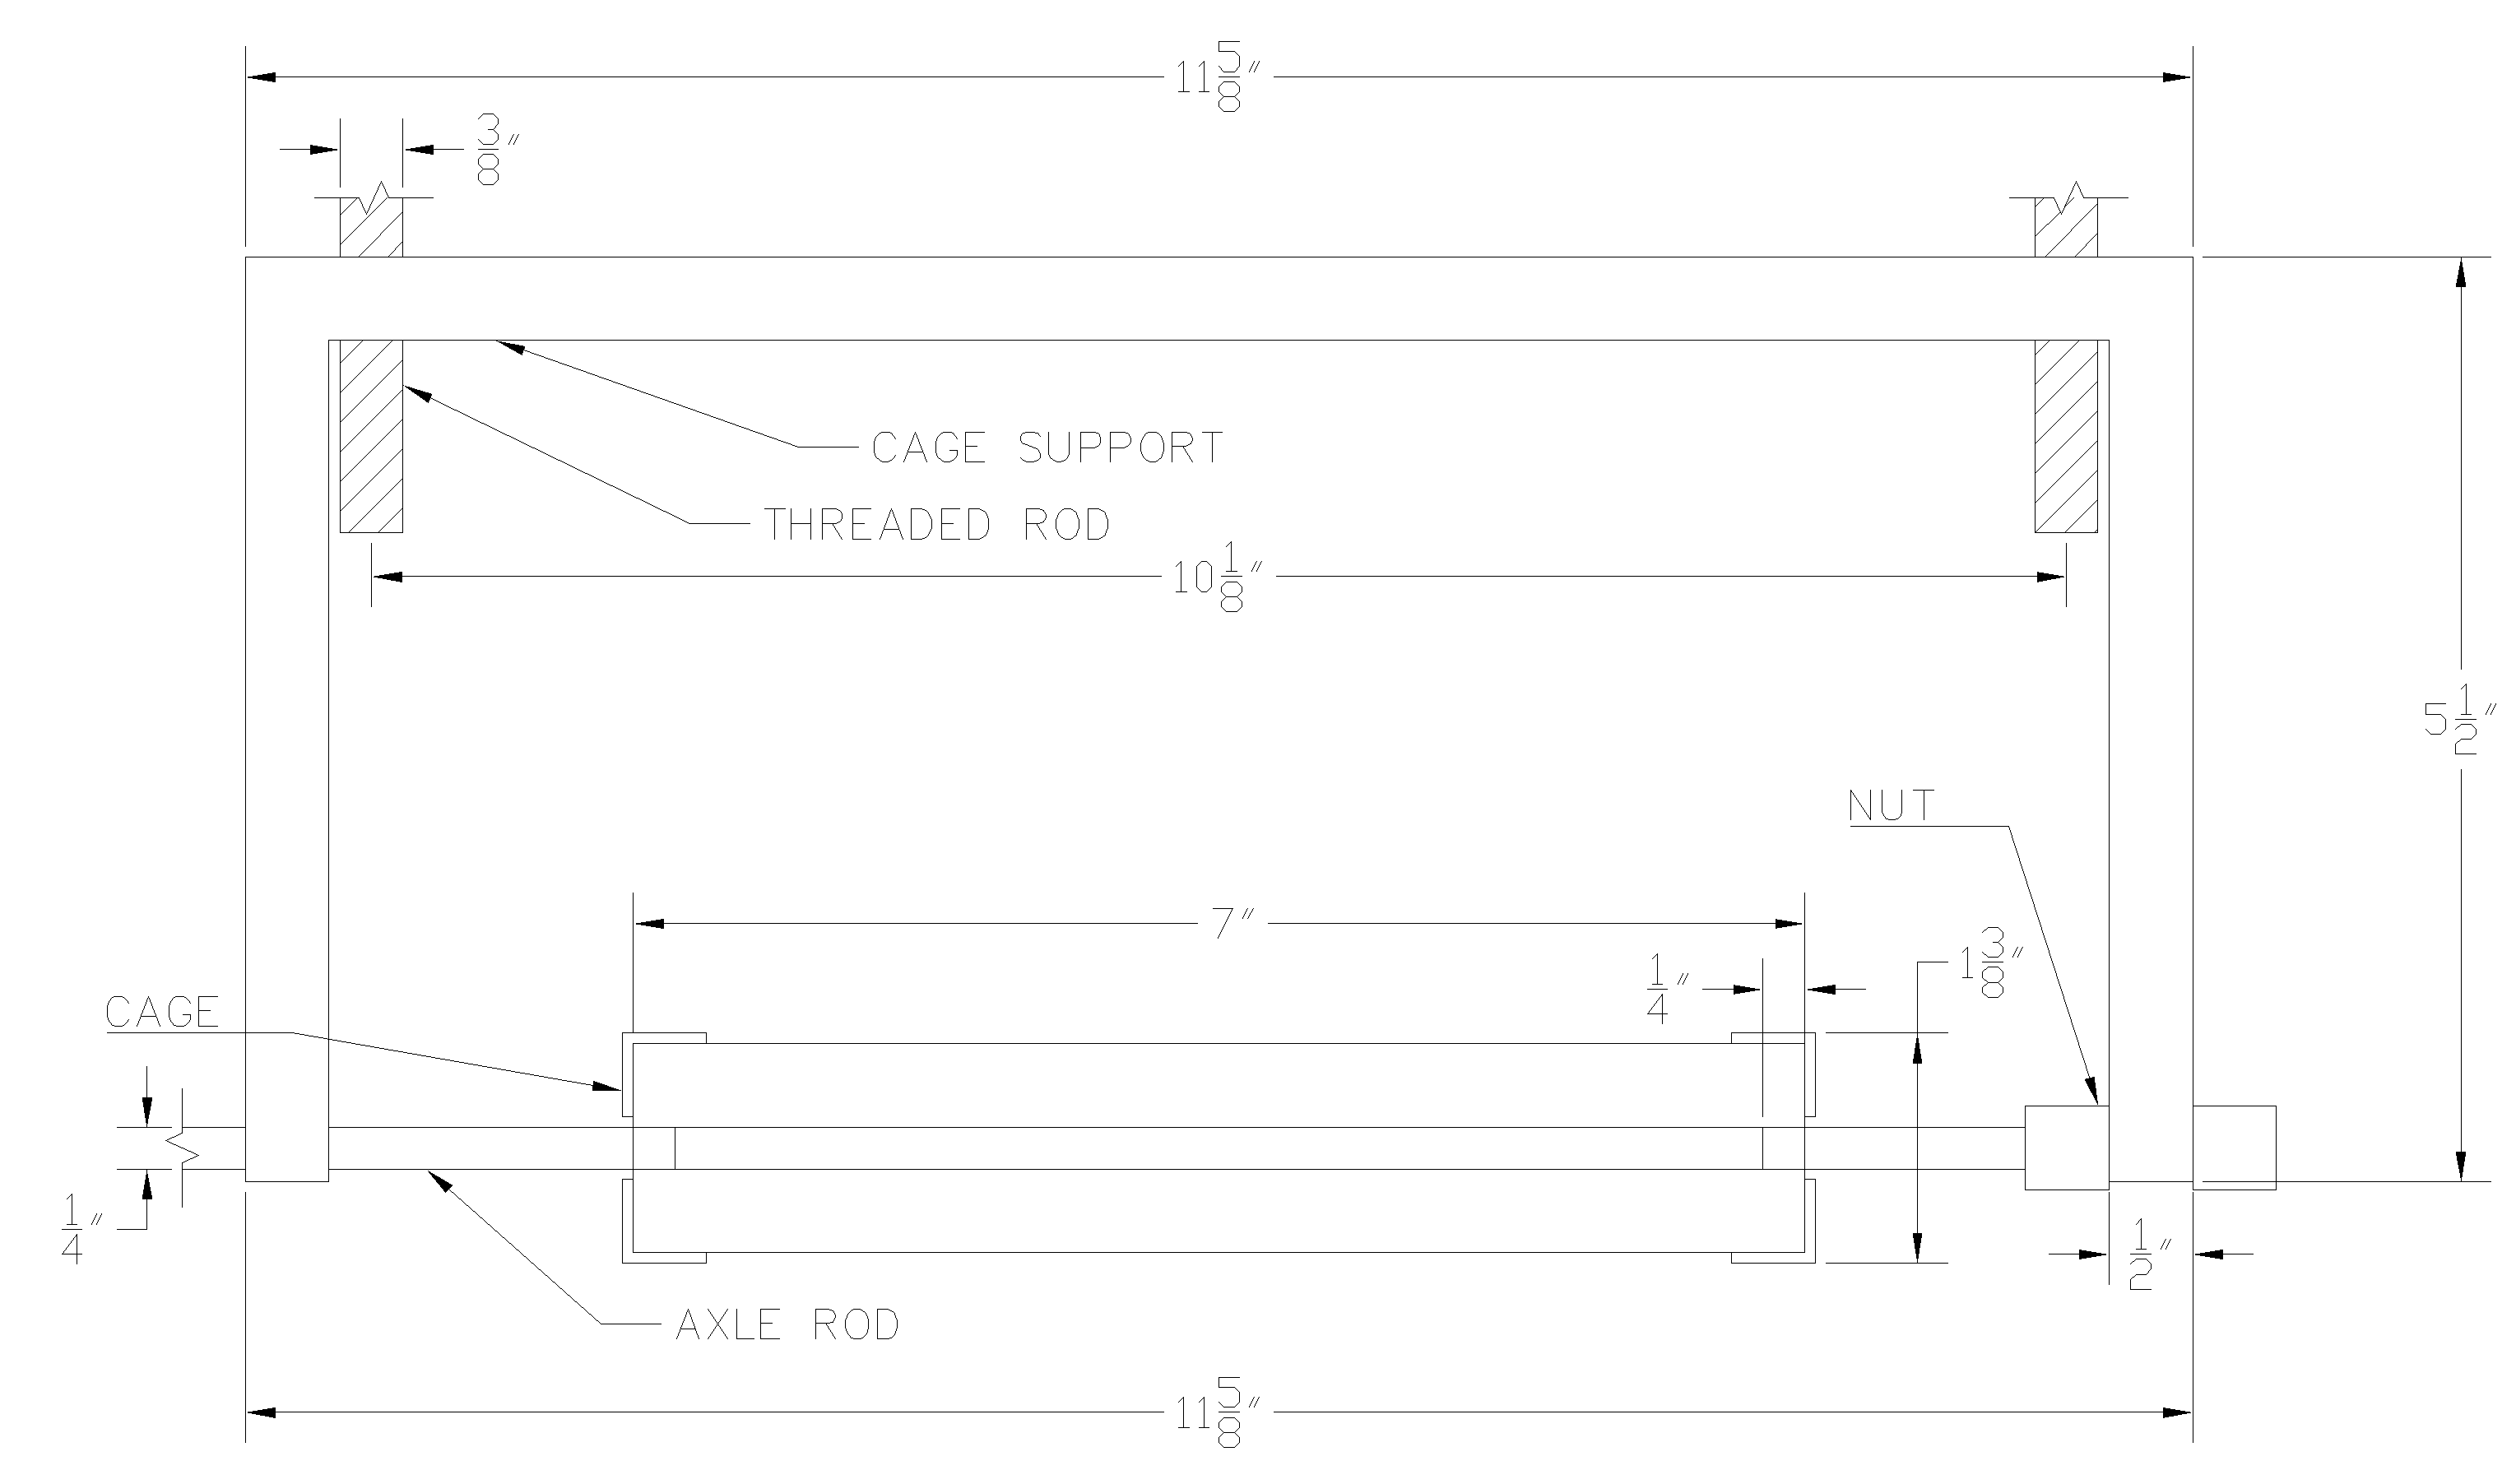
\includegraphics[width=0.6\linewidth]{res/cage.png}
  \caption{The cage design}
  \label{fig:cage}
\end{figure}

The cage-based design features two identical wired baskets, shown in Figure \ref{fig:cage basket}.

\begin{figure}[H]
  \centering
  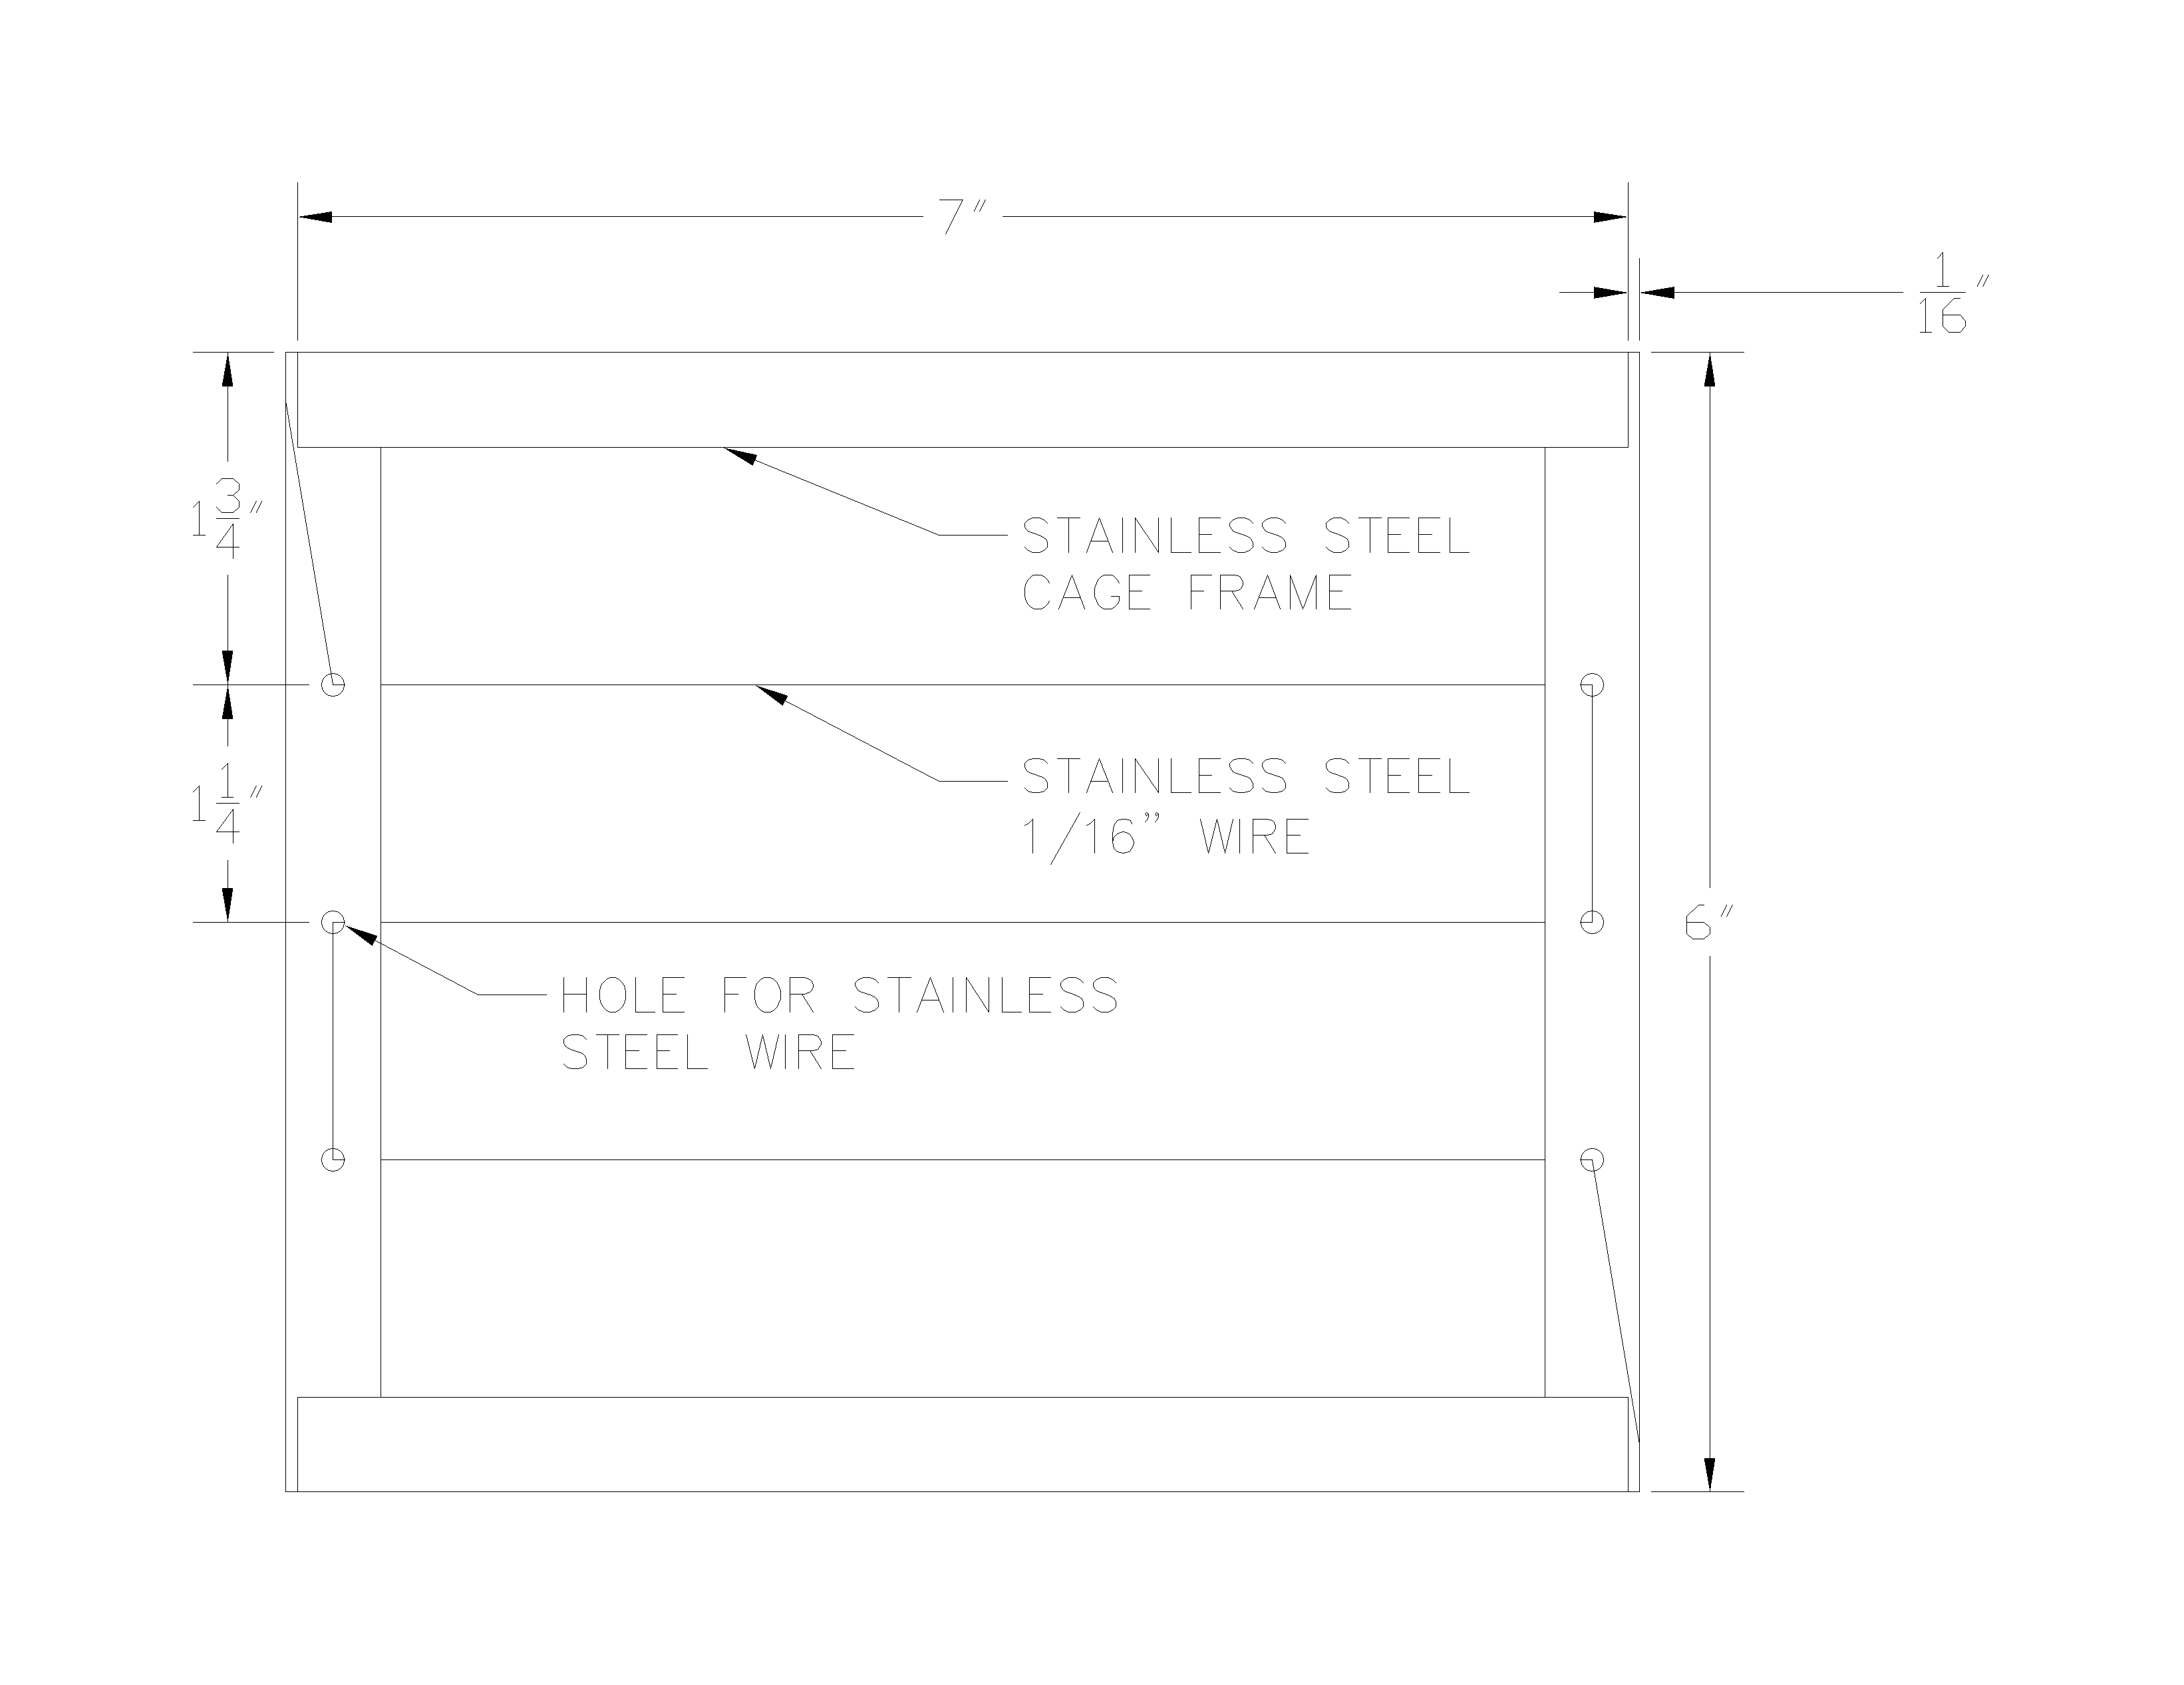
\includegraphics[width=0.6\linewidth]{res/cage_basket.png}
  \caption{The basket from the cage design}
  \label{fig:cage basket}
\end{figure}

Each basket is built from two 6” stainless steel angle bars, and two 7” stainless steel angle bars.
The 7” stainless steel bars rest atop the 6” stainless steel bars, and are connected with angle brackets.
This ordering is important, because the wires run the length of the baskets, not the width.
Placing the shorter bars on the bottom and passing the wires downwards through them guarantees that the wire is the lowest point of the basket, ensuring that the steak is not suspended above the pan.
The wire is wrapped around a corner screw before being passed downwards through the bar and across the length of the basket.
At the other end, the wire is passed upwards through the bar, run along the top of the bar to the next hole, run back downwards through the hole, and across the length of the basket once again.
This pattern repeats at the other end before finally being passed upwards through the last hole and wrapped around the opposite corner screw.

Figure \ref{fig:cage bars} below shows the bars used to construct the baskets.

\begin{figure}[H]
  \centering
  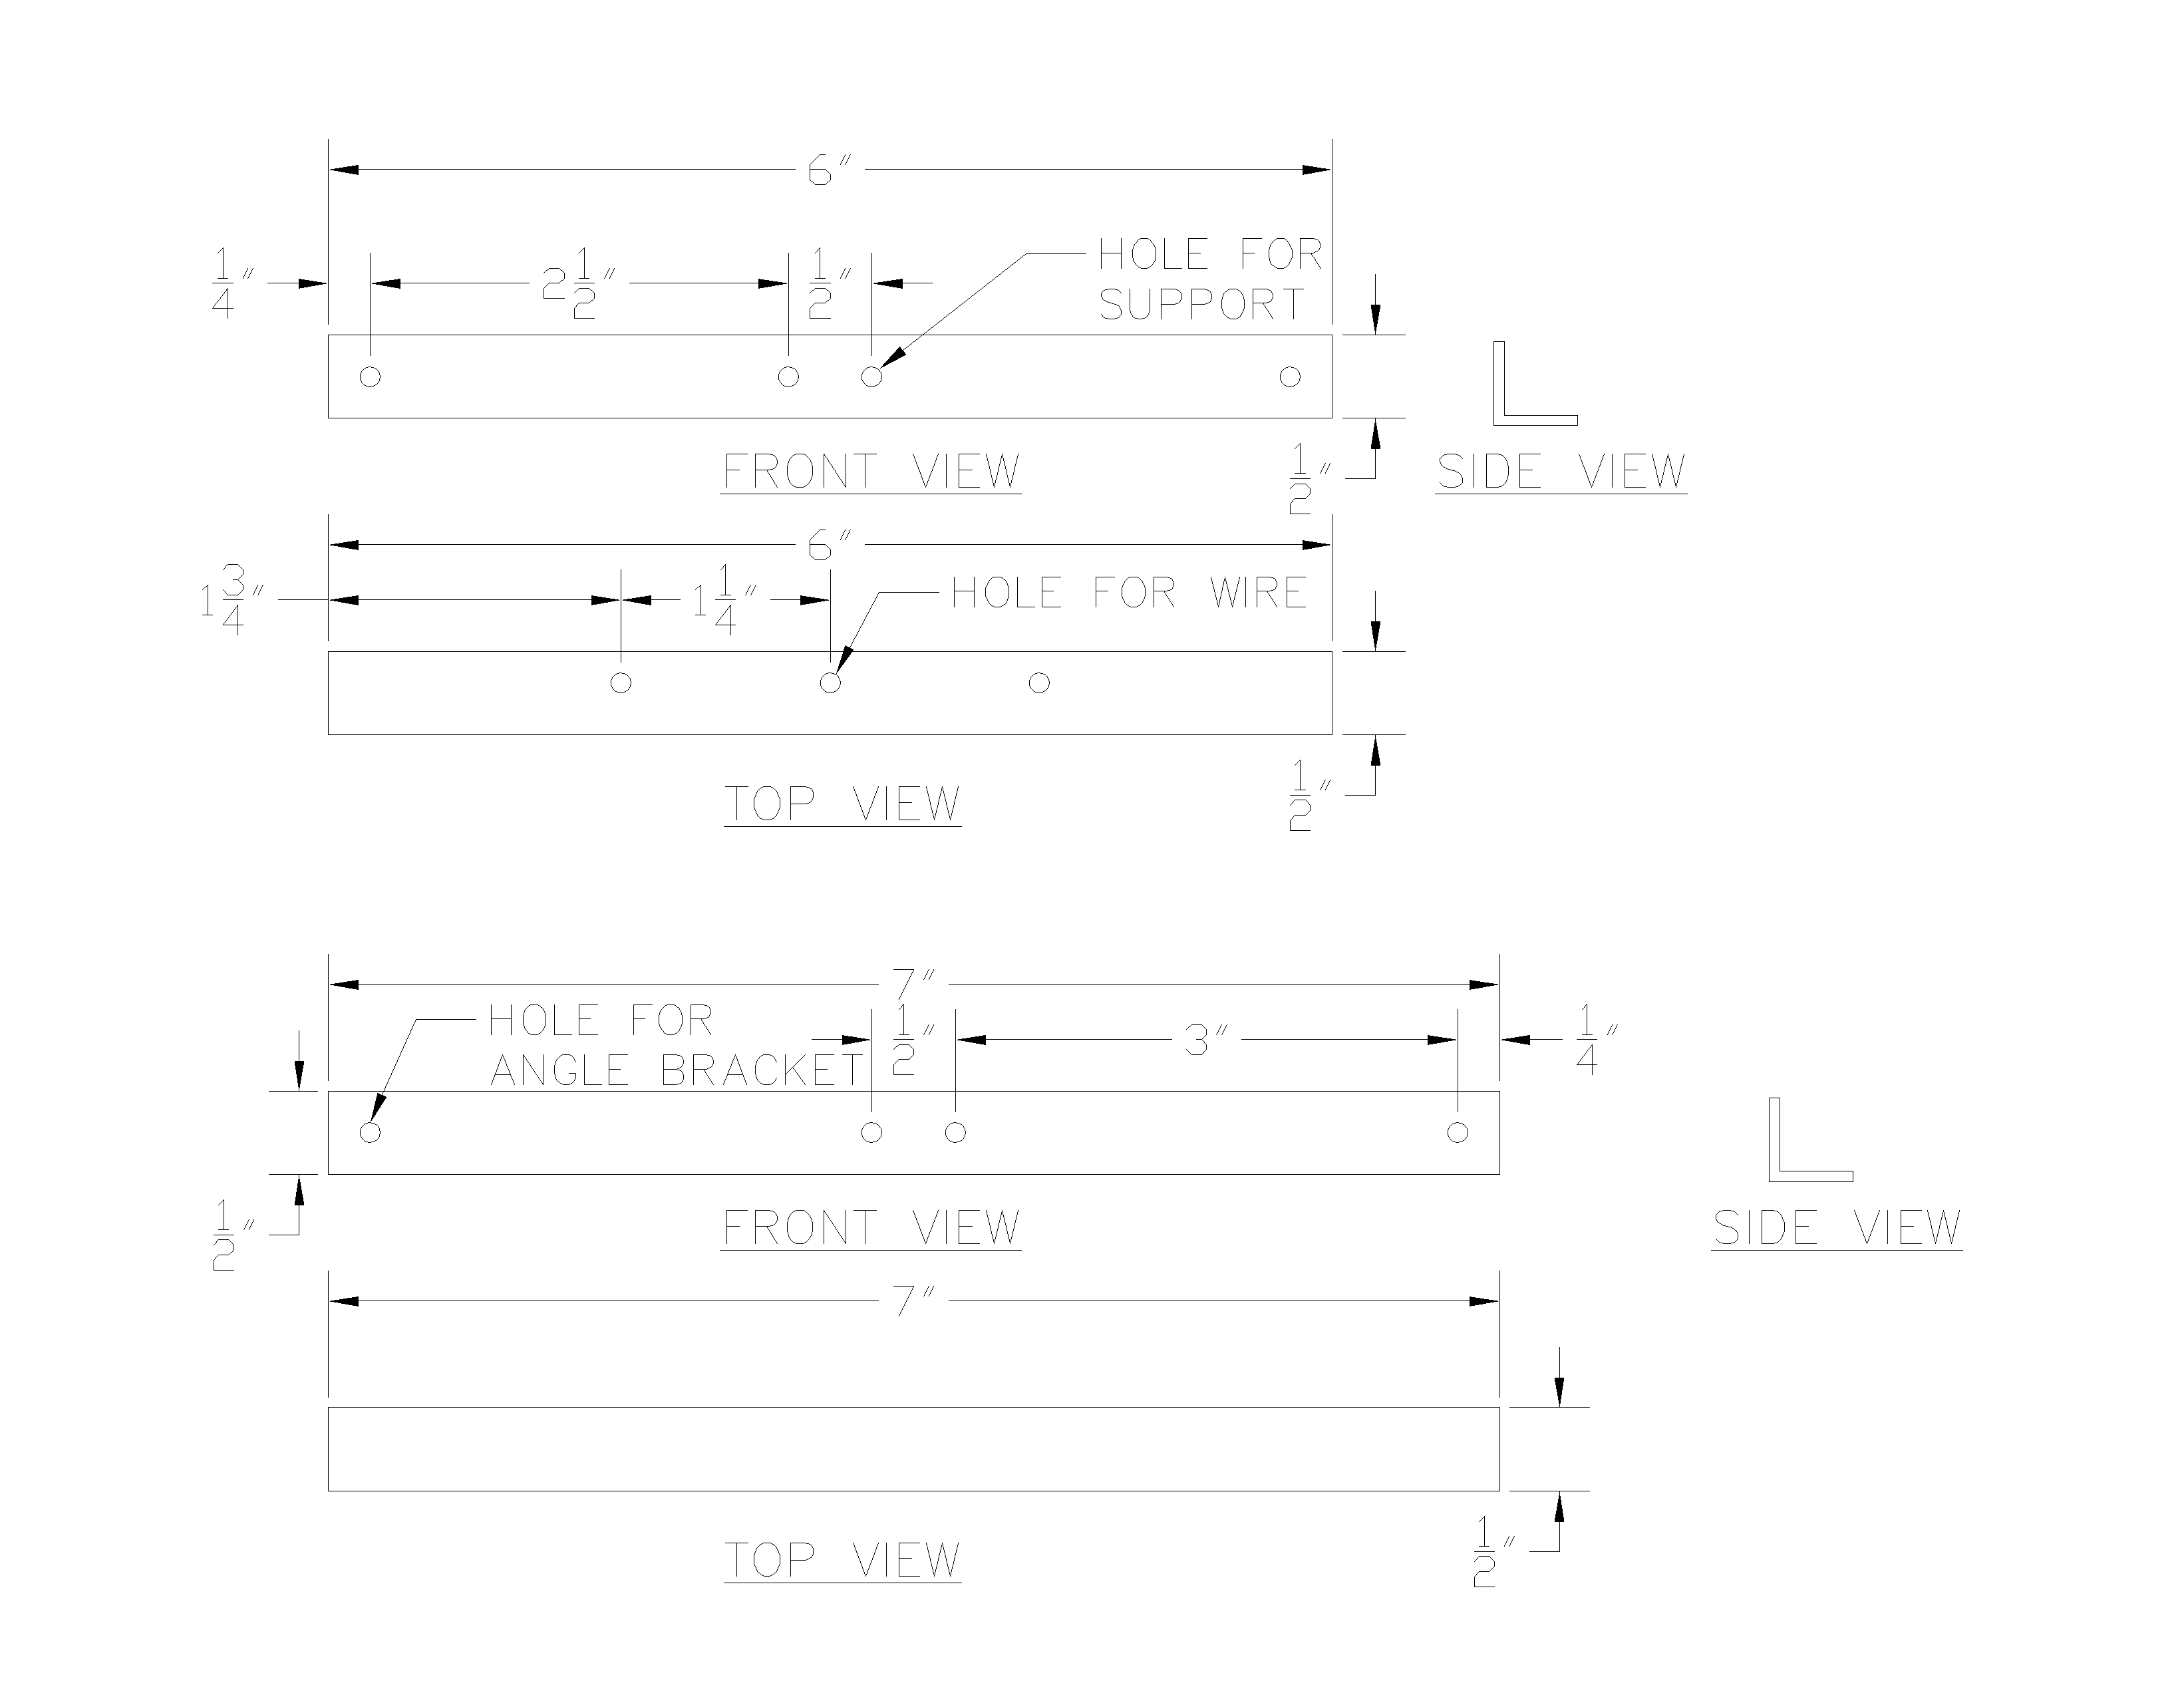
\includegraphics[width=0.6\linewidth]{res/cage_bar.png}
  \caption{The bar from the basket of the cage design}
  \label{fig:cage bars}
\end{figure}

The 6” bars feature three holes on their vertical faces, one at each end which are used to bolt the bars to the angle brackets and one in the middle to bolt it to the coupling.
They feature three more holes spread along the horizontal edge through which the stainless steel wire is passed.
The 7” bars are similar to the 6” bars, but feature only the two holes used to bolt them to the angle brackets.

Figure \ref{fig:cage coupling} shows the coupling piece that is used to attach the baskets to the rotational axle.

\begin{figure}[H]
  \centering
  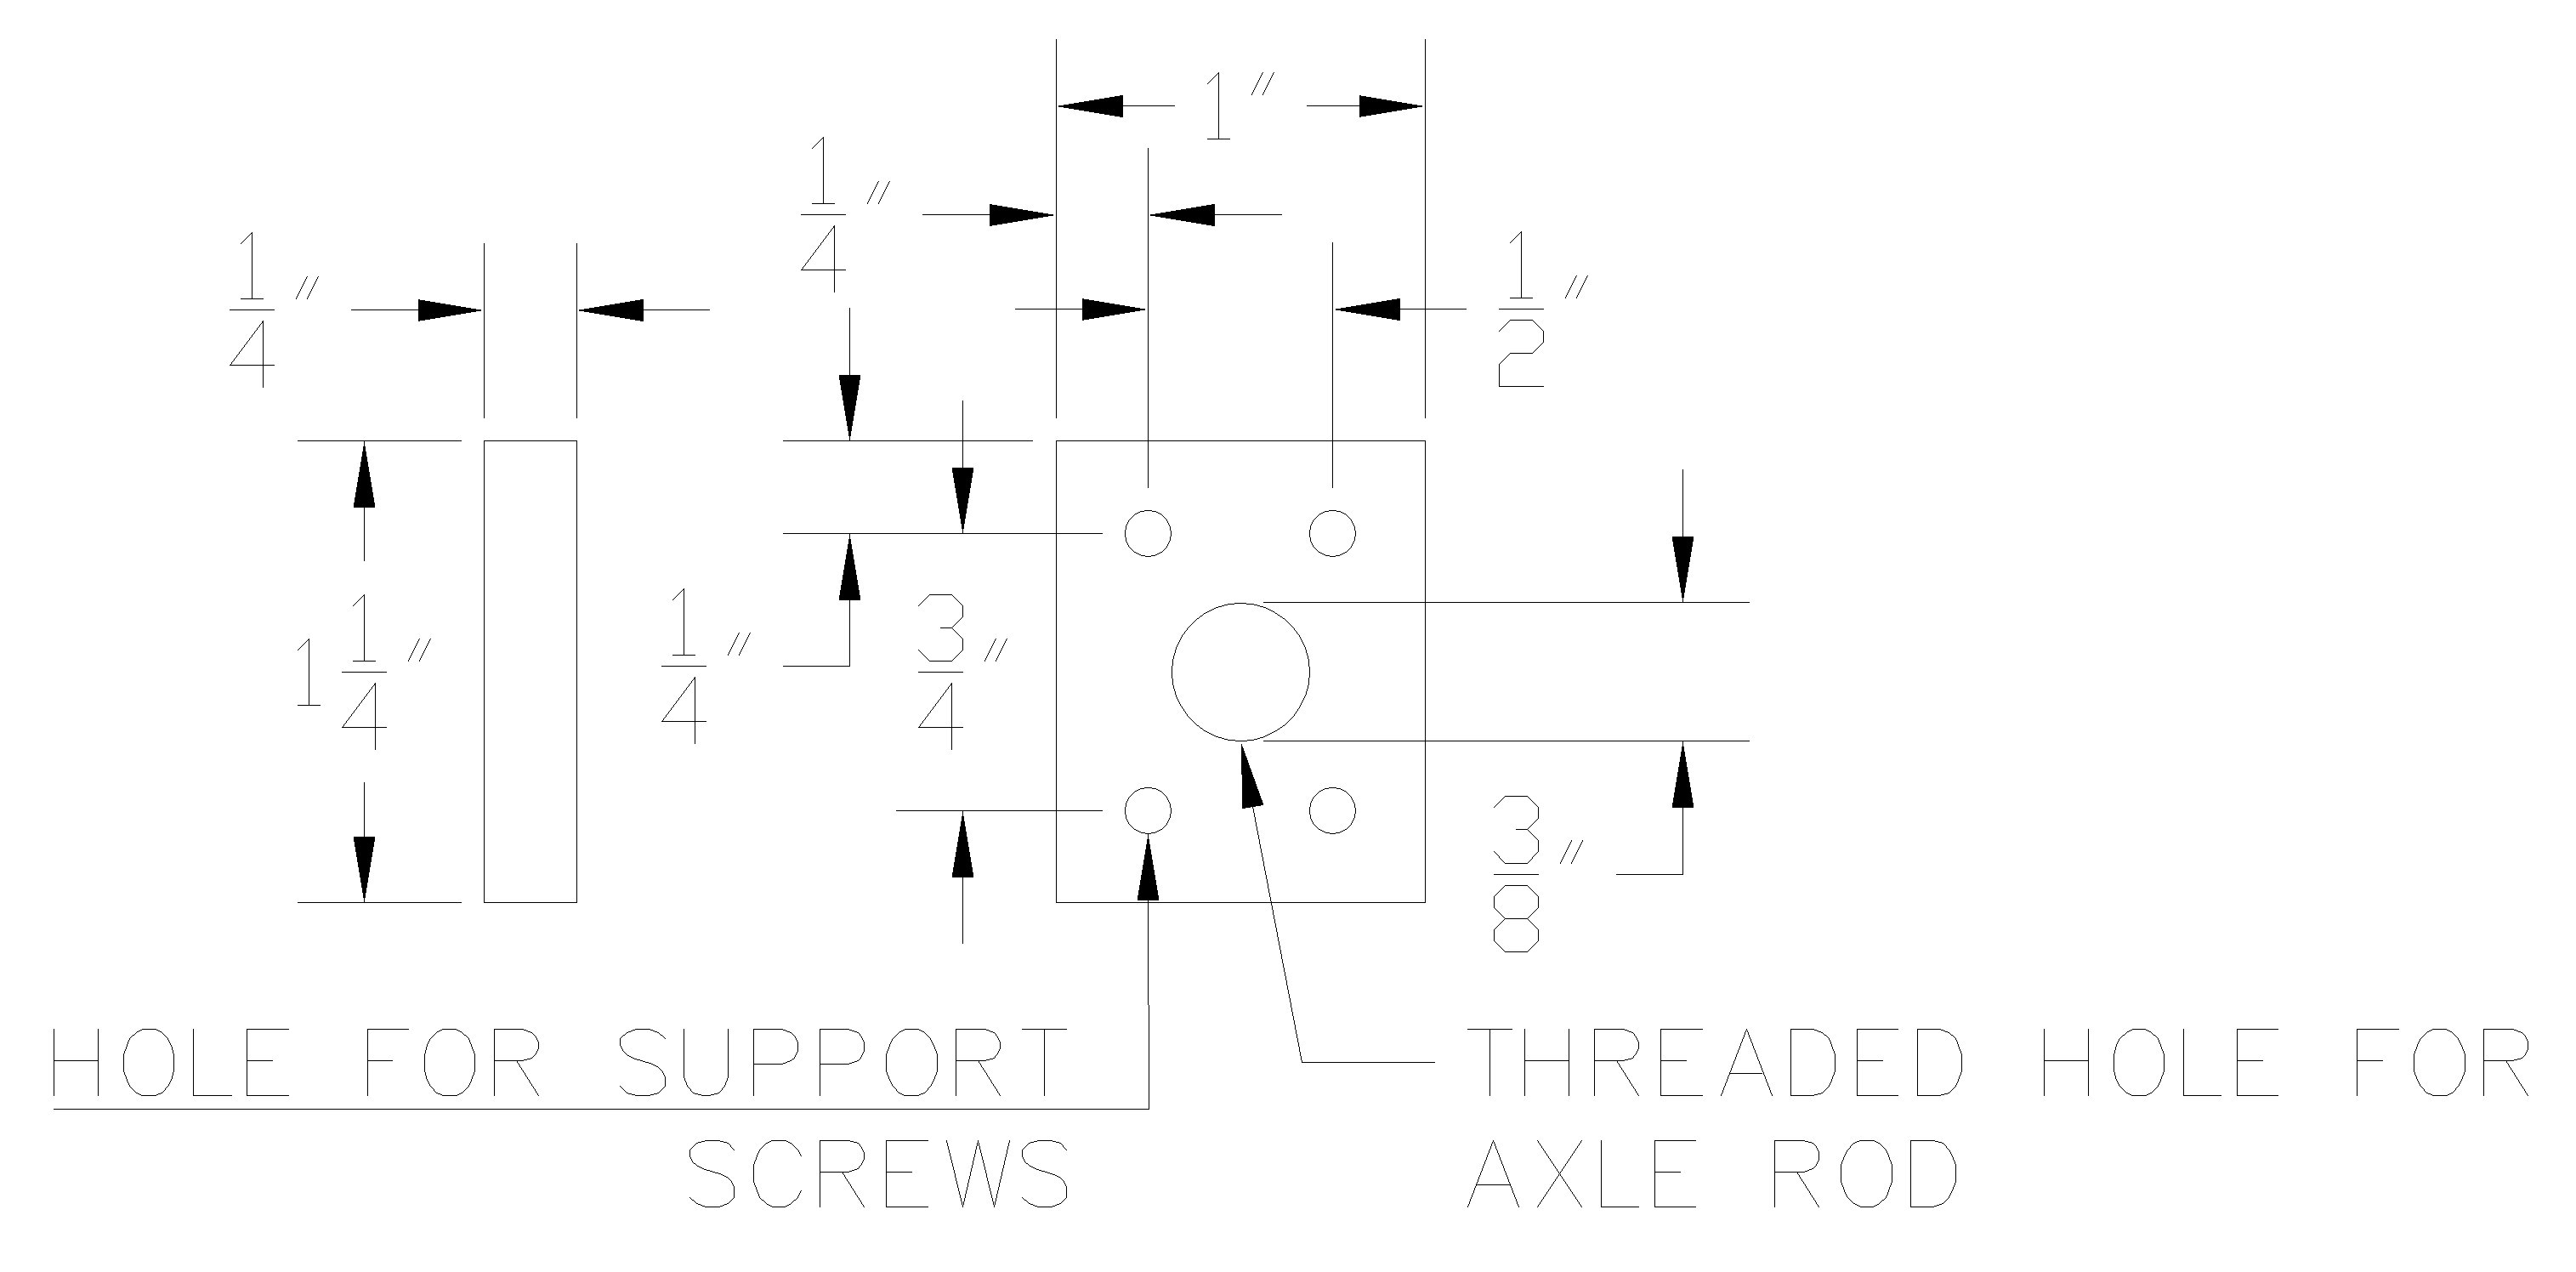
\includegraphics[width=0.6\linewidth]{res/cage_coupling.png}
  \caption{The coupling from the basket of the cage design}
  \label{fig:cage coupling}
\end{figure}

The coupling is a simple block of stainless steel with three tapped holes drilled into one of its faces.
The upper and lower holes are used to bolt the coupling to the upper and lower baskets, and the middle hole is used to attach the baskets to the axle that is used to rotate the apparatus.

Figure \ref{fig:cage ball screw adapter} shows the coupler that is used to connect the cage to the ball screws.

\begin{figure}[H]
  \centering
  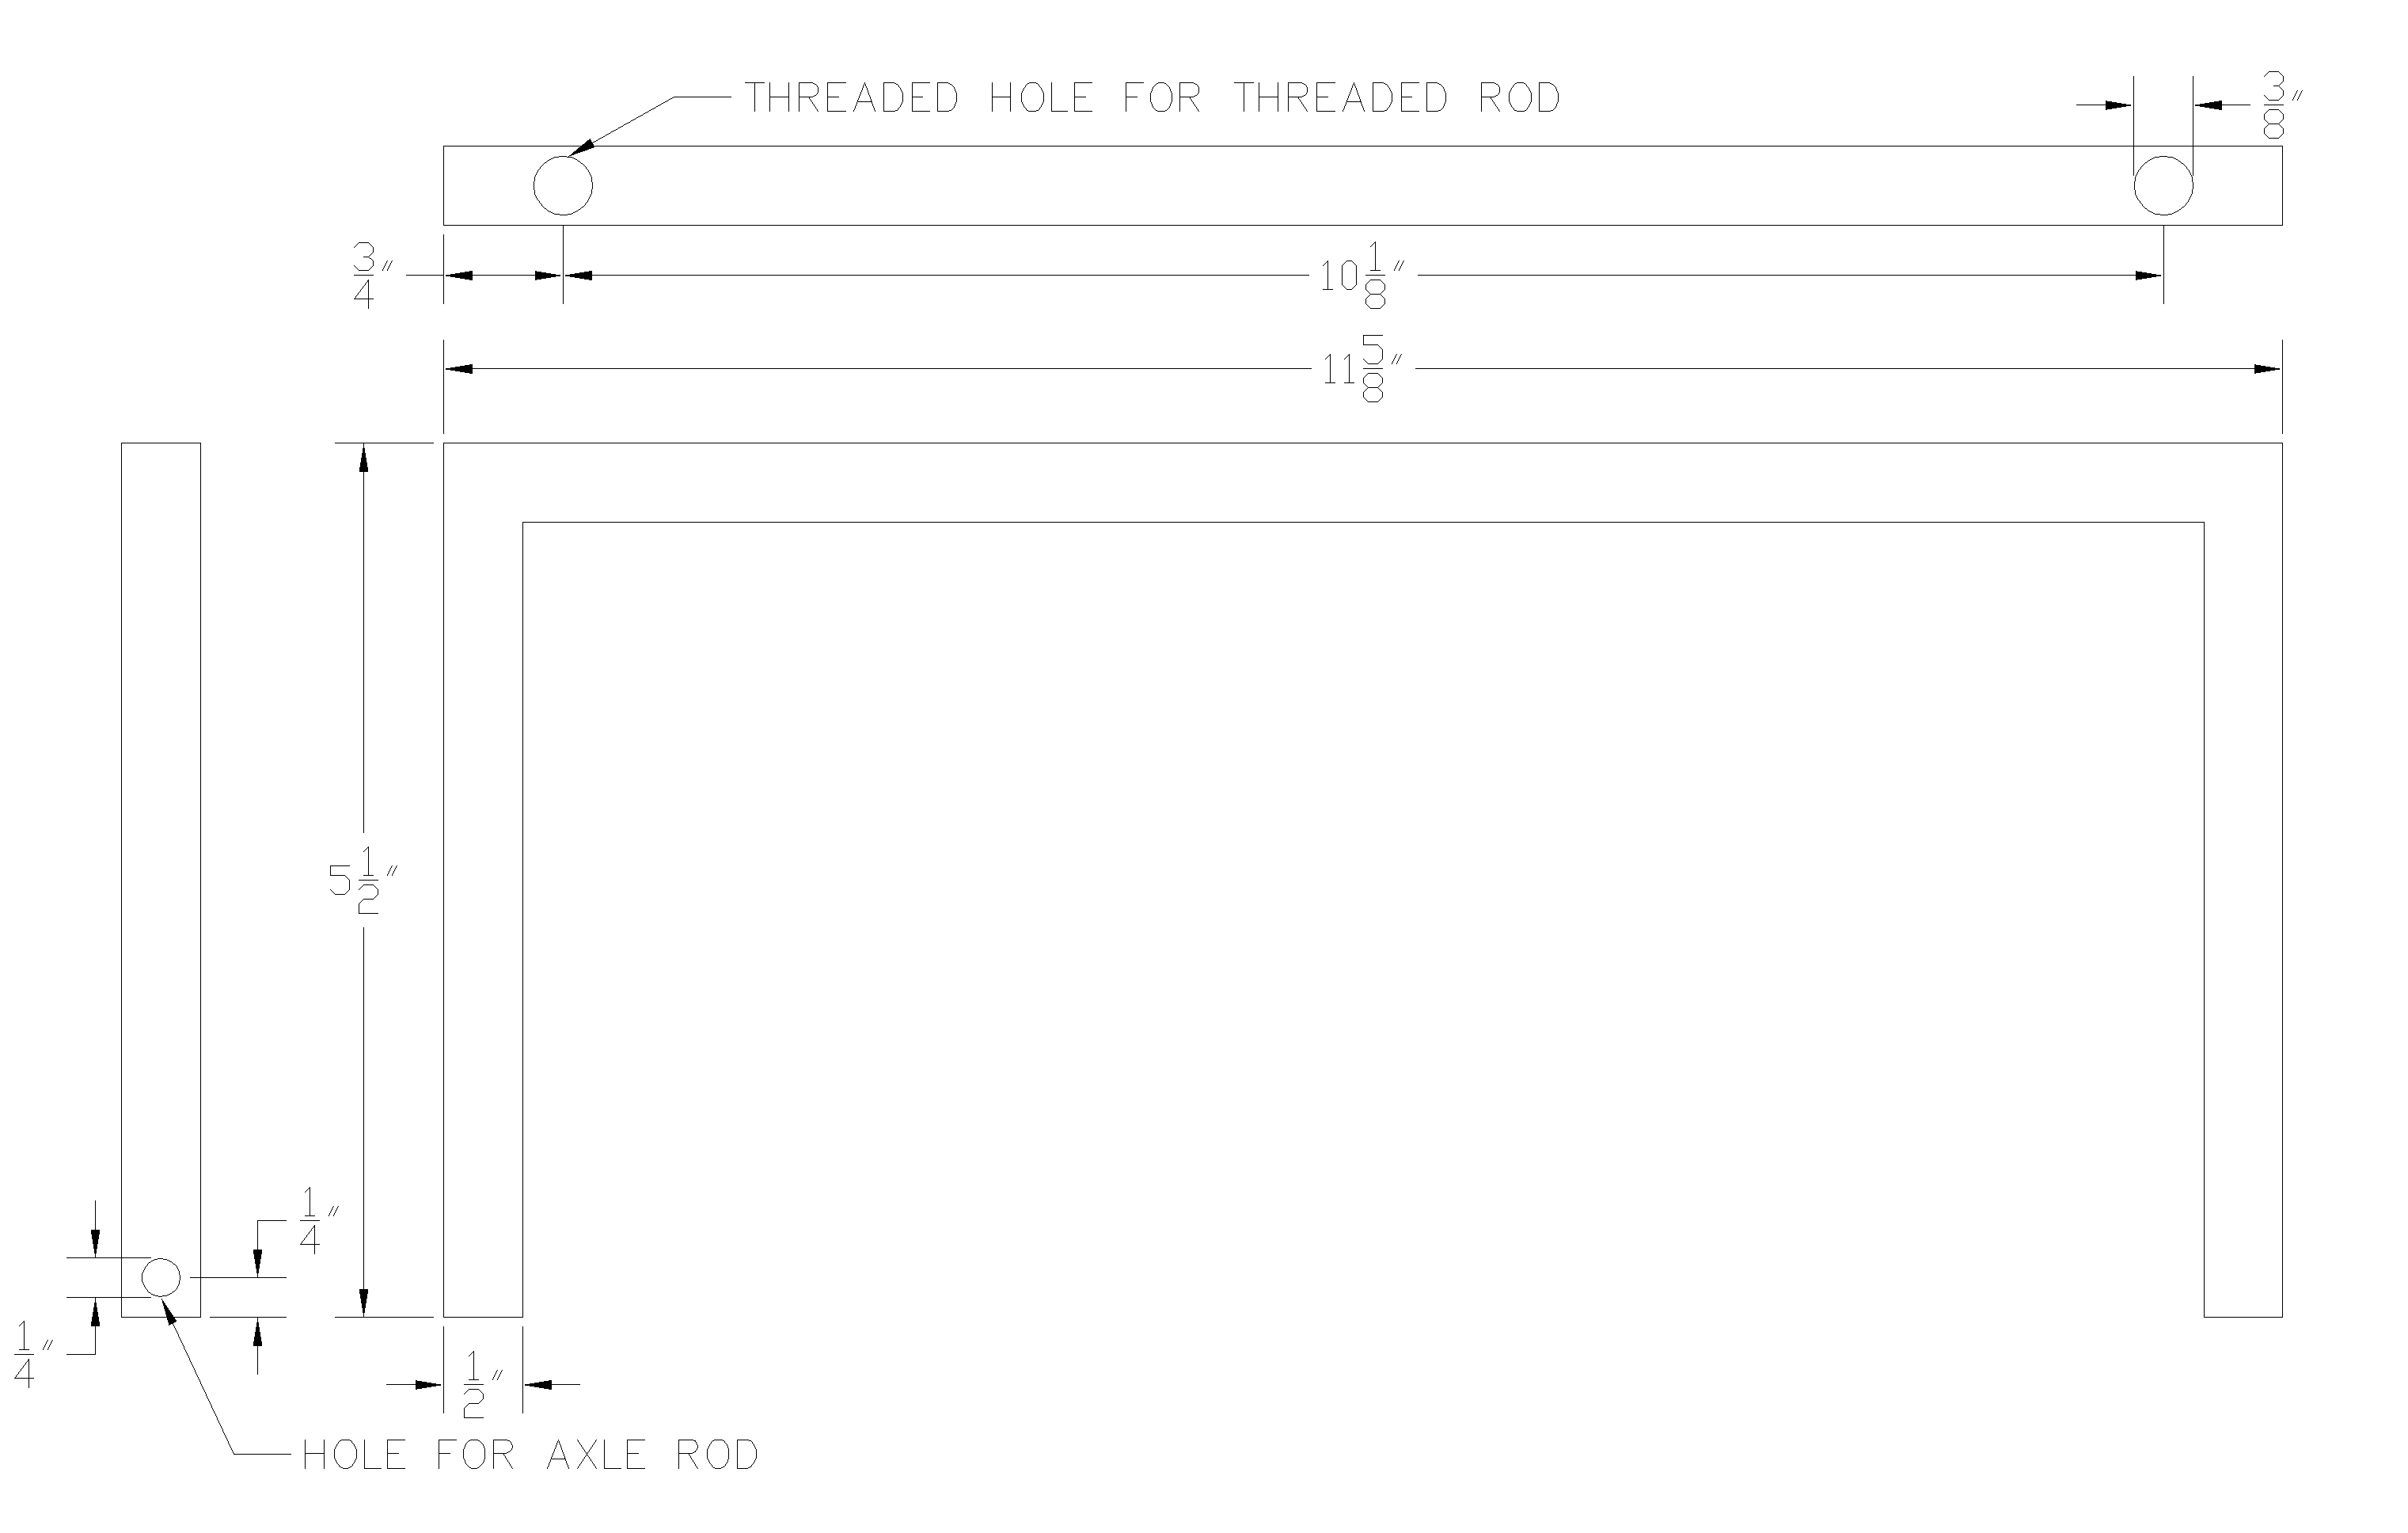
\includegraphics[width=0.6\linewidth]{res/cage_ball_screw_adapter.png}
  \caption{The ball screw adapter from the cage design}
  \label{fig:cage ball screw adapter}
\end{figure}

The coupler is a long piece of metal with two holes into which the ball screws fit, and is bent into a u shape.
The arms of the u hang down towards the cage, and at the end of each is drilled with a hole into which the axle is passed.

Figure \ref{fig:cage axle} shows the rotational axle.

\begin{figure}[H]
  \centering
  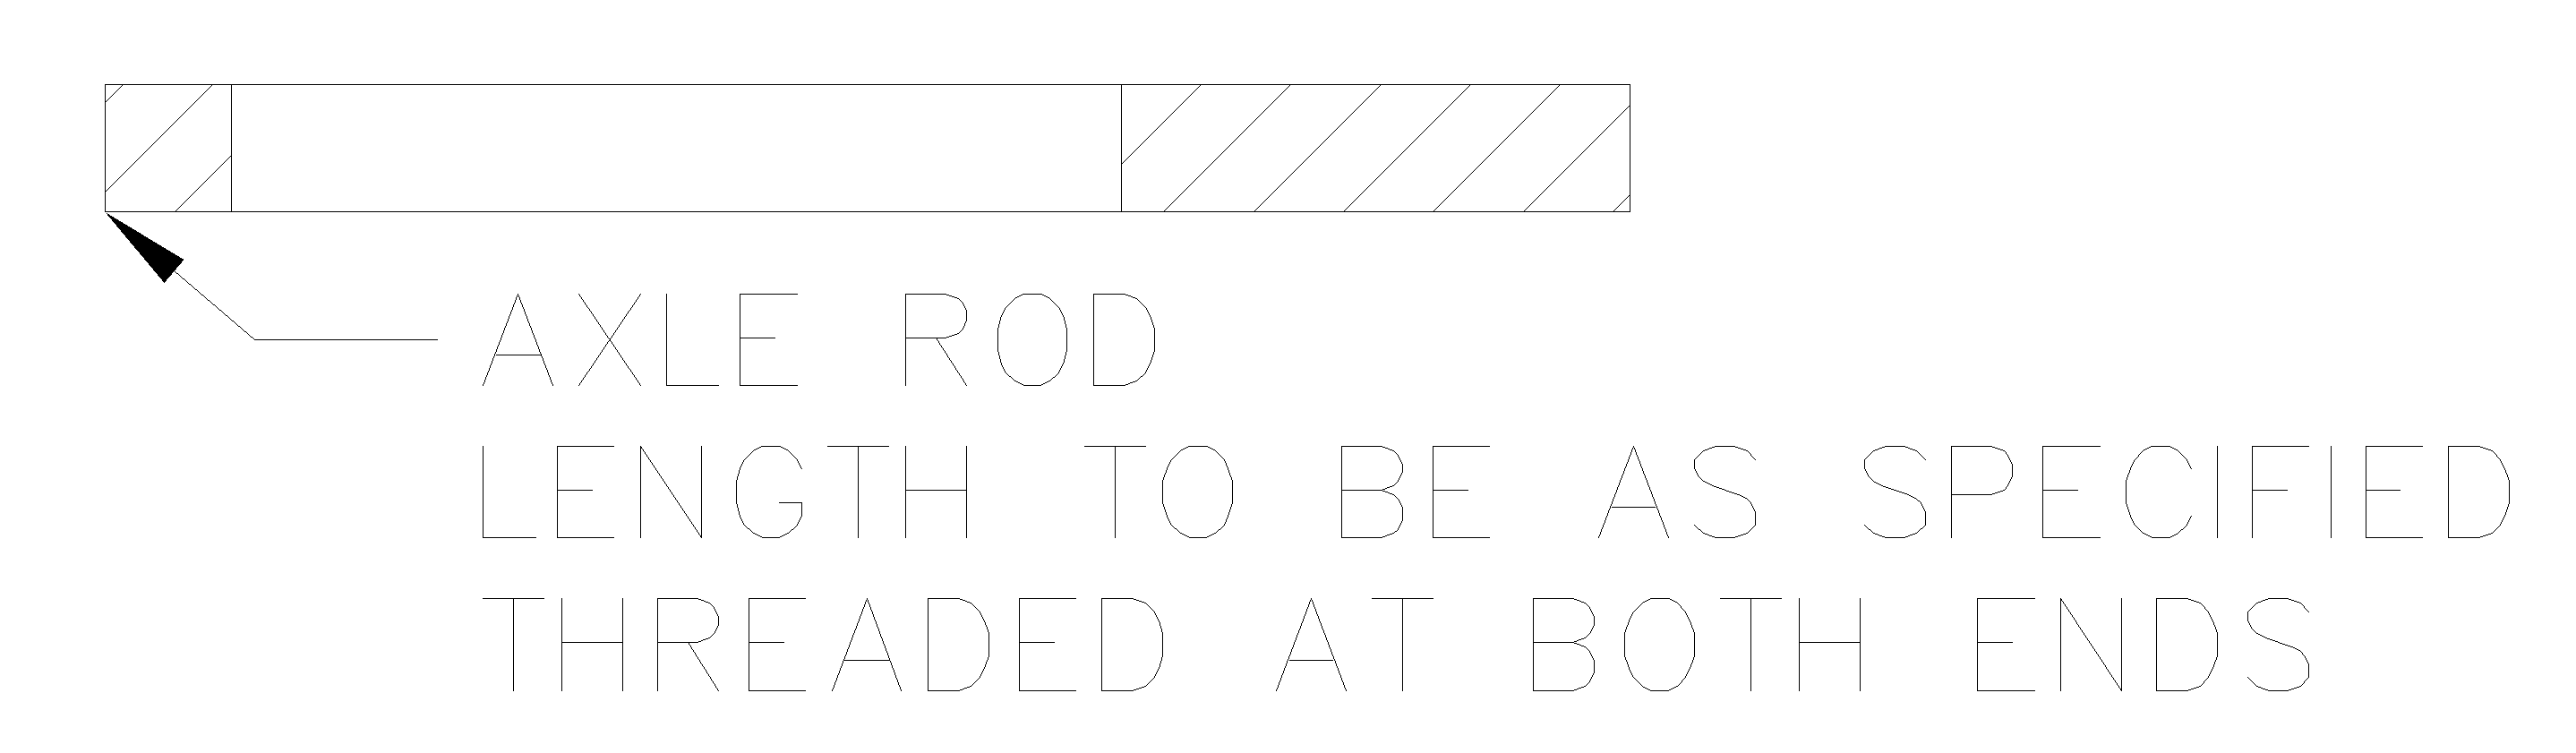
\includegraphics[width=0.4\linewidth]{res/cage_axle.png}
  \caption{The axle from the cage design}
  \label{fig:cage axle}
\end{figure}

The axle is divided into two pieces, each end of which is threaded.
One end of each axle is screwed into the basket coupling and the other end of one is attached to the rotation mechanism, and the other end is simply bolted so the axle is secured between the vertical bars.

The mesh-based design is nearly identical to the cage-based design.
The difference is that a mesh is used in place of the wires.
A diagram of the mesh is shown in Figure \ref{fig:mesh}.

\begin{figure}[H]
  \centering
  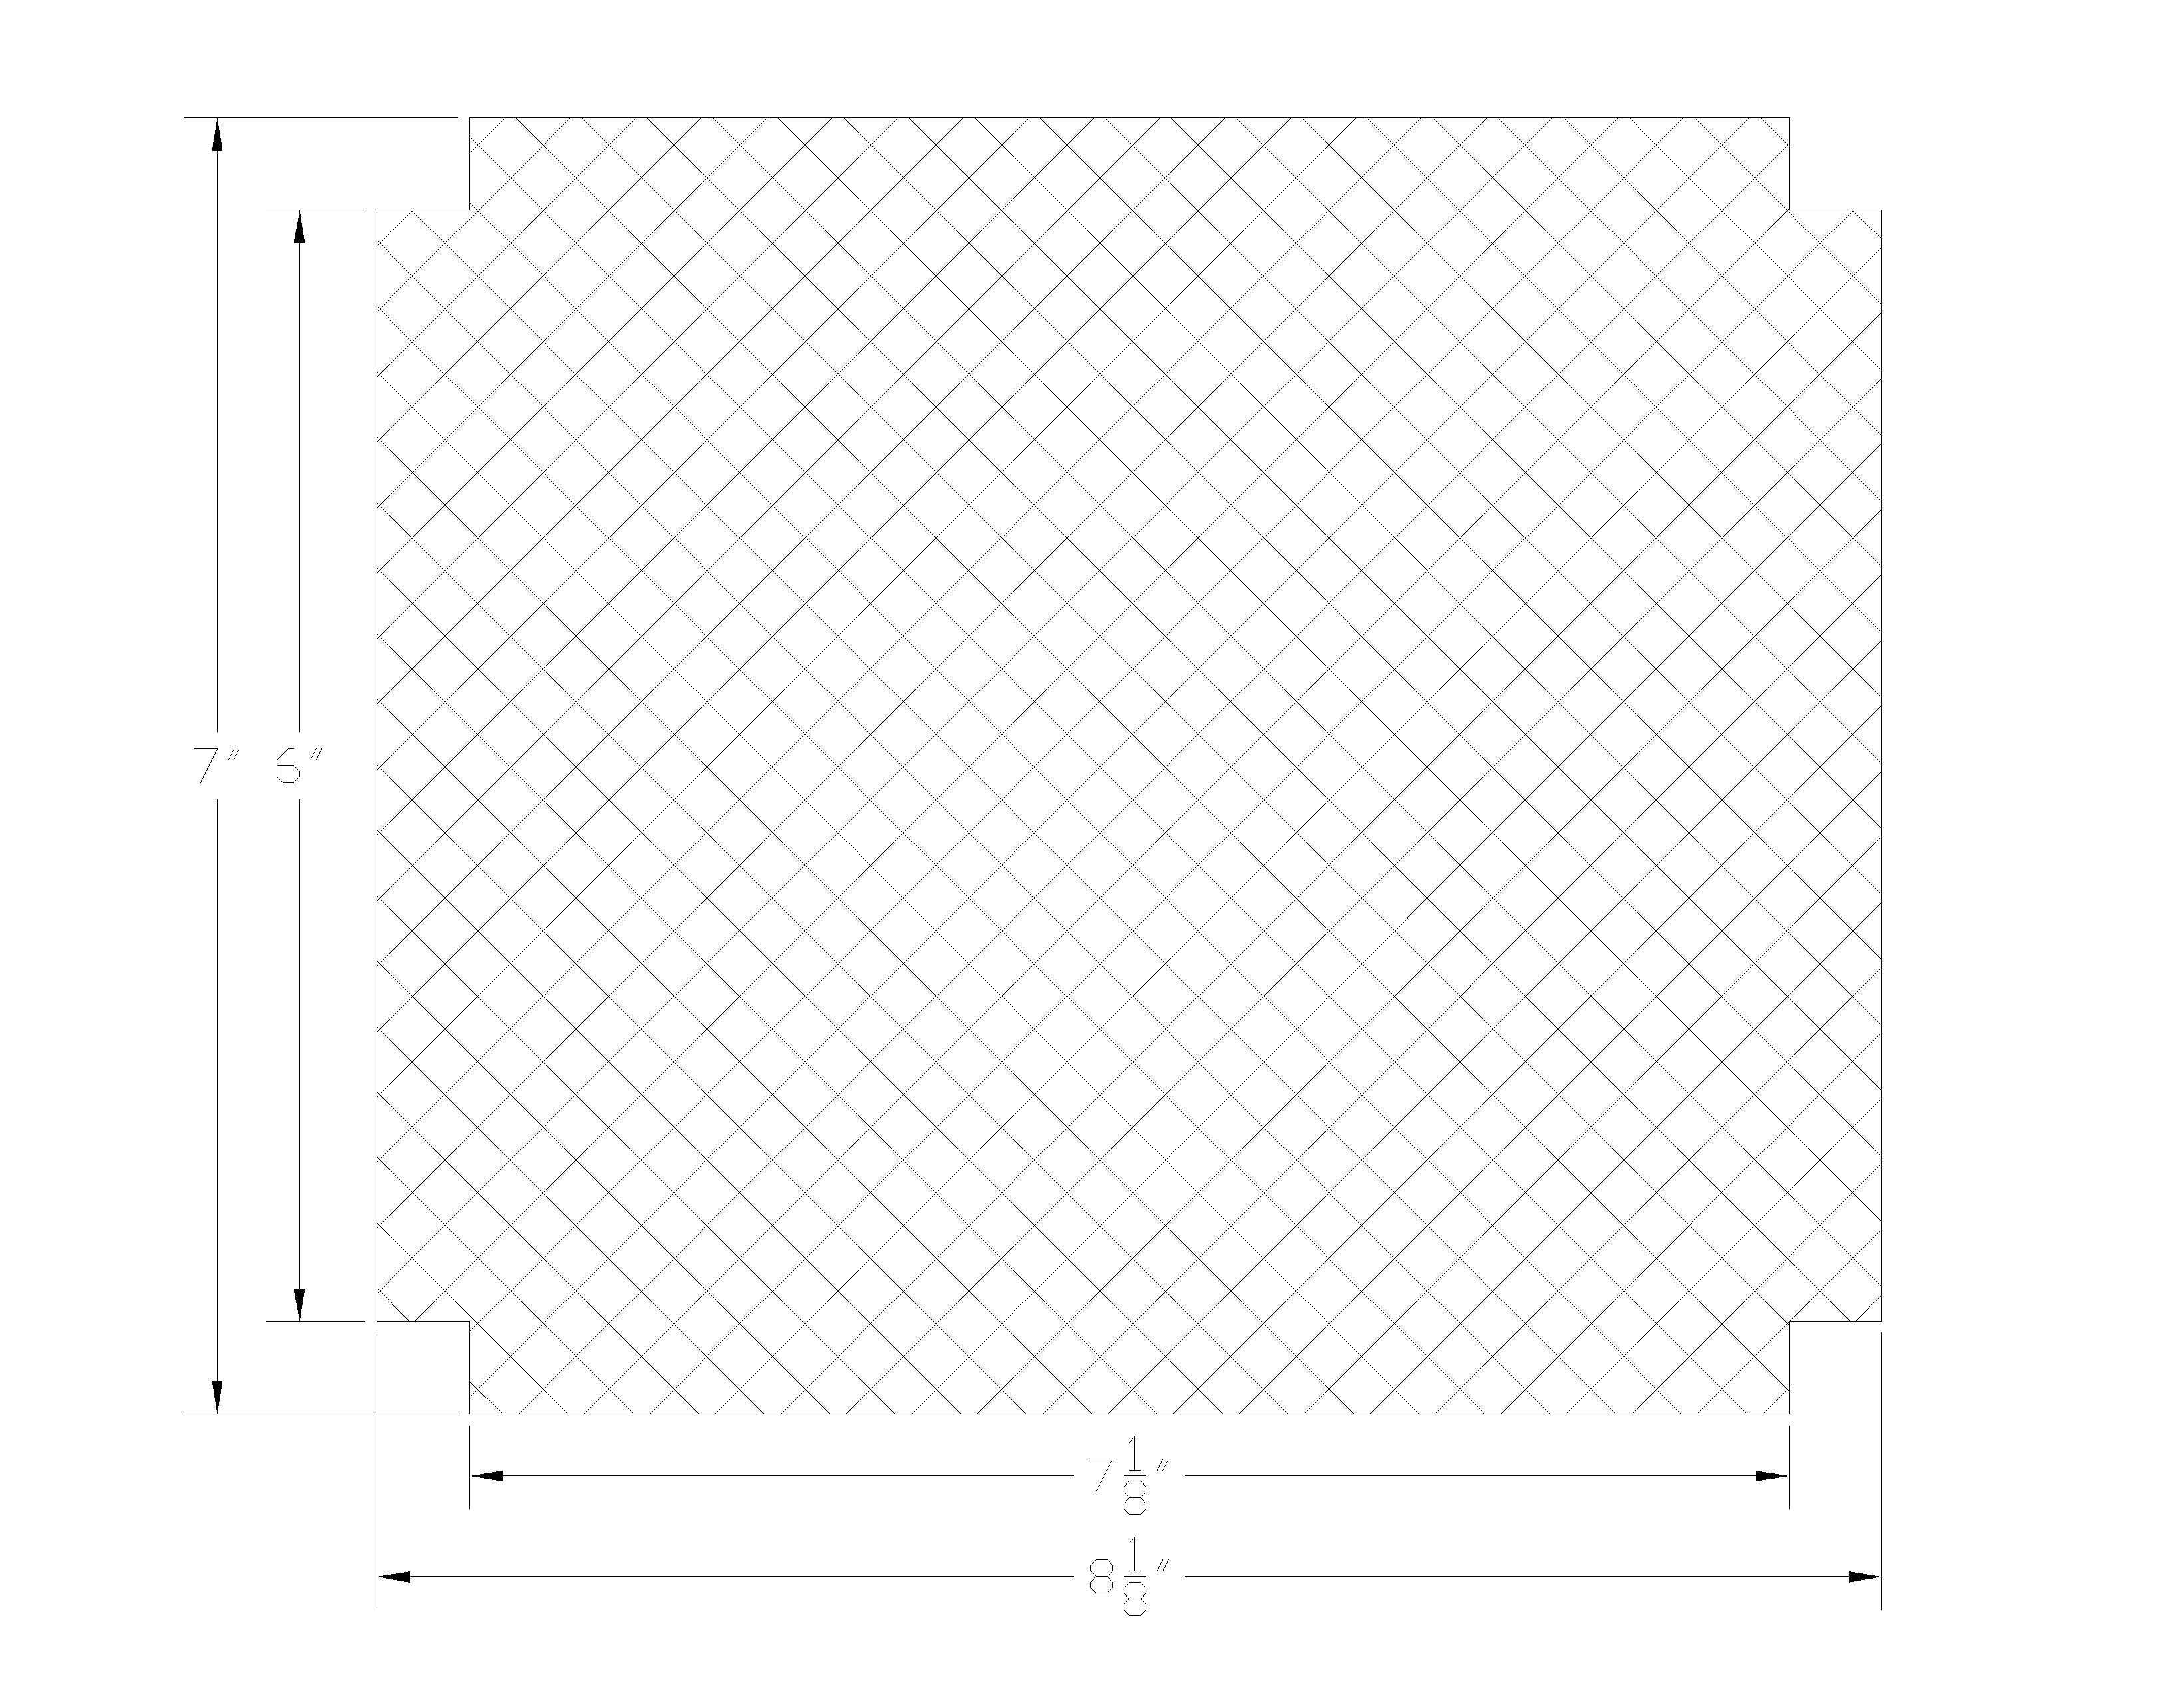
\includegraphics[width=0.6\linewidth]{res/mesh.png}
  \caption{The mesh from the mesh design}
  \label{fig:mesh}
\end{figure}

The mesh is cut at the corners to be wrapped around the edges of the basket, and holes are drilled into it such that the screws that go into the couplings and the angle brackets also secure the mesh to the baskets.

The spatula-based design is significantly different.
The design is displayed in Figure \ref{fig:spatula} below.

\begin{figure}[H]
  \centering
  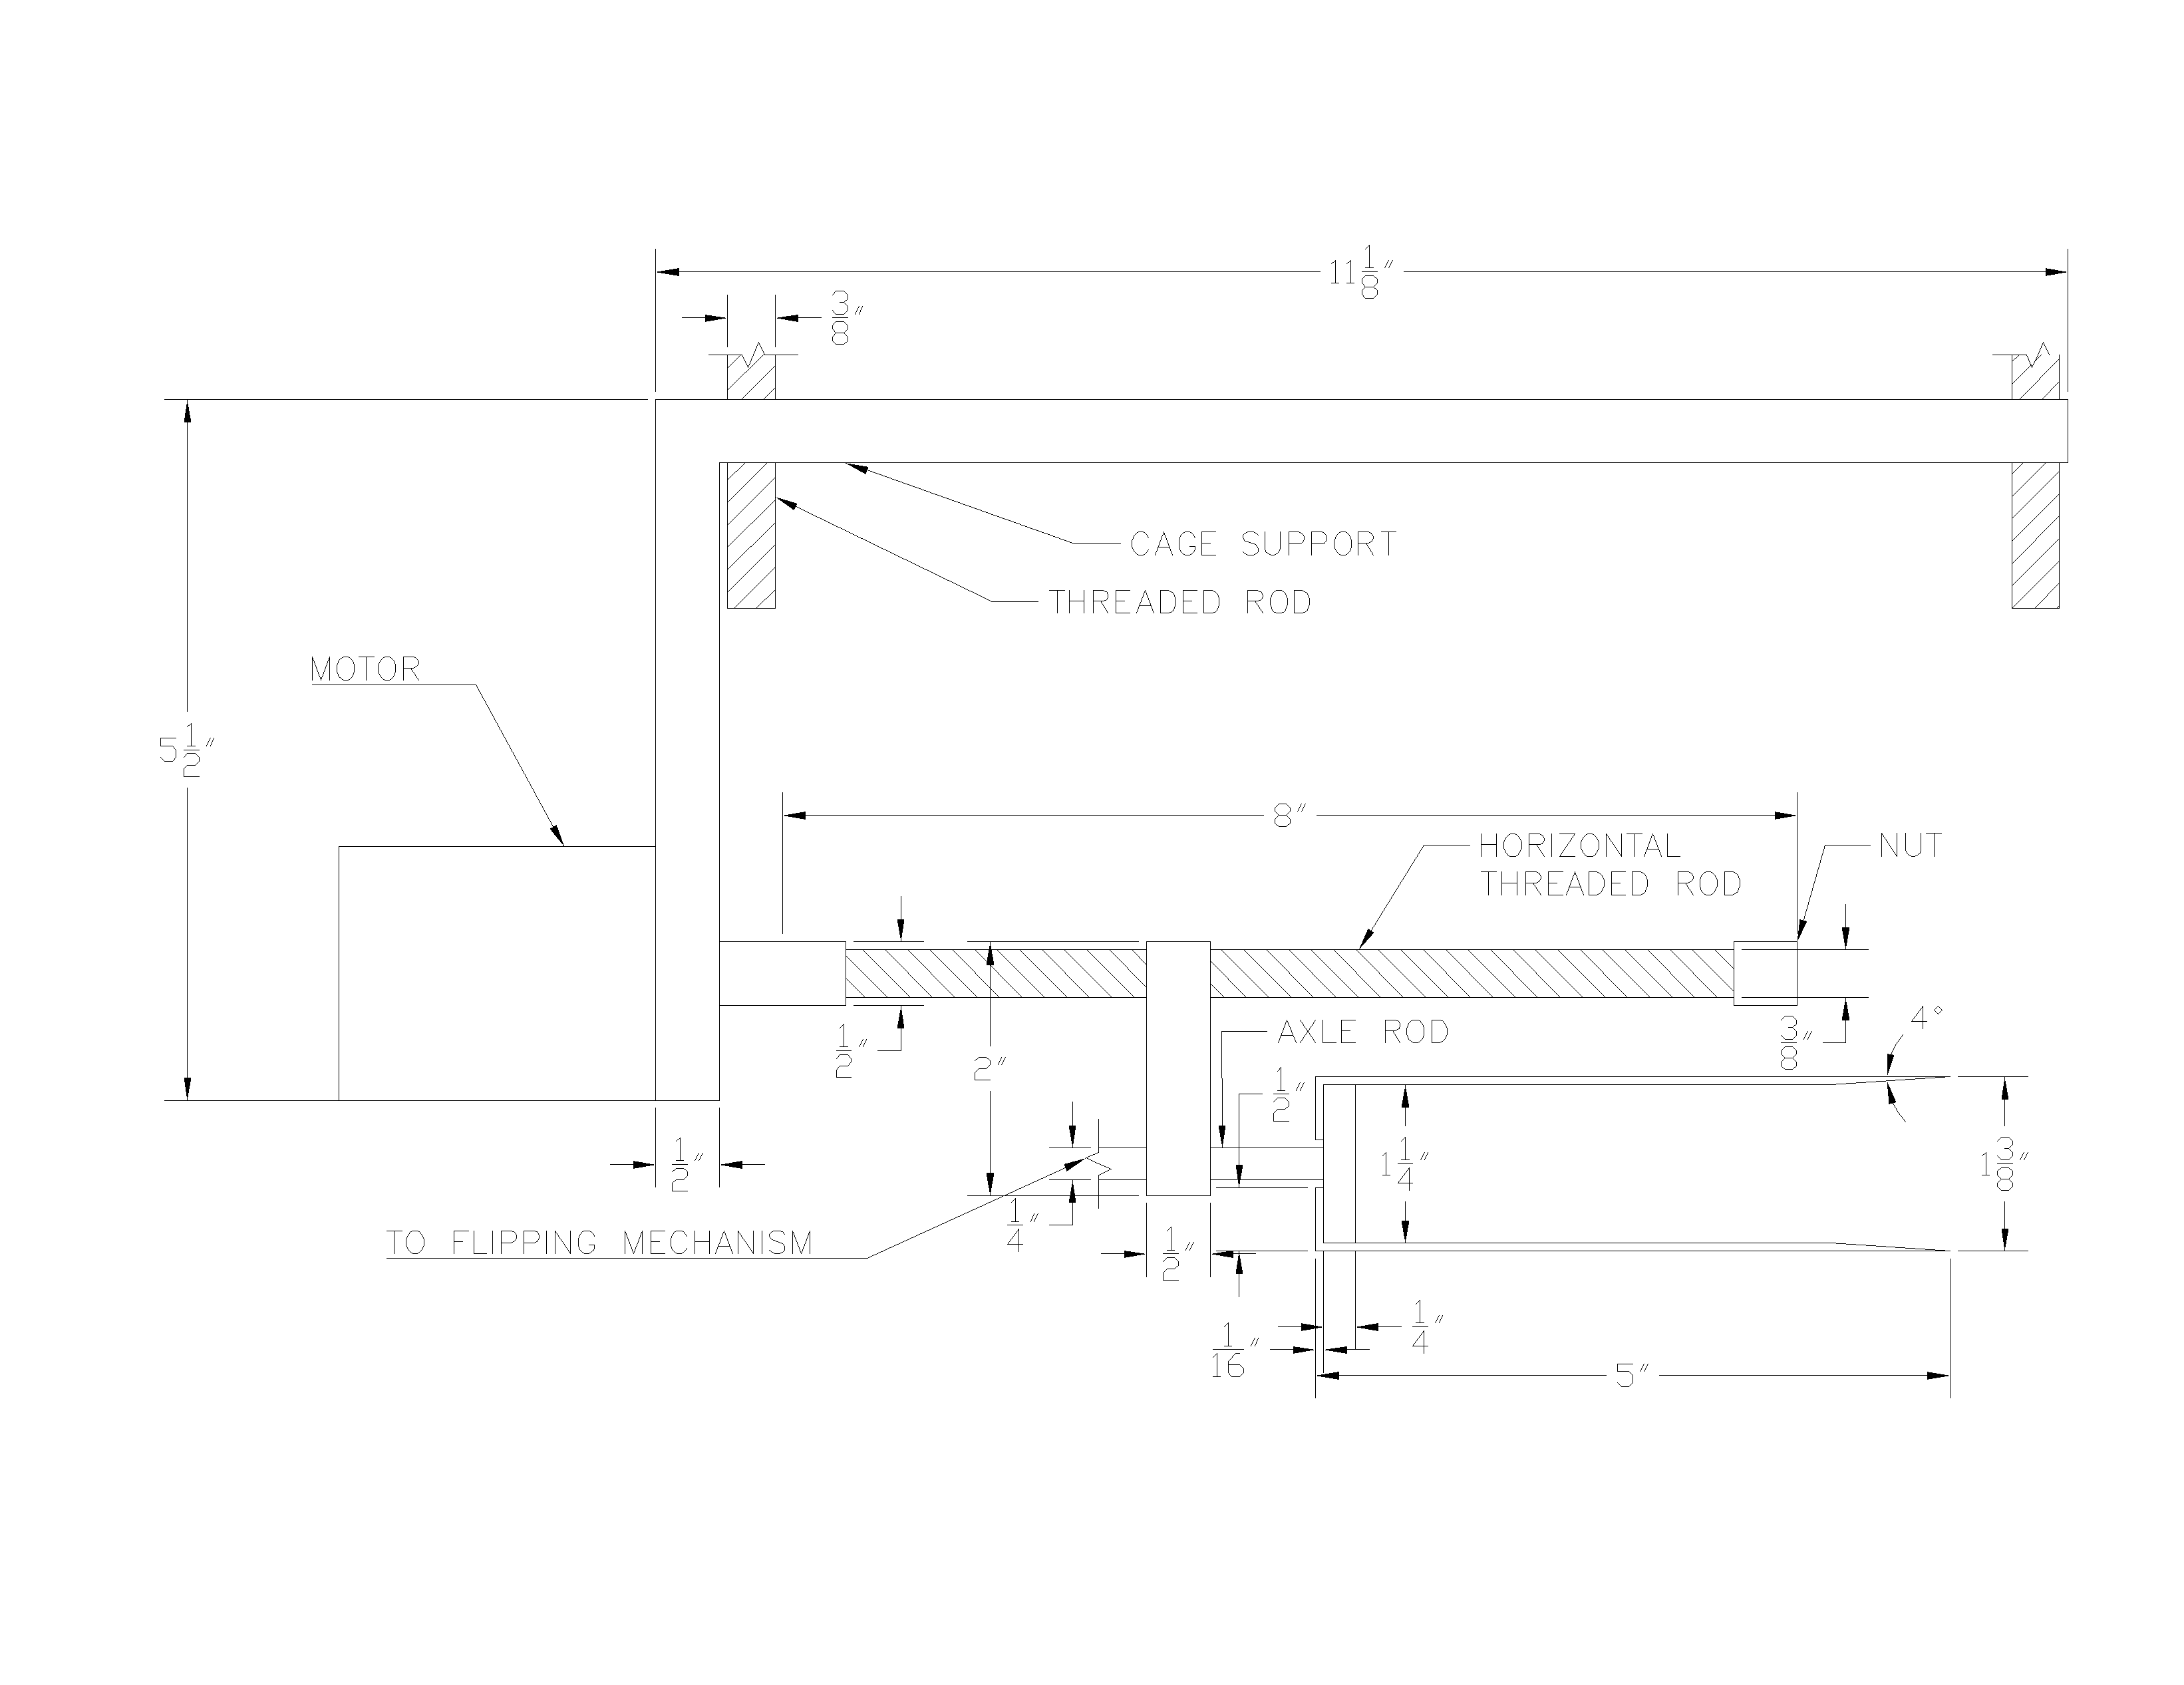
\includegraphics[width=0.6\linewidth]{res/spatula.png}
  \caption{The spatula design}
  \label{fig:spatula}
\end{figure}

The clamp component of the spatula is itself made of two metal plates and a coupling block.
Figure \ref{fig:spatula plate} shows the design of the plates.

\begin{figure}[H]
  \centering
  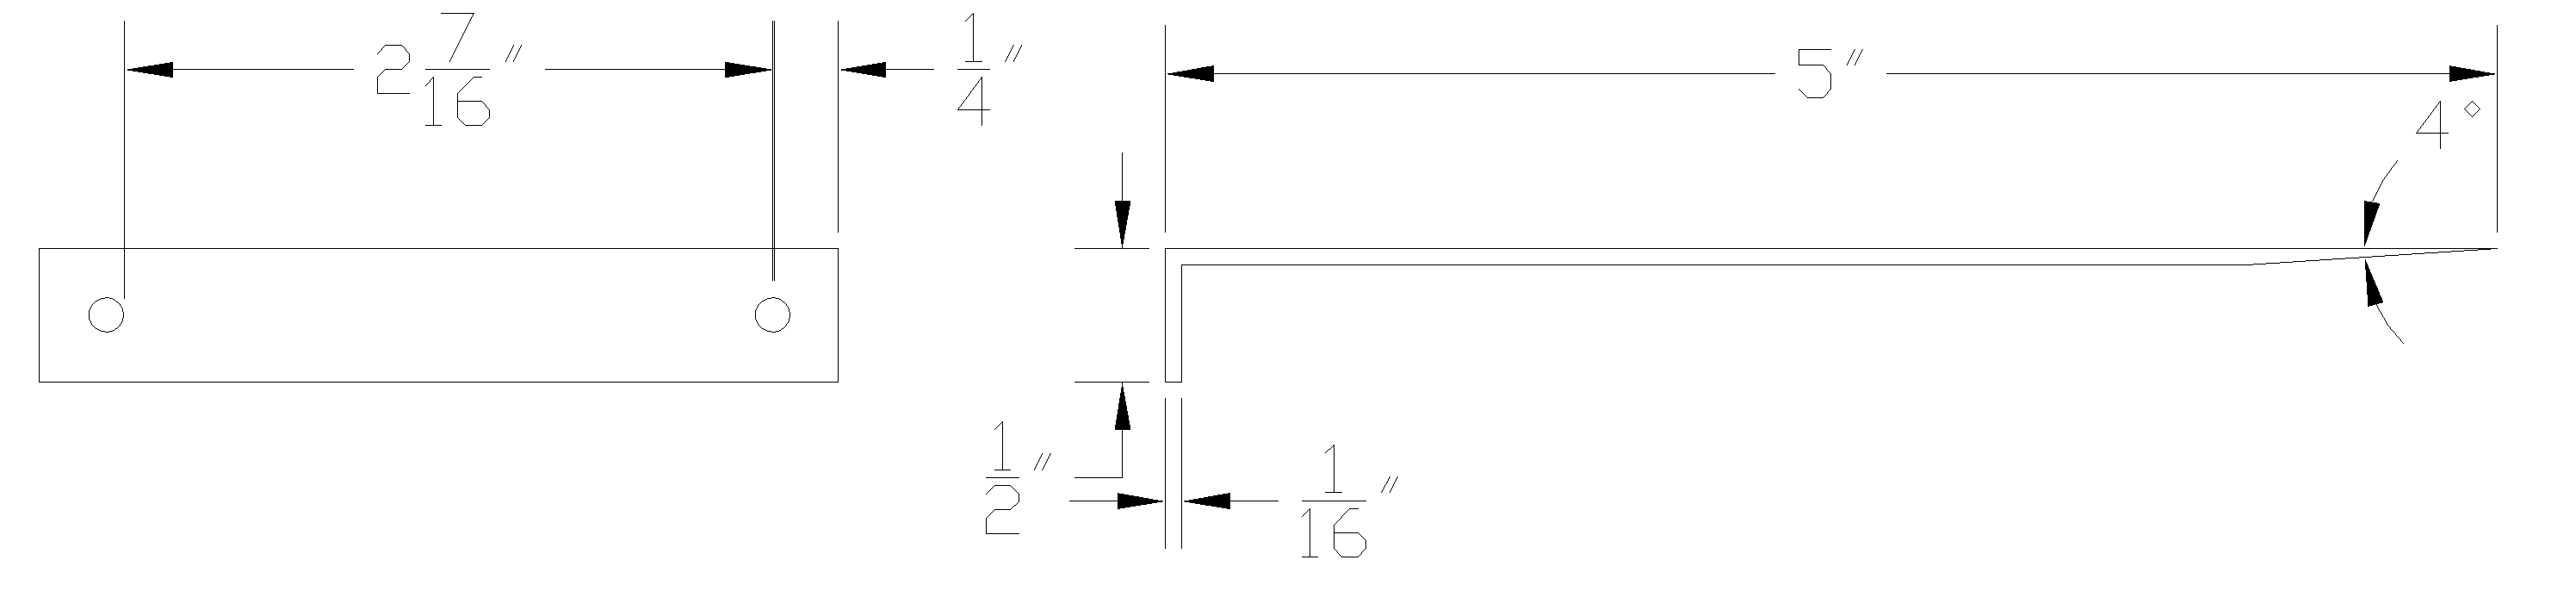
\includegraphics[width=0.6\linewidth]{res/spatula_plate.png}
  \caption{The plates from the spatula design}
  \label{fig:spatula plate}
\end{figure}

The plate is bent 90 \degree at one end, and two holes are drilled into this perpendicular edge.
These two plates are connected to each other and the rest of the device by a coupling block, which is shown in Figure \ref{fig:spatula coupling}.

\begin{figure}[H]
  \centering
  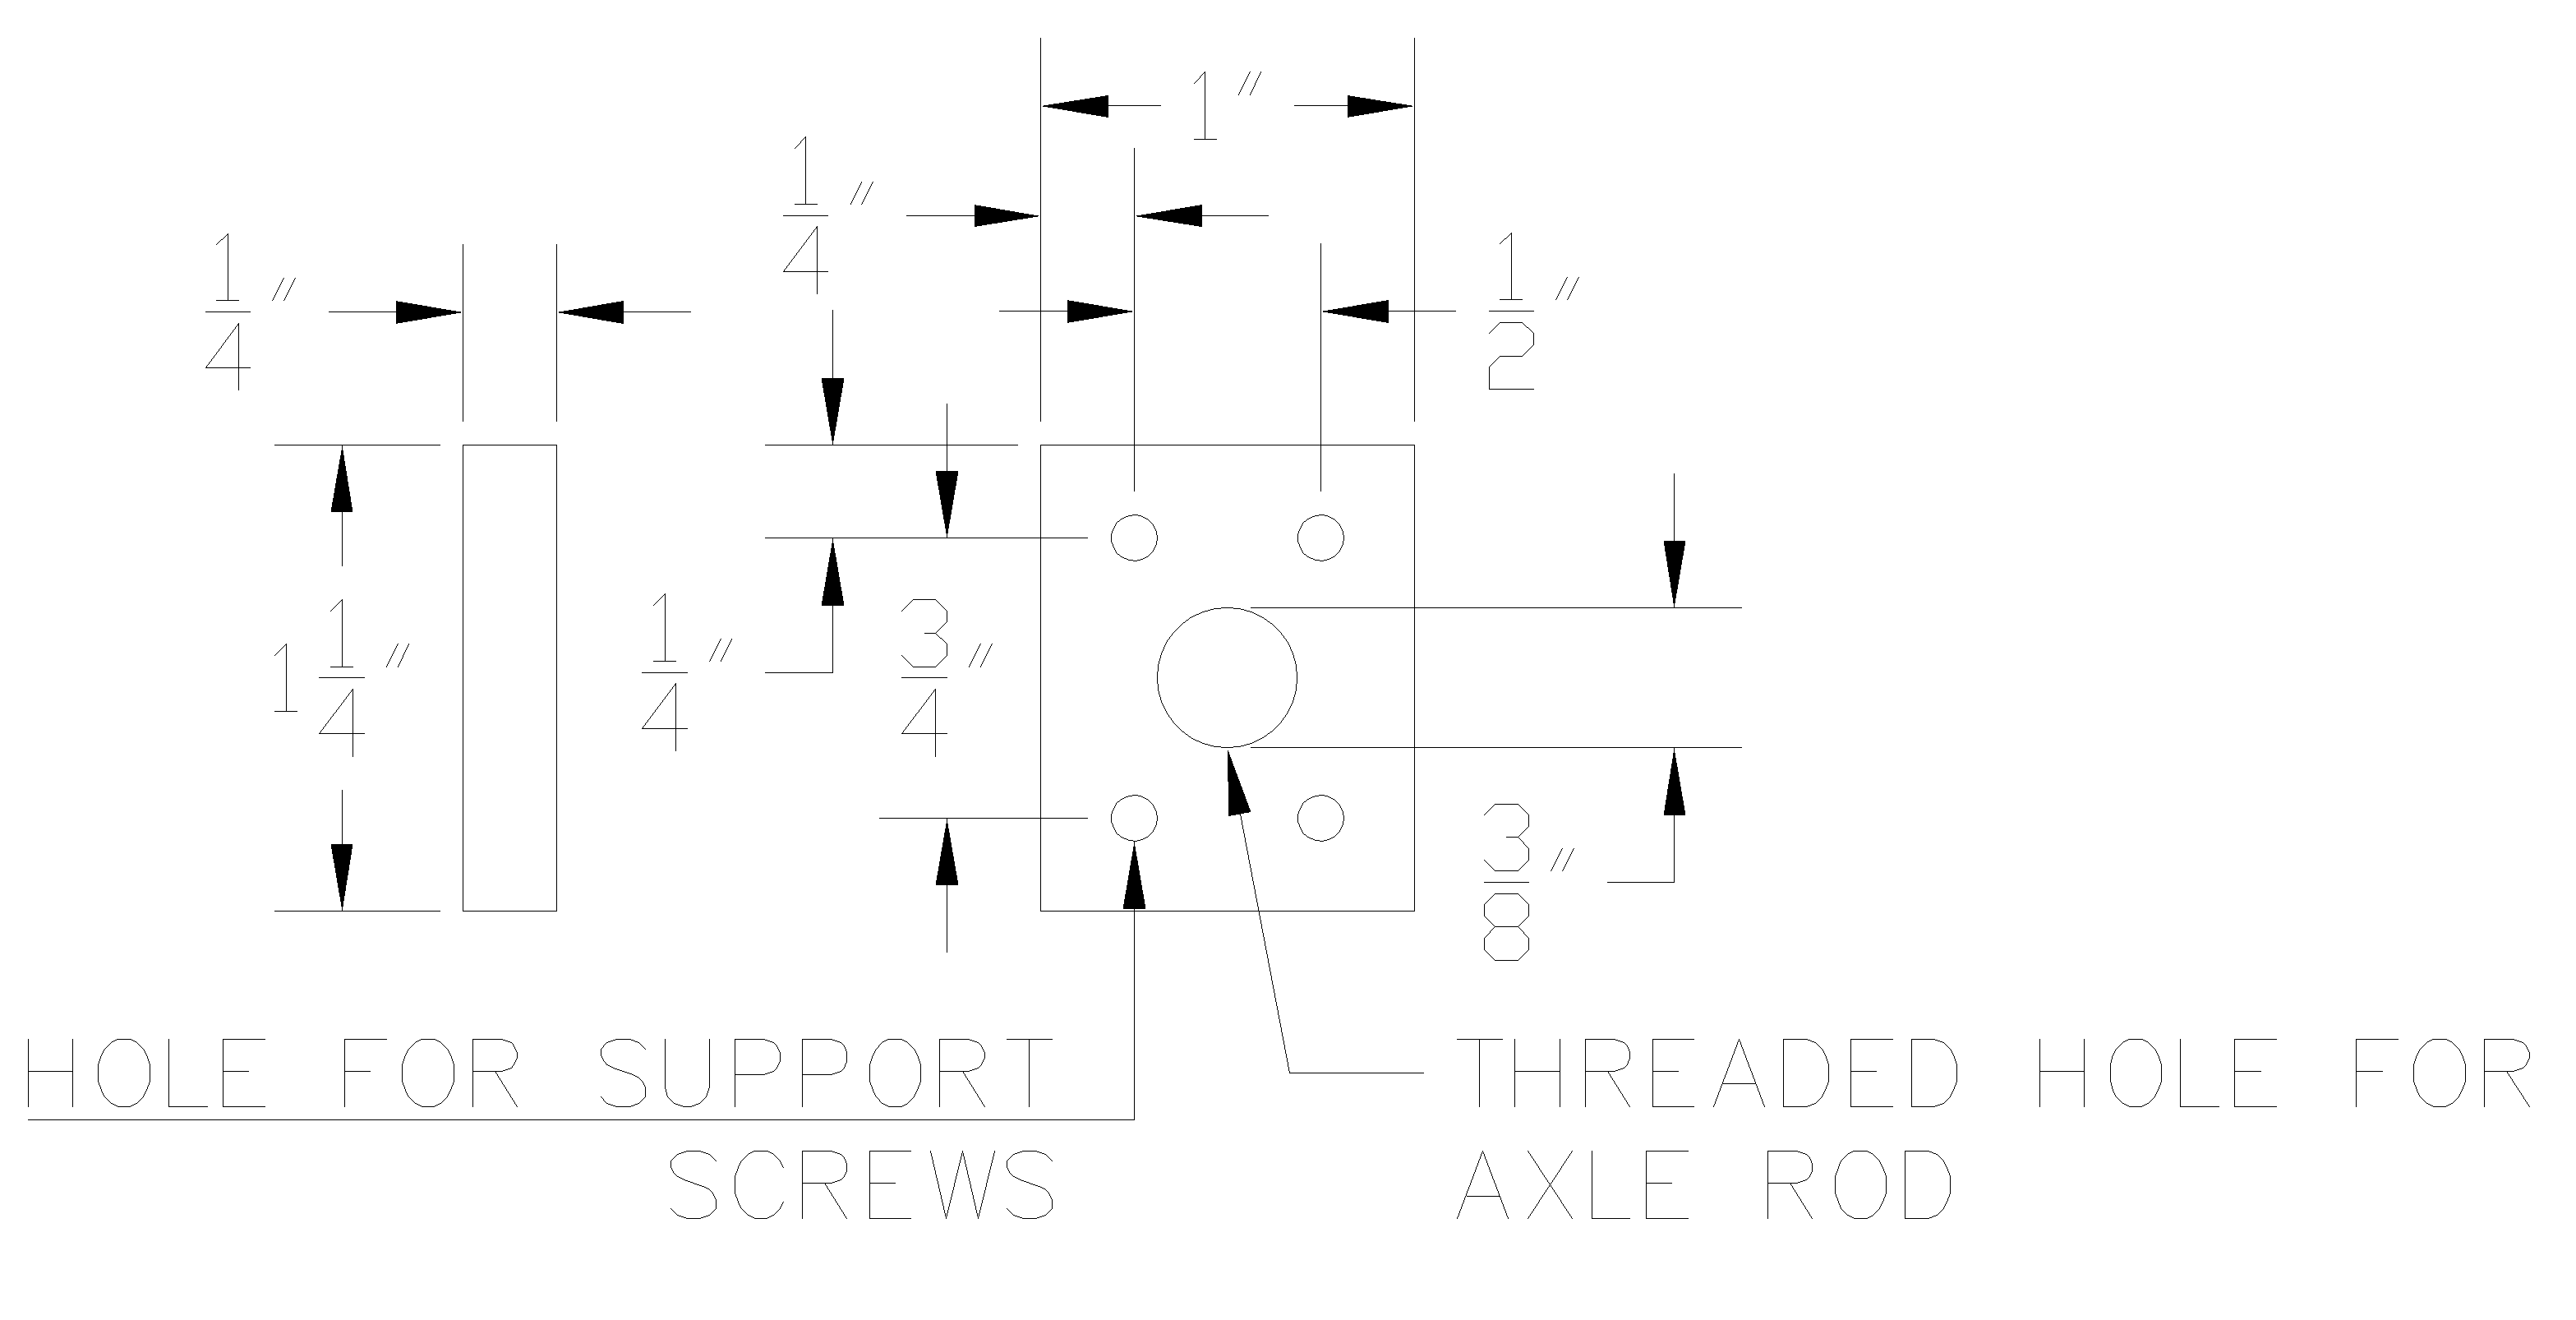
\includegraphics[width=0.6\linewidth]{res/spatula_coupling.png}
  \caption{The coupling from the spatula design}
  \label{fig:spatula coupling}
\end{figure}

The coupling block has five tapped holes drilled into it.
Four of the holes are used to screw the plates to the block, and the fifth is used to attach the rotational axle to it.

Another coupling block exists to connect the spatula clamp to the motor that drives the horizontal motion, shown in Figure \ref{fig:spatula horizontal coupling}.

\begin{figure}[H]
  \centering
  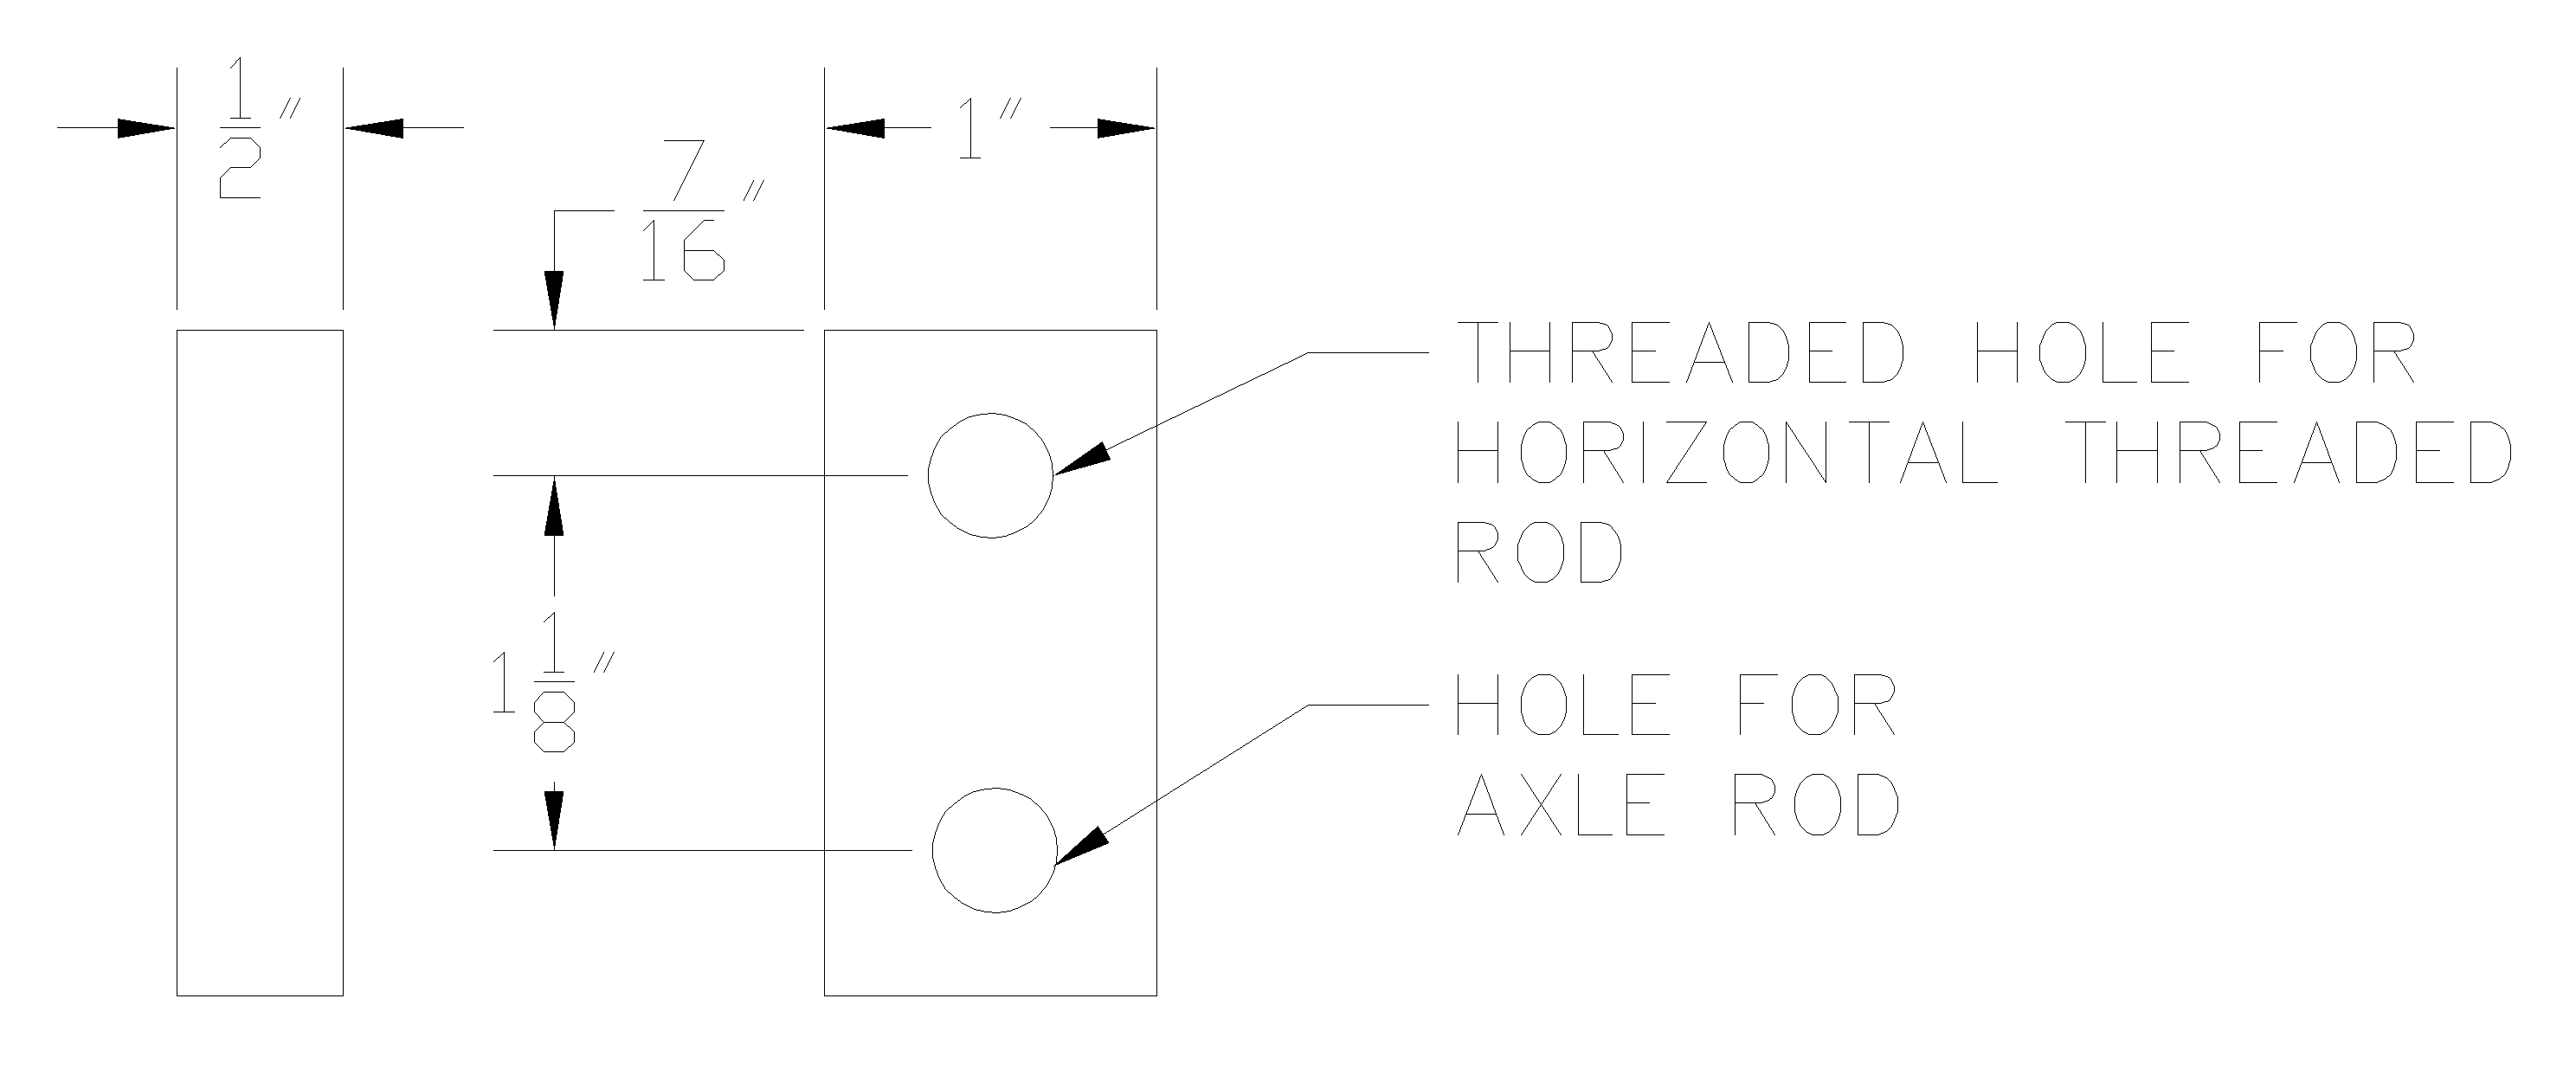
\includegraphics[width=0.6\linewidth]{res/spatula_horizontal_coupling.png}
  \caption{The horizontal coupling from the spatula design}
  \label{fig:spatula horizontal coupling}
\end{figure}

This coupling has a hole into which the ball screw drive fits, and a small hole at the other end through which the axle is passed.

Figure \ref{fig:spatula support} shows the coupling that attaches the spatula to the ball screws.

\begin{figure}[H]
  \centering
  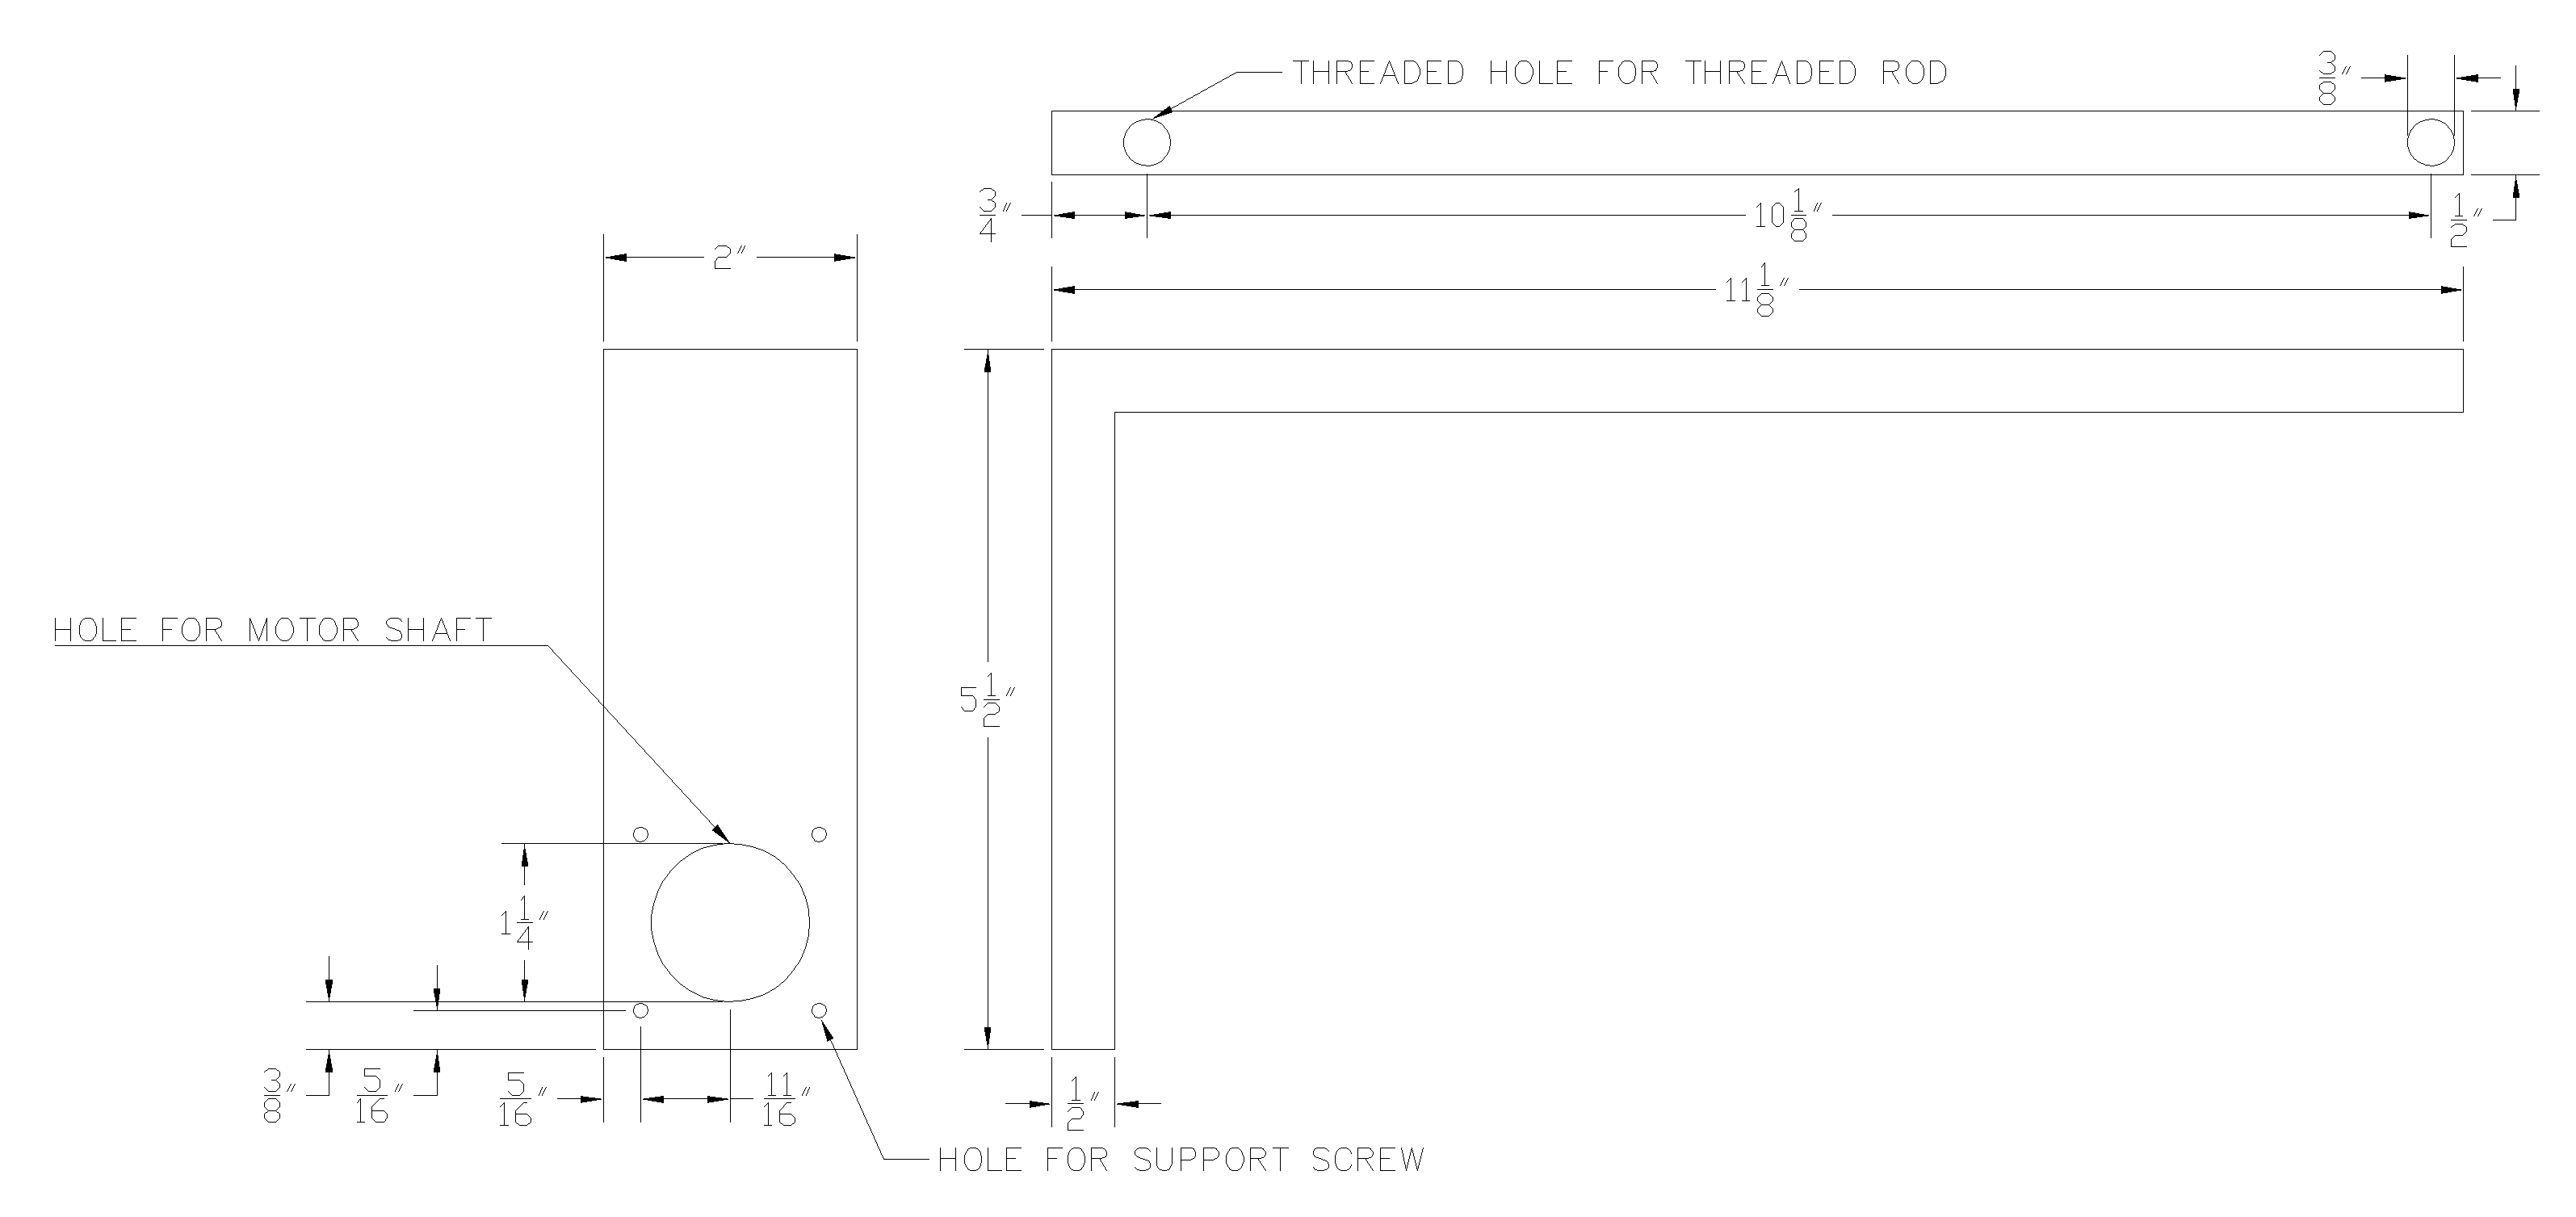
\includegraphics[width=0.6\linewidth]{res/spatula_support.png}
  \caption{The ball screw coupling from the spatula design}
  \label{fig:spatula support}
\end{figure}

The adapter has only one of the arms that extend downwards towards the pan.
At the end of this arm three holes are drilled.
The centre hole is sized for the shaft of the motor, and the other two holes are used to connect the motor to the adapter.
Another ball screw is coupled to the shaft of this motor, which is used to drive the horizontal motion of the spatula.

\subsubsubsection{Evaluation of Designs}

\noindent
The first criterion that is considered is the impact each candidate design has on the sear of the steak based on the outlined method for evaluation.

The cage-based design has three wires that sit between the steak and the pan.
The wires are very thin, however, and certainly do not create marks that are greater than 10 \% of the surface area of the steak.
Therefore, the cage-based design receives a score of six.
The spatula-based design, on the other hand, completely releases the steak on to the pan.
The steak is allowed to develop a complete, unimpeded, and natural sear, as it would if it was being cooked by a chef.
The spatula-based design receives a perfect score of ten.
The mesh-based design creates only one distinct mark on the steak, but the pattern of this mark covers the entire surface of the steak.
The mesh-based design receives a score of zero.

The estimated fabrication times---to be used as approximations of complexity---are displayed in Table \ref{table:steak handling fabrication times} below.

\begin{table}[H]
\begin{tabularx}{\textwidth}{X r}

\hline

Component & Estimated Fabrication Time \\

\hline

6" Angle Beam x 2 & 6 \\
7" Angle Beam x 2 & 7 \\
Coupling x 2 & 5 \\
Axle x 2 & 1 \\
Adapter & 3 \\
Wiring & 1 \\

\hline

Cage & 20 \\

\hline

Stainless Steel Plate x 2 & 8 \\
Plate Coupling & 4 \\
Horizontal Coupling & 4 \\
Axle & 1 \\
Adapter & 3 \\

\hline

Spatula & 20 \\

\hline

6" Angle Beam x 2 & 4 \\
7" Angle Beam x 2 & 4 \\
Coupling x 2 & 5 \\
Axle x 2 & 1 \\
Adapter & 3 \\
Mesh & 3 \\

\hline

Mesh & 20 \\

\hline

\end{tabularx}
\caption{Estimated fabrication times for the steak handling apparatus}
\label{table:steak handling fabrication times}
\end{table}

Table \ref{table:steak handling apparatus materials} below shows the costs, shipping times, and weights for the three candidate designs.

\begin{table}[H]
\begin{tabularx}{\textwidth}{l l Z Z Z Z Z}

\hline

Component & Source & Shipping Times & Cost & Volume ($ m^3 $) & Density ($ \frac{kg}{m^3} $) & Mass (kg) \\

\hline

Stainless Steel Sheet & Engineering Machine Shop & 0 & 5.30 & $250*10^{-6}$ & 7800 \cite{densities} & 1.95 \\
Stainless Steel Block & Engineering Machine Shop & 0 & 0.21 & $10*10^{-6}$ & 7800 \cite{densities} & 0.078 \\
Stainless Steel Rod & Engineering Machine Shop & 0 & 0.82 & $39*10^{-6}$ & 7800 \cite{densities} & 0.30 \\
Stainless Steel Wire & Engineering Machine Shop & 0 & 0.0023 & $0.11*10^{-6}$ & 7800 \cite{densities} & 0.00086 \\

\hline

Cage & & 0 & 6.30 & & & 2.3 \\

\hline

Stainless Steel Sheet & Engineering Machine Shop & 0 & 6.5 & $310*10^{-6}$ & 7800 \cite{densities} & 2.4 \\
Stainless Steel Block & Engineering Machine Shop & 0 & 0.046 & $2.2*10^{-6}$ & 7800 \cite{densities} & 0.017 \\
Ball Screw & Bearings Canada \cite{ballscrew} & 5 & 64.70 \cite{ballscrew} & $ 201 * 10^{-6} $ & 2700 \cite{densities} & 1.6 \\

\hline

Spatula & & 5 & 71 & & & 4.0 \\

\hline

Stainless Steel Sheet & Engineering Machine Shop & 0 & 5.3 & $250*10^{-6}$ & 7800 \cite{densities} & 1.95 \\
Stainless Steel Block & Engineering Machine Shop & 0 & 0.21 & $10*10^{-6}$ & 7800 \cite{densities} & 0.078 \\
Stainless Steel Rod & Engineering Machine Shop & 0 & 0.82 & $39*10^{-6}$ & 7800 \cite{densities} & 0.30 \\
Stainless Steel Mesh & Engineering Machine Shop & 0 & 0.040 & $1.9*10^{-6}$ & 7800 \cite{densities} & 0.015 \\

\hline

Mesh & & 5 & 6.40 & & & 2.3 \\

\hline

\end{tabularx}
\caption{Material and component details for the steak handling apparatus}
\label{table:steak handling apparatus materials}
\end{table}

The last criterion for the computational decision matrix is cleanability.
Cleanability is difficult to assess quantitatively.
To do so properly would require prototypes of each design, and sophisticated machinery that could measure the presence and quantity of trace particulates left on the components after a controlled cleaning cycle.
The design team does not possess the resources to carry out these tests, and so the best that can be done is a reasoned estimate of cleanability.

The spatula-based design is fairly modular, and free of textured surfaces in which food can stick.
If the plates are unscrewed from their couplings, the user is left with two flat, polished pieces of stainless steel.
These plates should be very simple to clean.
The cleaning time for the spatula-based design is estimated to be 5 minutes, with most of the time being taken up by the detachment and reattachment of the plates.

The caged-based design is as modular as the spatula-based design, but features a less-straightforward component to clean.
The wires are not as simple to scrub as the plates from the spatula-based design, and the bolted corners of the baskets present several crevices in which food can become lodged.
The cleaning time for the cage-based design is estimated to be 8 minutes.

Once again, the mesh-based design is modular.
It possesses the same bolted corners as the cage-based design, but replaces the wires with a tightly patterned stainless steel mesh.
The mesh presents great difficulty to effective cleaning.
It can be extremely difficult to remove greasy fats or tough fibres that become entangled.
The cleaning time for the mesh-based design is estimated to be 12 minutes.

Table \ref{table:steak handling apparatus matrix} shows the computational decision matrix.

\begin{table}[H]
\begin{tabularx}{\textwidth}{m{5cm} r Z Z Z Z Z Z Z Z Z}
  \hline
  & & \multicolumn{3}{c}{Cage} & \multicolumn{3}{c}{Spatula} & \multicolumn{3}{c}{Mesh} \\ 
  Criterion & Weight & S & N & W & S & N & W & S & N & W \\

  \hline

  Impact on sear & 20 & 6 & 0.6 & 12 & 10 & 1 & 20 & 0 & 0 & 0 \\
  Consistency of location of steak in pan & 15 & 1 & 1 & 15 & 0 & 0 & 0 & 1 & 1 & 15 \\
  Estimated fabrication time & 25 & $ \frac{1}{20} $ & 1 & 25 & $ \frac{1}{20} $ & 1 & 25 & $ \frac{1}{20} $ & 1 & 25 \\
  Cost & 15 & $\frac{1}{6.30}$ & 1 & 15 & $\frac{1}{71}$ & 0.089 & 1.3 & $\frac{1}{6.40}$ & 0.98 & 15 \\
  Shipping time & 5 & 5 & 1 & 5 & 0 & 0 & 0 & 5 & 1 & 5 \\
  Weight & 10 & $\frac{1}{2.3}$ & 1 & 10 & $\frac{1}{4.0}$ & 0.58 & 5.8 & $\frac{1}{2.3}$ & 1 & 10 \\
  Cleanability & 10 & $ \frac{1}{8} $ & 0.625 & 6.25 & $ \frac{1}{5} $ & 1 & 10  & $ \frac{1}{12} $ & 0.417 & 4.17 \\

  \hline

  \multicolumn{5}{r}{88} & \multicolumn{3}{r}{62} & \multicolumn{3}{r}{74} \\

  \hline

\end{tabularx}
\caption{Computational decision matrix for the steak handling apparatus design}
\label{table:steak handling apparatus matrix}
\end{table}

The cage-based design is 19 \% better than the mesh-based design and 42 \% better than the spatula-based design.

\subsubsection{Rotation}

The rotation mechanism is the piece that actually rotates the cage-based steak handling apparatus.
The cage is attached to an axle that extends outwards.
This axle is used to connect the apparatus to the rotation component.

\subsubsubsection{Evaluation Criteria}

\noindent
The candidate designs are evaluated based on cost, weight, temperature resistance, expected lifespan, and complexity.
Table \ref{table:steak handling apparatus criteria} shows the criteria by which the steak handling apparatus is evaluated.

\begin{table}[H]
\begin{tabularx}{\textwidth}{X  r}

\hline

Criterion & Weight \\

\hline

Estimated fabrication time & 40 \\
Cost & 25 \\
Shipping time & 5 \\
Weight & 20 \\
Temperature resistance & 10 \\

\hline

\end{tabularx}
\caption{Steak handling apparatus design criteria}
\label{table:steak handling apparatus criteria}
\end{table}

Temperature resistance is relevant to this piece of the design because the mechanism is located close to the pan, and therefore is exposed to significant heat.
The temperature resistance is numerically represented by the maximum safe temperature under which each candidate design can safely operate, based on the materials that they contain.

\subsubsubsection{Overview of Candidate Designs}

Three candidate designs are considered for the rotation mechanism.
The candidates are a bevel gear-based design, a sprocket and chain-based design, and a belt-based design.

The bevel gear-based design shown in Figure \ref{fig:bevel gear} rotates the motion from the motor 90 \degree.
The sprocket and chain-based design shown in Figure \ref{fig:sprocket and chain} translates the motor to another location, adding freedom and flexibility to its placement.

\begin{figure}[H]
\centering
\begin{minipage}{.5\textwidth}
  \centering
  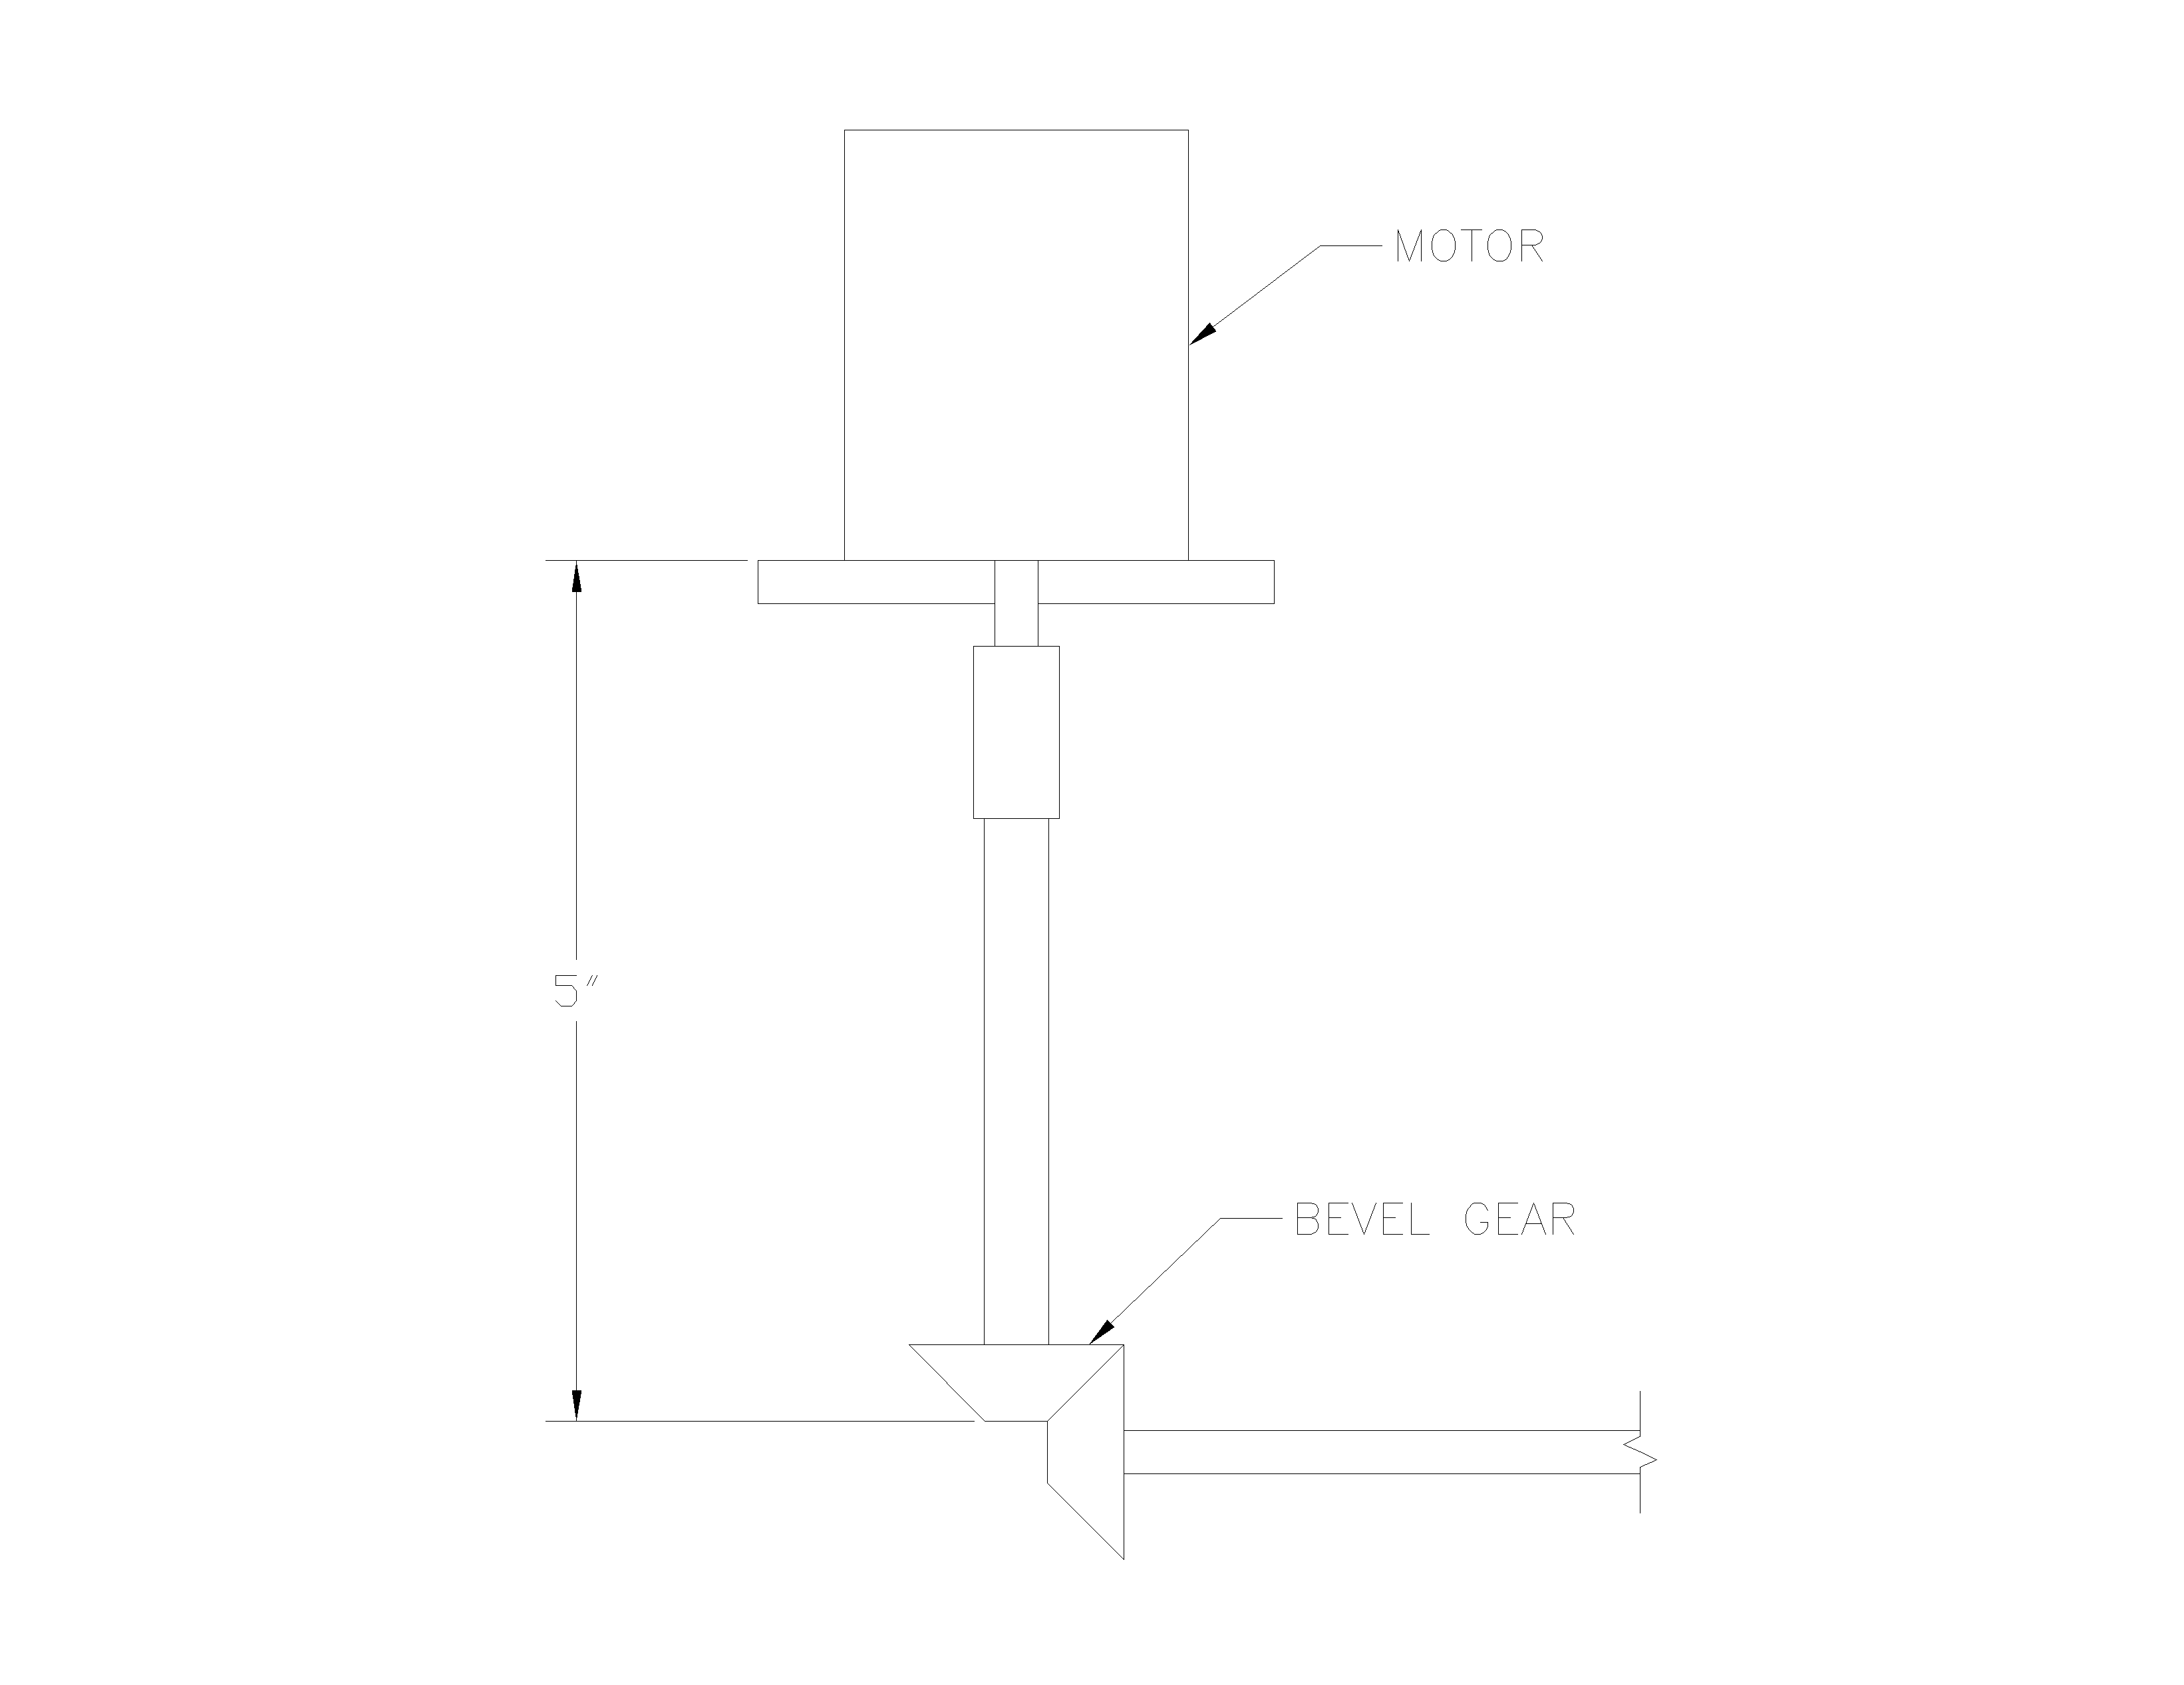
\includegraphics[width=\linewidth]{res/bevel_gear.png}
  \captionof{figure}{The bevel gear design}
  \label{fig:bevel gear}
\end{minipage}%
\begin{minipage}{.5\textwidth}
  \centering
  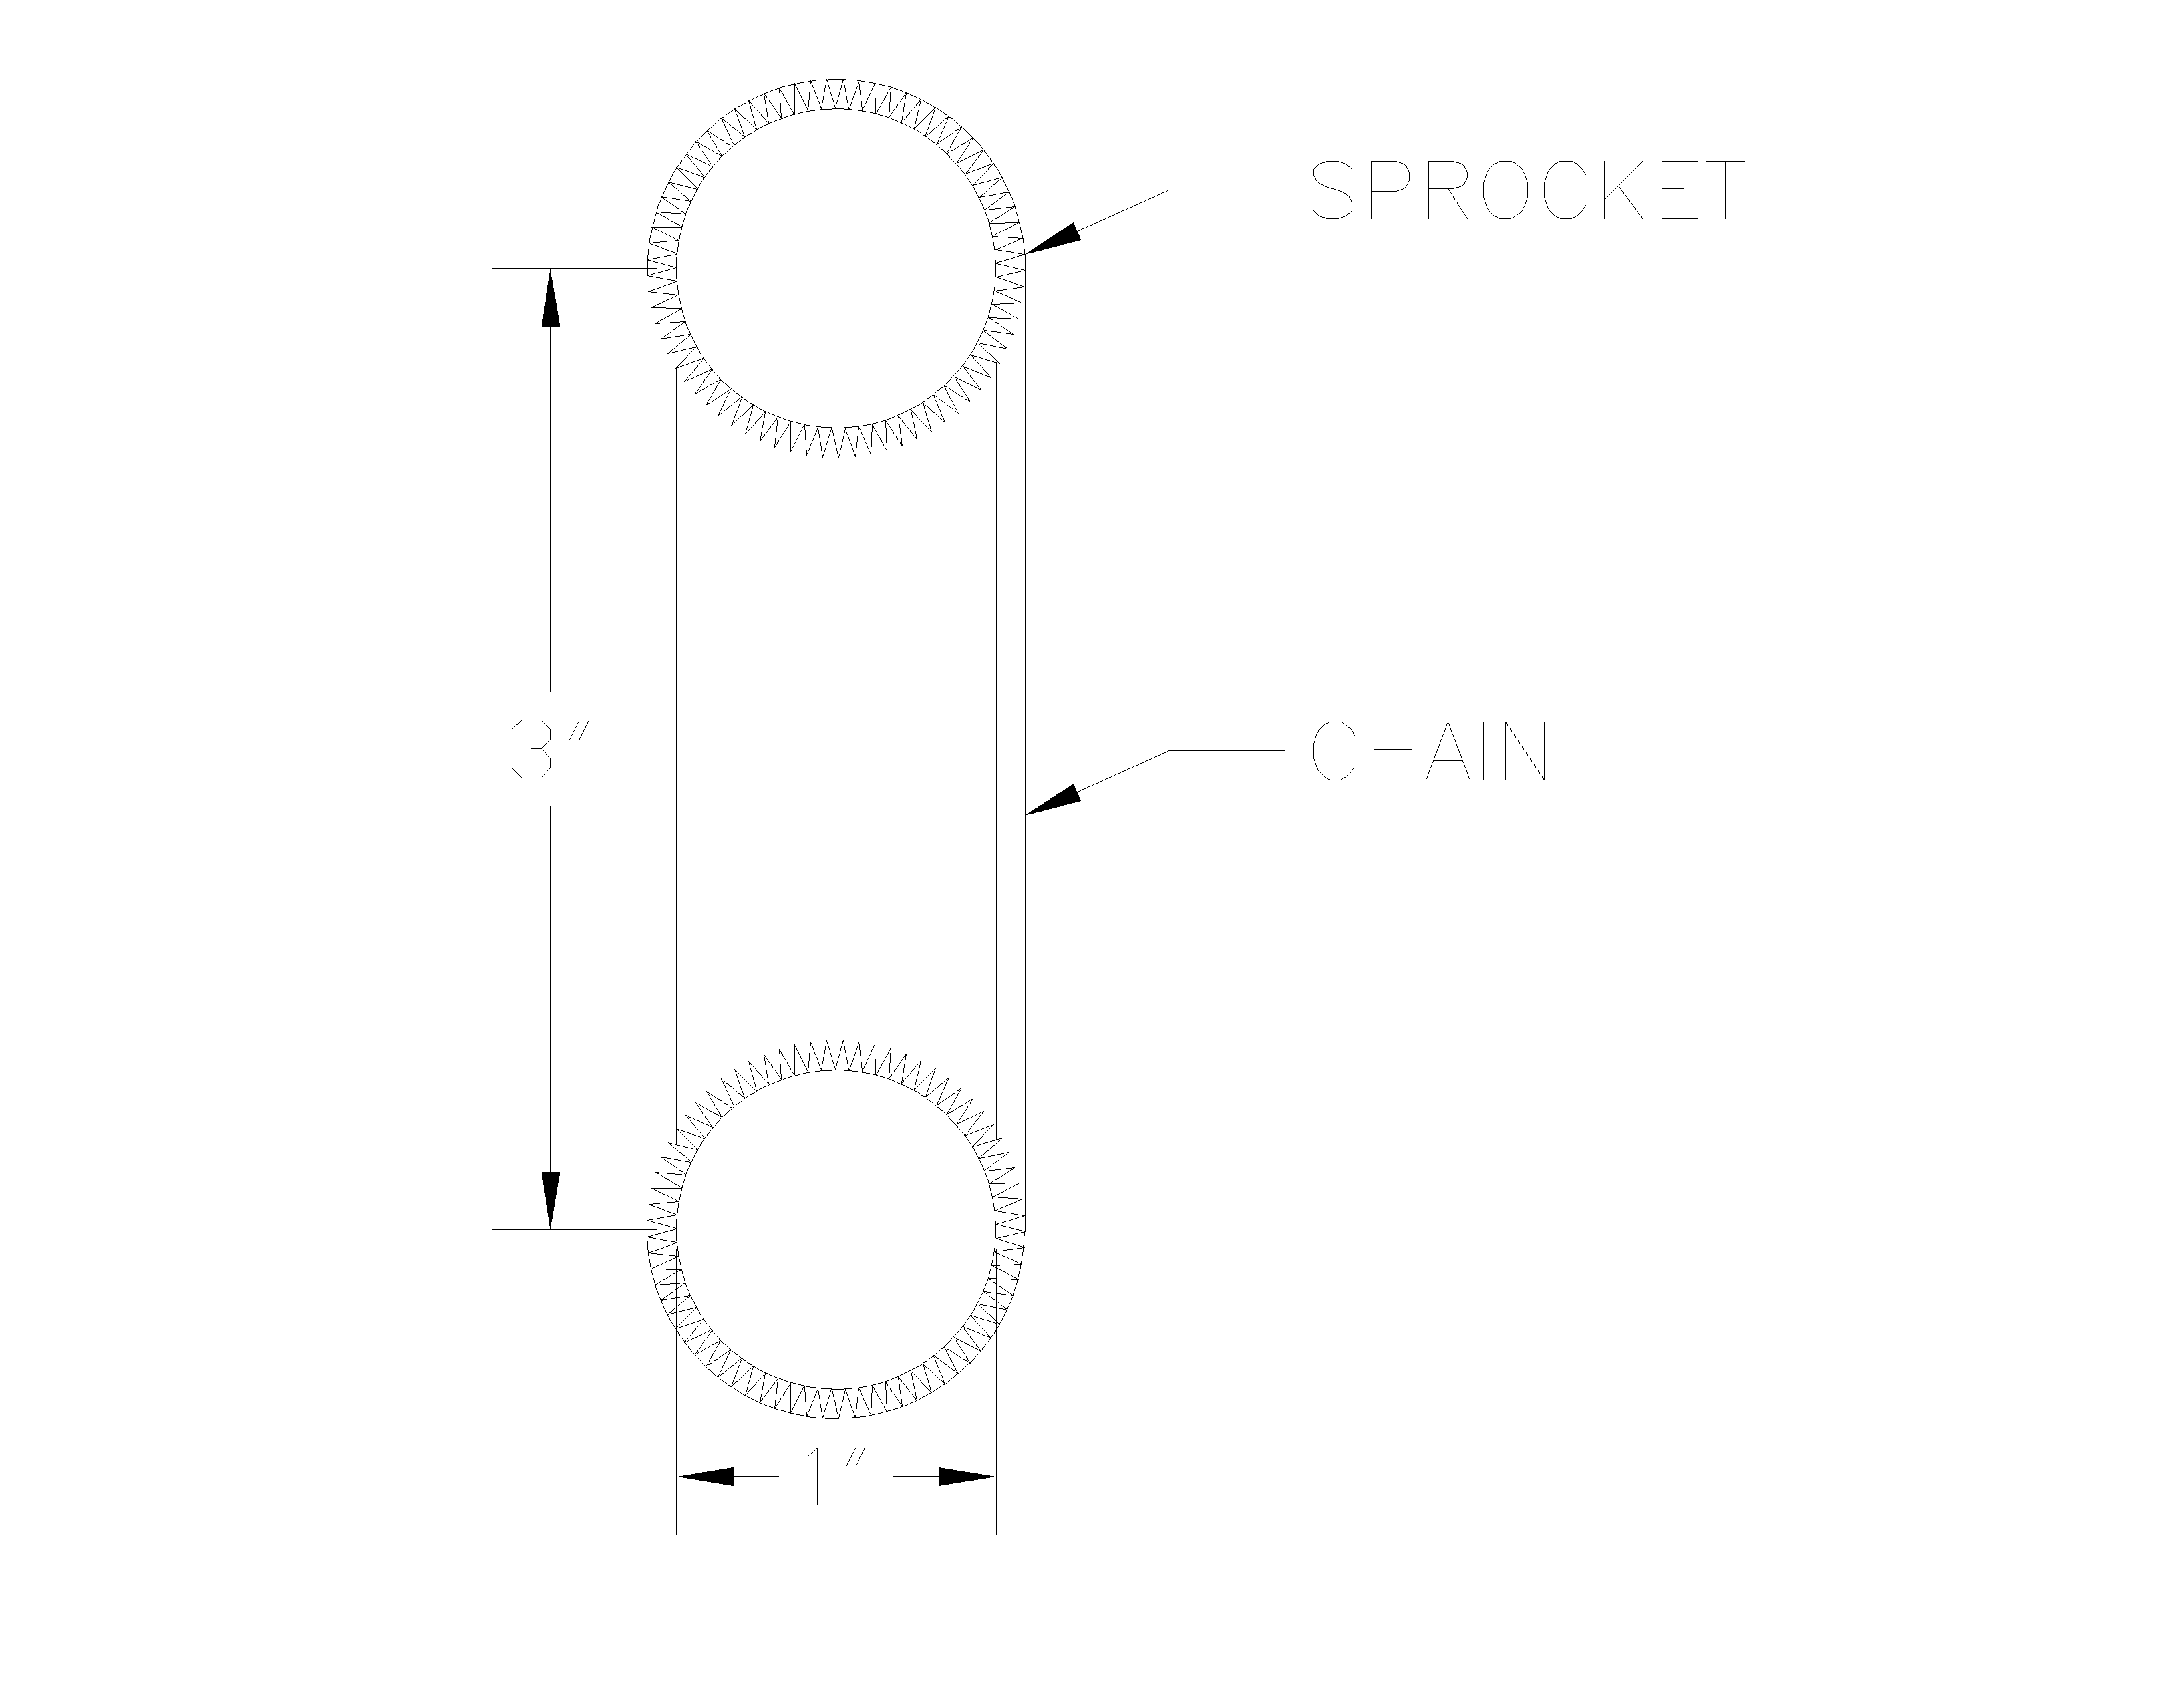
\includegraphics[width=\linewidth]{res/sprocket_and_chain.png}
  \captionof{figure}{The sprocket and chain design}
  \label{fig:sprocket and chain}
\end{minipage}
\end{figure}

Like the sprocket and chain-based design, the belt-based design in Figure \ref{fig:belt} frees the placement of the motor by translating its motion.

\begin{figure}[H]
  \centering
  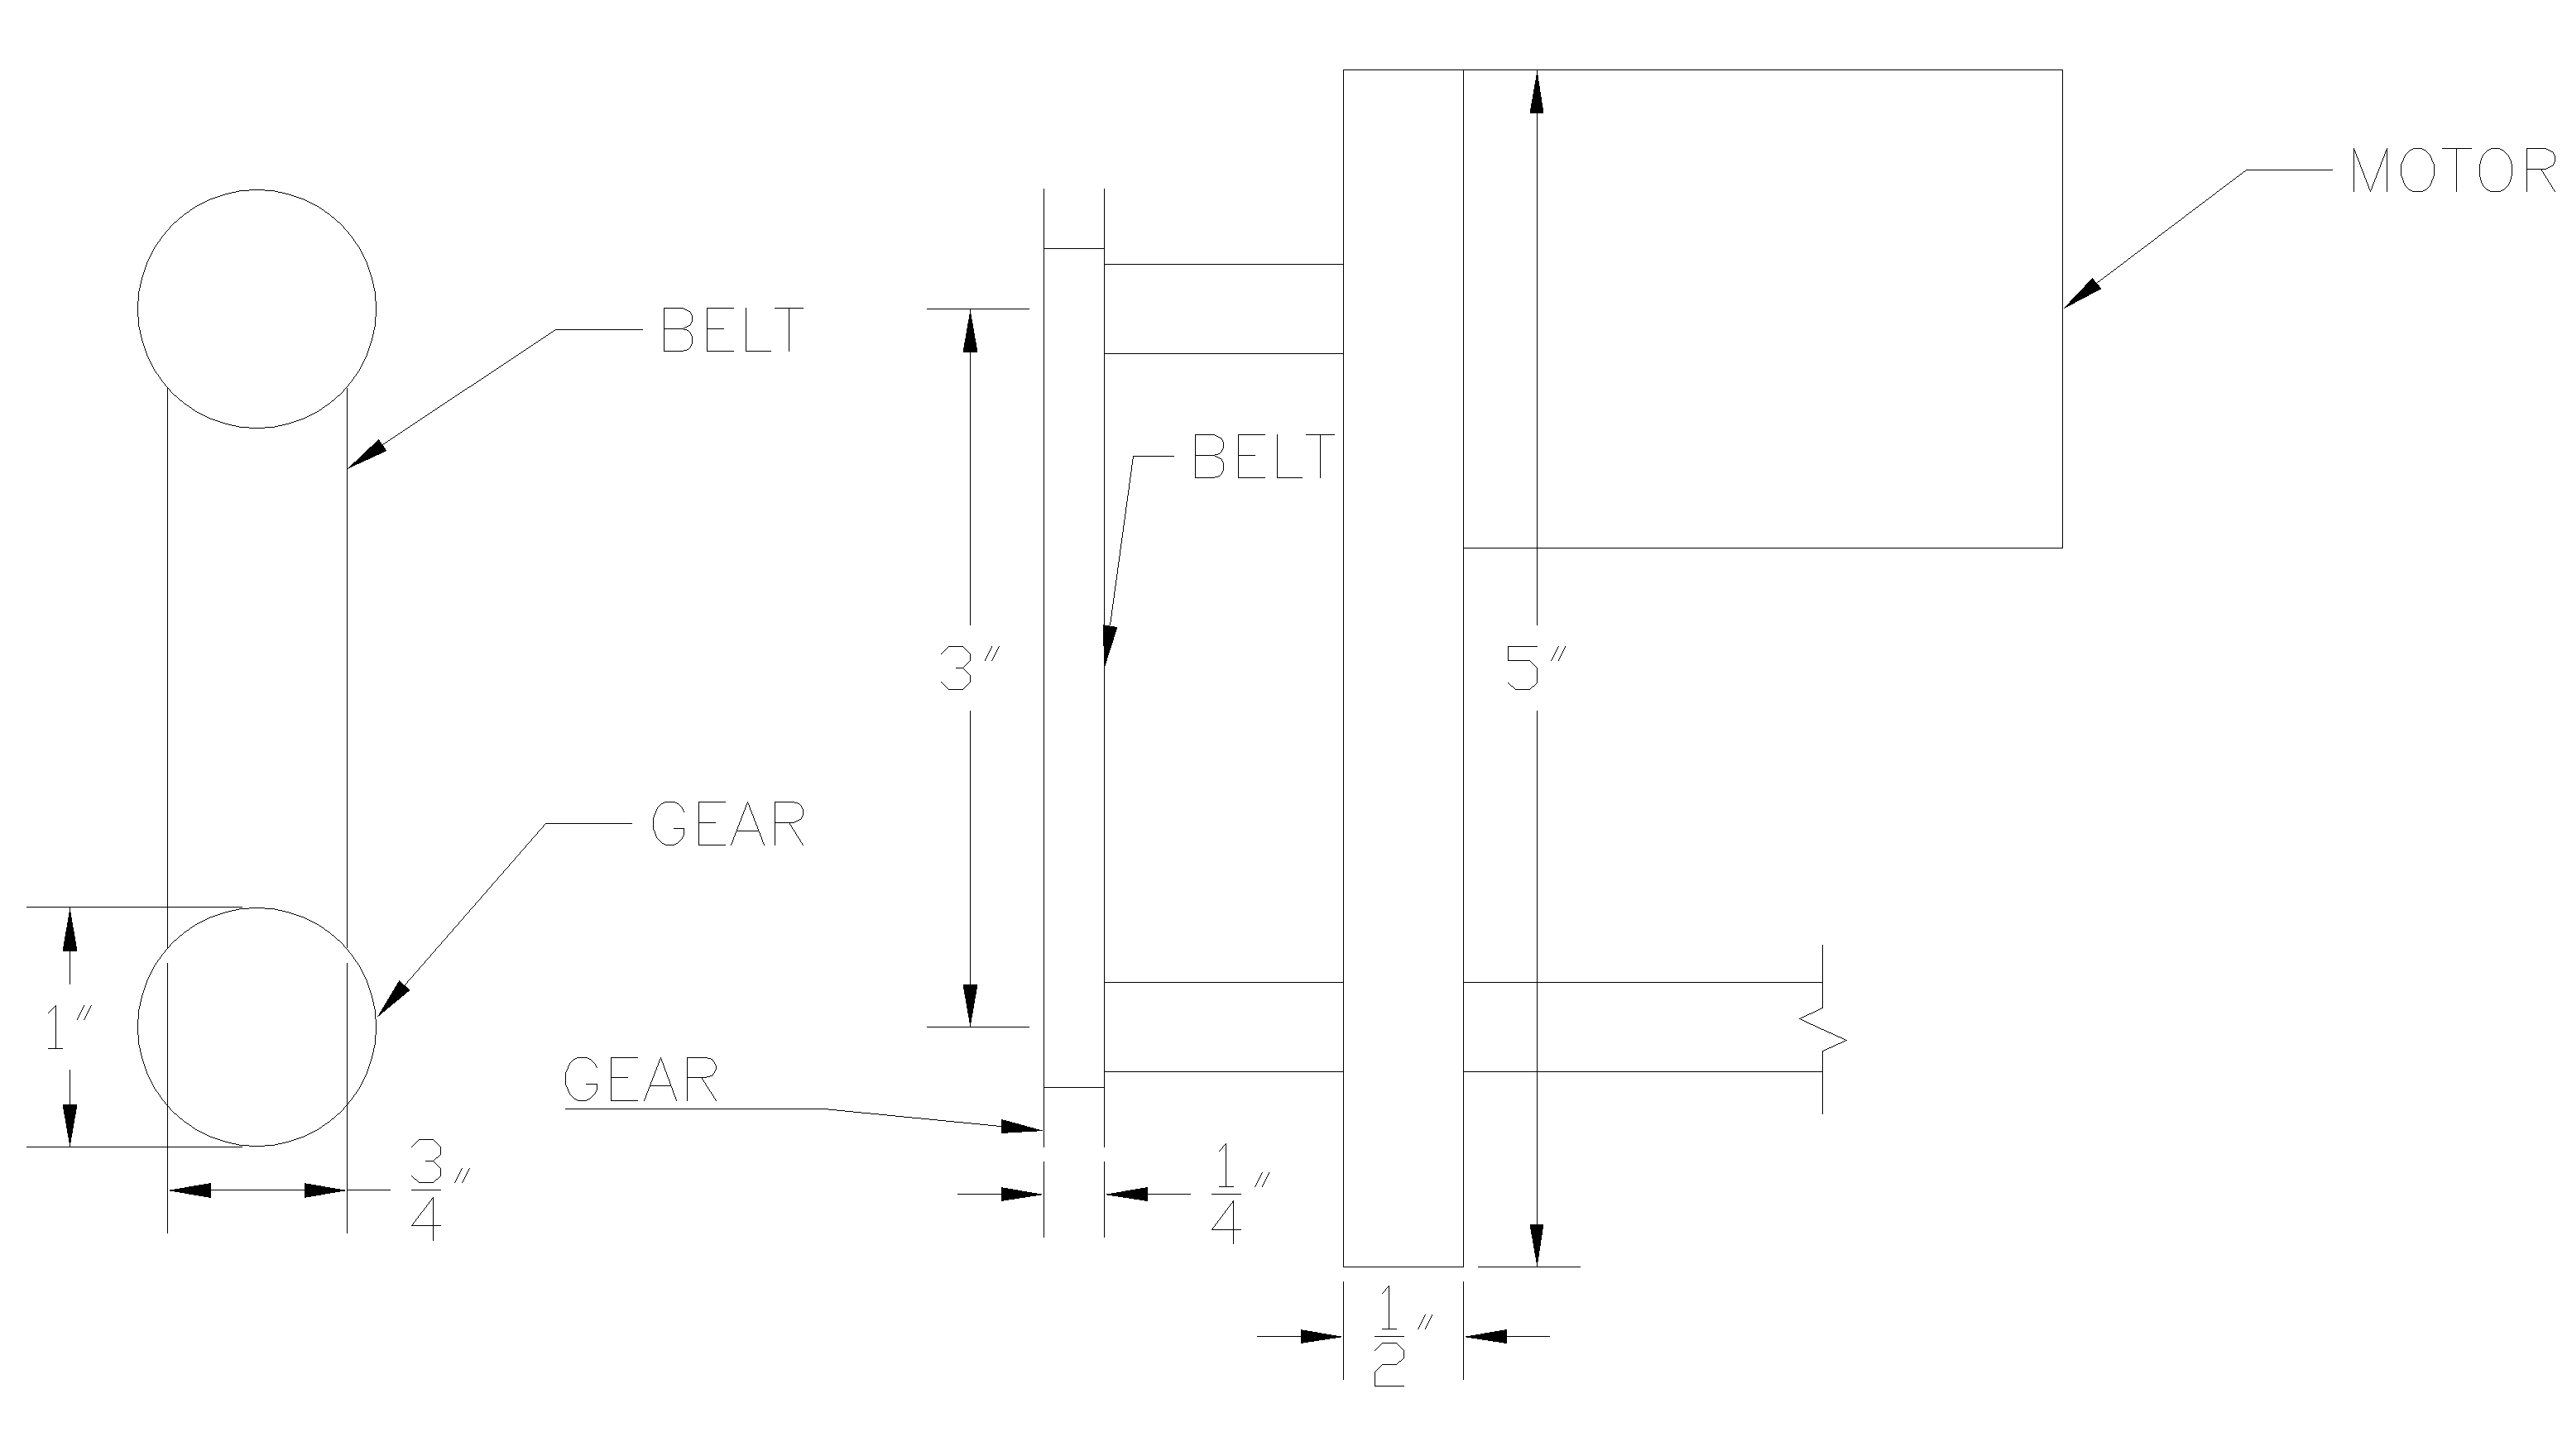
\includegraphics[width=0.6\linewidth]{res/belt.png}
  \caption{The belt design}
  \label{fig:belt}
\end{figure}

\subsubsubsection{Evaluation of Designs}

The bevel gear-based design allows the motor to be positioned perpendicular to the axle of rotation.
This is greatly beneficial, because it eliminates the need to cut a large circle out of the ball screw adapter.
Cutting into the stainless is steel is a slow and difficult process.
It also allows the motor to be placed on the exterior of the adapter’s u bend, saving valuable space in the rotation area of the cage, and decreasing the difficulty of the fabrication of the device.
It is estimated that fixing the gears to the axles and securing the motor would take twelve hours in total.

The sprocket and chain- and belt-based designs are very similar.
The only difference between the two is the method of transmission between the two axles; the fabrication work that needs to occur is the same.
Holes need to be drilled in one side of the adapter, alongside a large circular hole into which the motor slots.
It is estimated that the designs would each take twenty hours to implement.

Table \ref{table:rotation mechanism materials} below show the costs, shipping times, and weights for the three candidate designs.

\begin{table}[H]
\begin{tabularx}{\textwidth}{l l Z Z Z Z Z}

\hline

Component & Source & Shipping Times & Cost & Volume ($ m^3 $) & Density ($ \frac{kg}{m^3} $) & Mass (kg) \\

\hline

Bevel Gear x 2 & McMaster-Carr \cite{bevel} & 5 & \$ 30.40 \cite{bevel} & $ 5.43*10^{-6} $ \cite{bevel} & 7800 \cite{densities} & $ 42.4*10^{-3} $ \\

\hline

Bevel Gear & & 5 & \$ 60.08 & & & $ 84.8*10^{-3} $ \\

\hline

Sprocket x 2 & McMaster-Carr \cite{sprocket} & 5 & \$ 11.97 \cite{sprocket} & $ 4.93*10^{-6} $ \cite{sprocket} & 7800 \cite{sprocket} & $ 38.5*10^{-3} $ \\
Chain & McMaster-Carr \cite{chain} & 5 & \$ 6.53 \cite{chain} & $ 6.96*10^{-6} $ \cite{chain} & 7800 \cite{densities} & $ 54.3*10^{-3} $ \\

\hline

Sprocket and Chain & & 5 & \$ 30.47 & & & $ 131*10^{-3} $ \\

\hline

Belt & McMaster-Carr \cite{belt} & 5 & \$ 14.27 \cite{belt} & $ 9.83*10^{-6} $ \cite{belt} & 2300 \cite{silicone} & $ 22.6*10^{-3} $ \\
Belt Pulley x 2 & McMaster-Carr \cite{pulley} & 5 & \$ 15.10 \cite{pulley} & $ 0.116*10^{-6} $ \cite{pulley} & 7800 \cite{densities} & $ 0.90*10^{-3} $ \\

\hline

Belt & & 5 & \$ 44.47 & & & $ 24.4*10^{-3} $ \\

\hline

\end{tabularx}
\caption{Material and component details for the rotation mechanism}
\label{table:rotation mechanism materials}
\end{table}

The bevel gears are made of carbon steel, which has an estimated maximum safe operating temperature of 500 \degree C \cite{carbonsteel}.
Likewise, both the sprockets and the chain are made of carbon steel.
In the belt-based design, the belt itself experiences failure due to temperature far earlier than the steel pulleys.
The belt is rated for use in temperatures up to 205 \degree C \cite{belt}.

Table \ref{table:rotation matrix} shows the computational decision matrix.

\begin{table}[H]
\begin{tabularx}{\textwidth}{m{5cm} r Z Z Z Z Z Z Z Z Z}
  \hline
  & & \multicolumn{3}{c}{Bevel Gear} & \multicolumn{3}{c}{Sprocket and Chain} & \multicolumn{3}{c}{Belt} \\
  Criterion & Weight & S & N & W & S & N & W & S & N & W \\

  \hline

  Estimated fabrication time & 40 & $ \frac{1}{12} $ & 1 & 40 & $ \frac{1}{20} $ & 0.6 & 24 & $ \frac{1}{20} $ & 0.6 & 24 \\
  Cost & 25 & $ \frac{1}{60.08} $ & 0.506 & 12.65 & $ \frac{1}{30.47} $ & 1 & 25 & $ \frac{1}{44.47} $ & 0.686 & 17.2 \\
  Shipping time & 5 & $ \frac{1}{5} $ & 1 & 5 & $ \frac{1}{5} $ & 1 & 5 & $ \frac{1}{5} $ & 1 & 5 \\
  Weight & 20 & 11.8 & 0.29 & 5.8 & 7.60 & 0.185 & 3.7 & 41.0 & 1 & 20 \\
  Temperature resistance & 10 & 500 & 1 & 10 & 500 & 1 & 10 & 205 & 0.41 & 41 \\

  \hline

  \multicolumn{5}{r}{73.5} & \multicolumn{3}{r}{67.7} & \multicolumn{3}{r}{70.3} \\

  \hline

\end{tabularx}
\caption{Computational decision matrix for the rotation mechanism}
\label{table:rotation matrix}
\end{table}

The bevel gear-based design is 4.41 \% better than the belt-based design and 8.42 \% better than the sprocket and chain-based design.

\subsection{Sensory Subsystem}

This section outlines the design of the sensory subsystem, the subsystem that monitors the conditions that are relevant to the cooking of the steak.

\subsubsection{Evaluation Criteria}

Table \ref{table:sensory criteria} shows the criteria by which the sensory designs are evaluated.

\begin{table}[H]
\begin{tabularx}{\textwidth}{X  r}

\hline

Criterion & Weight \\

\hline

Ease of electrical implementation & 30 \\
Ease of mechanical implementation & 30 \\
Quality of cooked steak & 20 \\
Reliability & 20 \\

\hline

\end{tabularx}
\caption{Sensory design criteria}
\label{table:sensory criteria}
\end{table}

The sensor needs to be easily incorporated into the overall system and should not be in the way, which is reflected in the ease of electrical and mechanical implementation criteria.
Ease of electrical implementation refers to the cost and ease of electrically implementing the sensors within the system.
For example, positioning the sensors directly on the steak places them in close proximity the the heat source, which complicates the electrical design and adds cost.

Likewise, ease of mechanical implementation refers to whether or not the sensor placement interferes with the current mechanical design, thereby requiring more consideration and potential design revisions.
Due to the cost of the electrical and mechanical implementations, in terms of both time and monetary costs, they have been assigned equal weightings of 30\%.

Quality of cooked steak refers to the visual aesthetic and appeal of the steak, and the whether the sensor placement could potentially negatively impact it.
Reliability is in reference to the lifespan of the sensor.
Both have been assigned lower weightings of 20\%, as they are not as critical in the sensory subsystem design as the actual implementation is. 

Finally, any sensor considered needs to be able to measure up to 300 \degree C for the temperature of the pan, and accurately monitor temperatures up to 71 \degree C with an error range of 1.5 \degree C, as per the functional specifications discussed in Table \ref{table:func spec}. 

\subsubsection{Overview of Candidate Designs}

The potential solutions considered for the sensory subsystem are listed as follows: sensors intermeshed with the cage, sensor rod acting as a spit, Infrared (IR) thermometer, and IR thermometer and sensor rod together.

The first design considered is to interlace the sensors into the threaded cage strands.
The wiring would then be routed back up to the microcontroller.
Types of sensors that fulfill this sort of application are thermistors or thermocouples.

NTC thermistors work by displaying changes in resistor proportional to changes in temperature.
Their effective operating range is between -50 \degree C to 250 \degree C for standard thermistors.
To choose a thermistor for a particular application, calculations are necessary with the thermistor beta formula \cite{se1}.
Due to the temperature range limitation, however, thermistors cannot be be used in the mesh design.

Thermocouples work by connecting two dissimilar conducting metals at one point, forming two electrical junctions: the measuring hot junction and the reference cold junction \cite{se1}.
There are many different types of thermocouples but the Type T is most widely used in the food industry due to its broad temperature range (-200 C to 350 C), high performance in the presence of moisture without oxidizing and accuracy of 0.8 C for 200 C temperatures \cite{se2} \cite{se3}.

The next design considered is to implement a spit by placing a sensor rod, such as a store-bought meat thermometer, through the steak for the duration of the cooking process.
The sensor is then wired back to the microcontroller.

A combination approach of both an IR thermometer and sensor rod could also be used to determine both the surface temperatures of the pan and the steak, as well as the internal temperature of the steak through frequent checking.
Finally, a non-contact approach using only infrared (IR) sensors could be used.
This option is the least invasive and simply requires a sensor positioned on the fixture.

\subsubsection{Evaluation of Designs}

The following subsection evaluates the designs considered by conducting a quantitative analysis.

The intermeshed design is assigned a rating of 4 for the ease of electrical implementation, as some sort of interface chip is required to convert the thermocouple reading into a digital output for use with the arduino \cite{se6}.
This increases the monetary cost of the electrical  design and introduces some design complexity to incorporate the chip.
The mechanical design is assigned a score of 6, as it takes time to implement the thermocouples with the existing cage.

The thermocouples does not intervene with the aesthetics of the steak; however, since it makes physical contact with the steak it receives a score of 9.
Lastly, the reliability of this design has been assigned a low score of 3.
This is because thermocouples are very fragile and prone to breaking.
As a result, their lifespans are difficult to predict \cite{se1}.

The spit approach is assigned scores of 8 and 7 for the electrical and mechanical implementations, as it is a less invasive solution.
The score for reliability is also high as a store bought meat thermometer is used in this solution, which are generally sturdy.
This solution has a low rating of 5 for the quality of the cooked steak as the placing the rod through the steak results in a hole through the centre of the steak.

The IR solution has been assigned a relatively high rating for all the criteria.
As it is a non-contact solution, it does not interfere with the current design so it therefore has a simple implementation consisting of merely fastening the sensor to the fixture and wiring the sensor readings directly to the microcontroller. 

Since the IR + Meat thermometer solution is a combination of two other solutions, the scores have been acquired by referring to the spit and IR solutions’ evaluation results and taking the lowest scores of those for each criteria.
For reliability, however, this design has been assigned a lower score of 7 as it is combining two sensor devices, so there is a higher chance that one of them may not function as expected.

Table \ref{table:sensory design matrix} summarizes these findings, where it can be seen that the IR is the highest rated design.

\begin{table}[H]
\begin{tabularx}{\textwidth}{m{5cm} r Z Z Z Z Z Z Z Z Z Z Z Z}
  \hline
  & & \multicolumn{3}{c}{Intermeshed} & \multicolumn{3}{c}{Spit} & \multicolumn{3}{c}{IR} & \multicolumn{3}{c}{IR + Meat} \\ 
  Criterion & Weight & S & N & W & S & N & W & S & N & W & S & N & W \\

  \hline

  Ease of electrical implementation & 30 & 4 & 0.44 & 13.2 & 8 & 0.89 & 26.7 & 9 & 1 & 30 & 8 & 0.89 & 26.7 \\
  Ease of mechanical implementation & 30 & 6 & 0.67 & 20 & 7 & 0.78 & 23.4 & 9 & 1 & 30 & 7 & 0.78 & 23.4 \\
  Quality of cooked steak & 20 & 9 & 0.9 & 18 & 5 & 0.5 & 10 & 10 & 1 & 20 & 5 & 0.5 & 10 \\
  Reliability & 20 & 3 & 0.33 & 6.6 & 9 & 1 & 20 & 9 & 1 & 20 & 7 & 0.78 & 15.6 \\

  \hline

  \multicolumn{5}{r}{57.8} & \multicolumn{3}{r}{80.1} & \multicolumn{3}{r}{100} & \multicolumn{3}{r}{66.7} \\

  \hline

\end{tabularx}
\caption{Computational decision matrix for the sensory subsystem}
\label{table:sensory design matrix}
\end{table}

Based on the matrix above, the IR only design is 20\% better than the spit thermometer design, 33.3\% better than the IR + Meat thermometer combination and 42.2\% better than an intermeshed sensor design.

\subsubsection{Final Design}

Ultimately, the IR approach is taken.
The sensor is placed at the top of the fixture and constantly monitors the thermal radiation emitted by the steak.
While both digital and analog sensors exist, the analog sensors examined were unable to remotely measure temperatures up to 300 \degree C so they are not used.
A potential sensor is the Melexis MLX90614ESF-BAA \cite{se7}.

Figure \ref{fig:accuracy} shows the accuracy of the sensor, where it can be seen that when the sensor’s ambient temperature is within 0 to 50 \degree C, the accuracy for measuring temperatures from 60 to 120 has 1 \degree C range and for temperatures above 240 \degree C the range is 4 \degree C.
Since the measurements of the pan temperature do not need to be as precise as the steak’s, this is acceptable.

\begin{figure}[H]
  \centering
  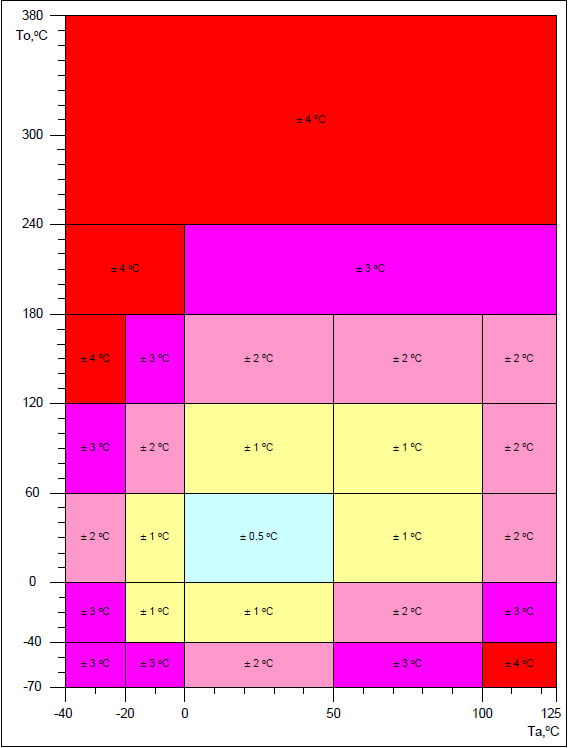
\includegraphics[width=0.5\linewidth]{res/sensor_accuracy.png}
  \caption{Temperature accuracy of the MLX90614ESF}
  \label{fig:accuracy}
\end{figure}

Figure \ref{fig:sensor} shows the wiring diagram of the sensor.
A voltage divider is used to provide a supply voltage of 3.3 V.
While the MLX90614ESF supports both pulse width modulation (PWM) and inter-integrated circuit (I2C) as its output, the latter is chosen as it provides a higher accuracy \cite{se7}.
C1 is for decoupling purposes.

\begin{figure}[H]
  \centering
  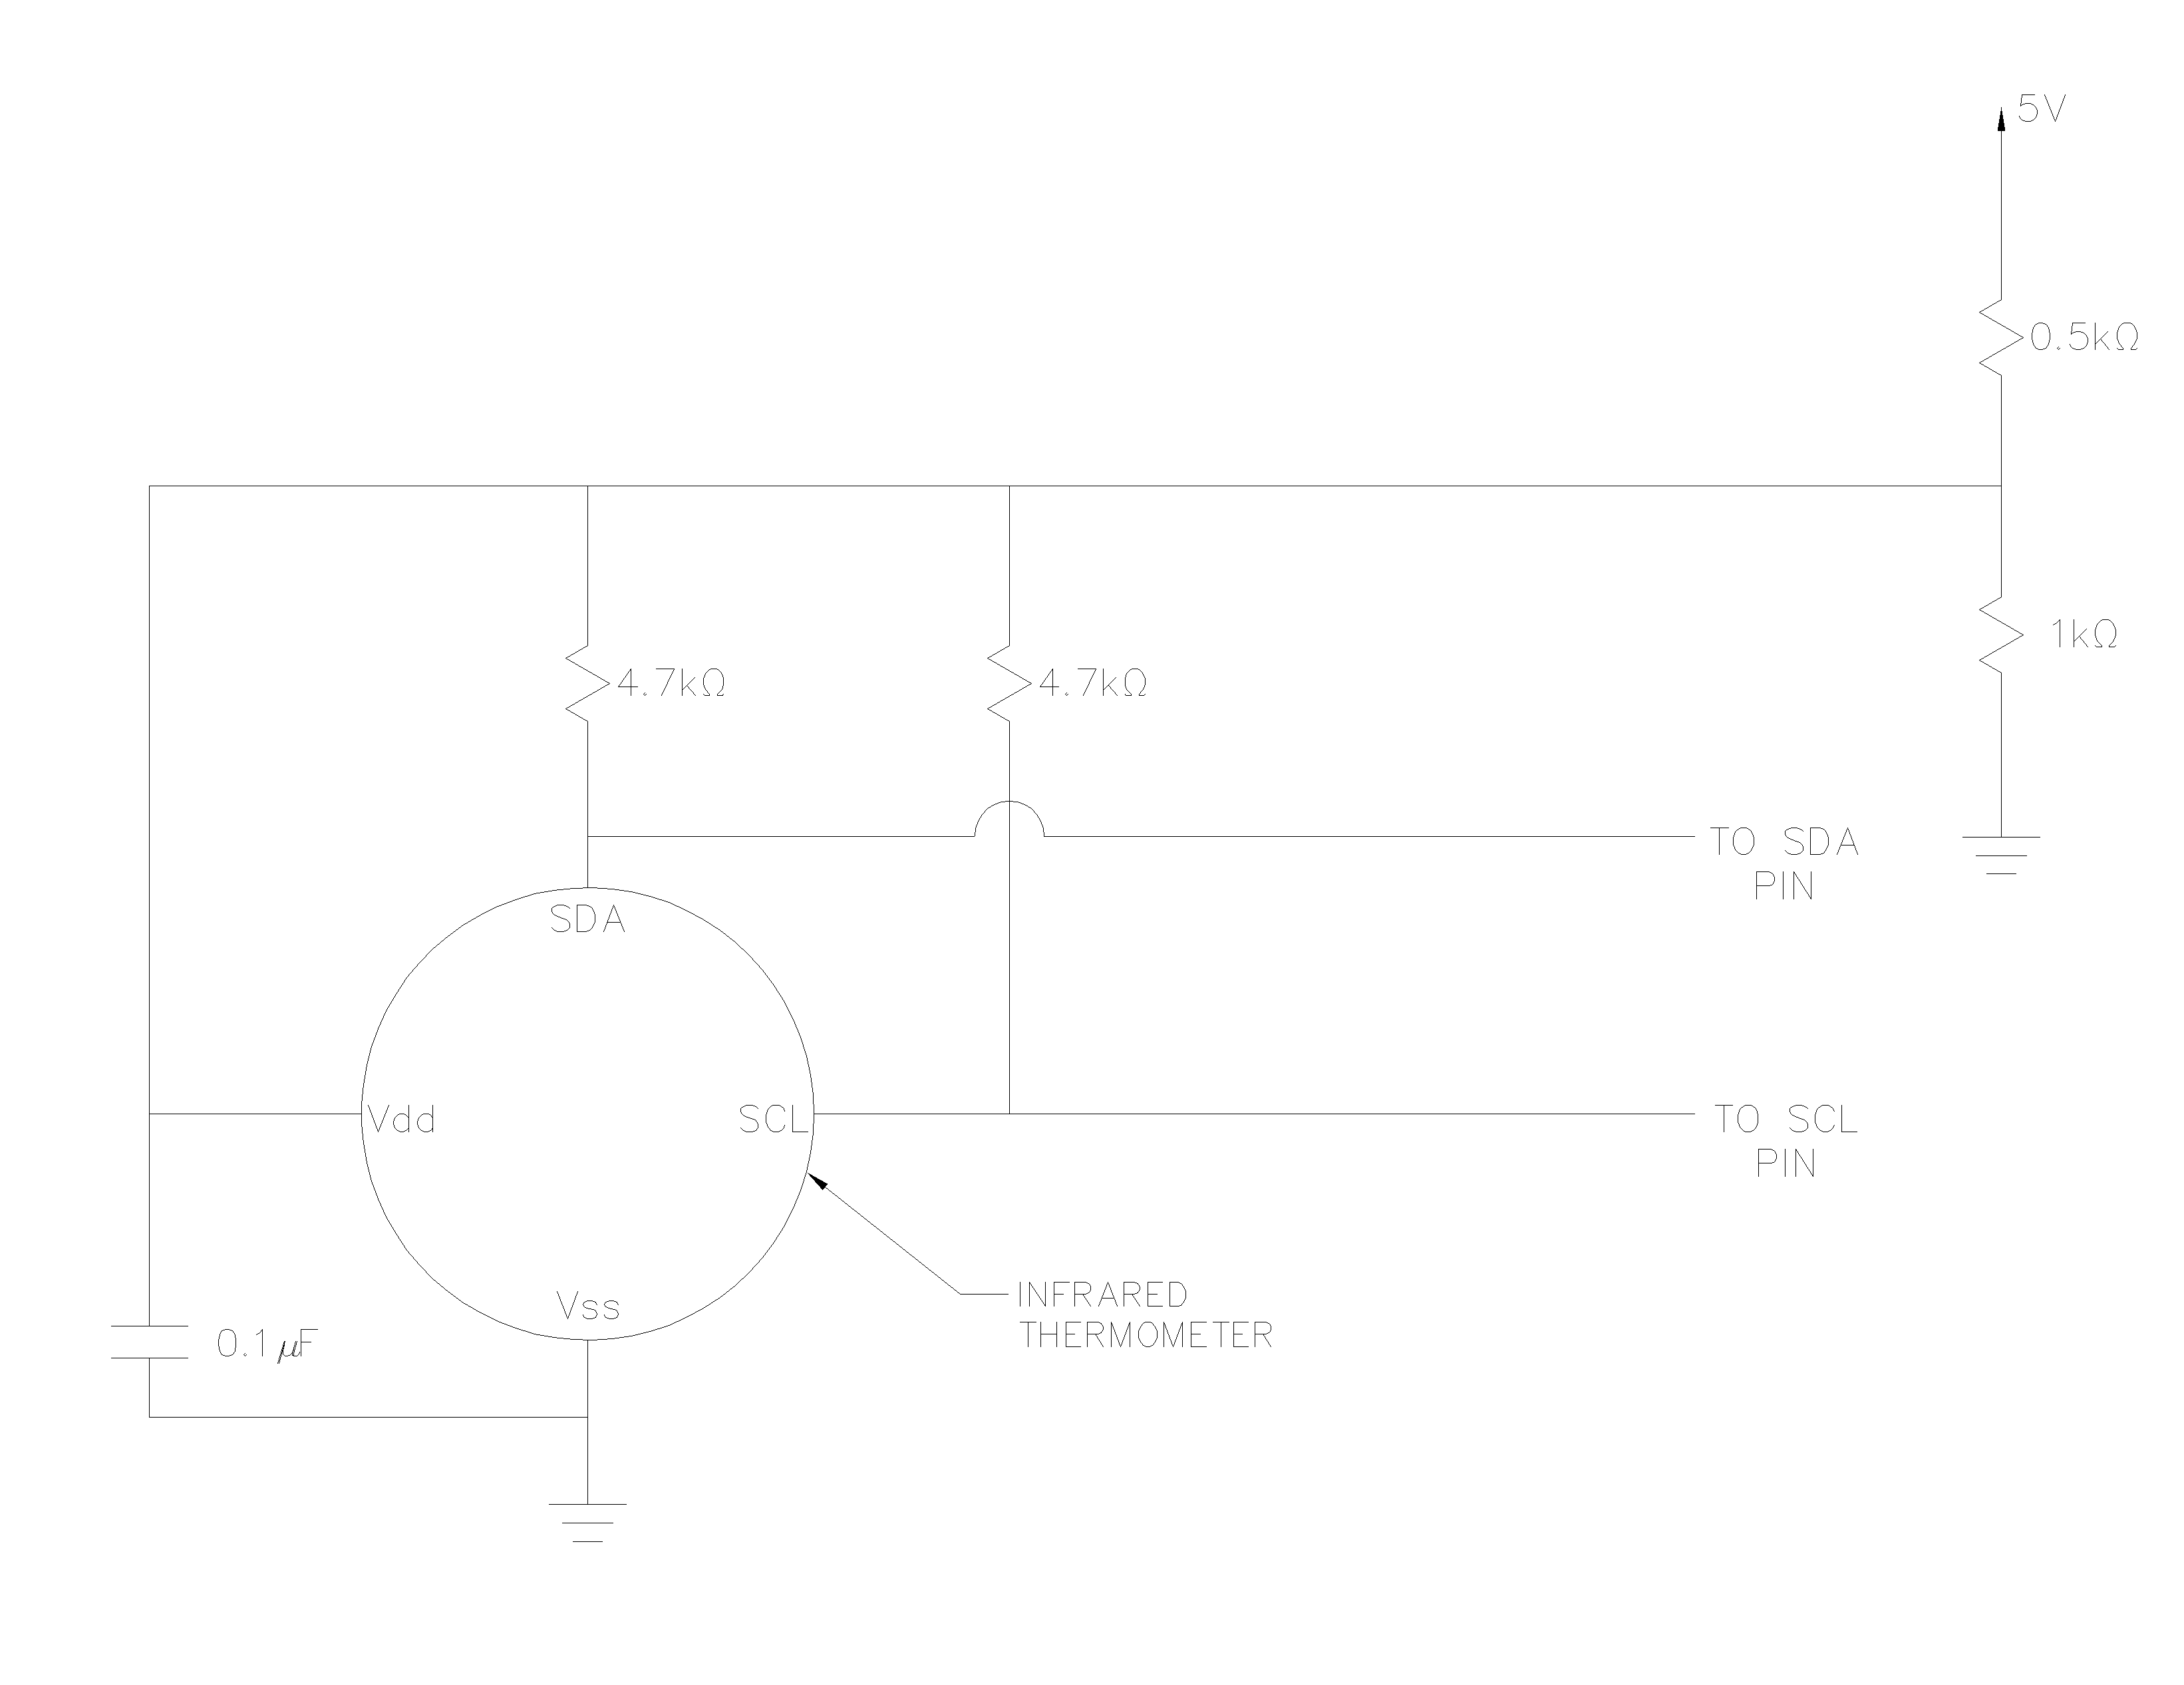
\includegraphics[width=0.6\linewidth]{res/sensor.png}
  \caption{MLX90614ESF wiring diagram}
  \label{fig:sensor}
\end{figure}

\subsection{Electrical Subsystem}

This section discusses the various components that go into the electrical design of the device.
For the purpose of this report, the components that are a part of the electrical subsystem are the motors, and the systems that control the functionality of said motors.

\subsubsection{Motors}

The following subsections outline the motor design aspect of the electrical subsystem.

\subsubsubsection{Evaluation Criteria}

\noindent
Table \ref{table:motor criteria} shows the criteria by which the motor designs are evaluated.

\begin{table}[H]
\begin{tabularx}{\textwidth}{X  r}

\hline

Criterion & Weight \\

\hline

Cost & 30 \\
Availability  & 20 \\
Precision & 20 \\
Ease of programming & 25 \\
Required number of inputs & 5 \\

\hline

\end{tabularx}
\caption{Motor design criteria}
\label{table:motor criteria}
\end{table}

The cost of the system is the highest weighted factor as the project must be kept within the budget.
The availability of the components in each system is an important factor due to the limited time available in implementing the design.
Likewise, the precision of the device is also a concern as the motors need to accurately and consistently obtain the same results for prolonged use of the device.
The ease of programming with the other subsystems is another important factor due to the limited time of the project.
Lastly, the number of inputs pins needs to accommodate the chosen microcontroller’s available I/O pins.
It has been assigned the lowest weight, however, as with a proper choice of microcontroller it should not be a major concern.

\subsubsubsection{Overview of Candidate Designs}

\noindent
There are two types of motors considered for use in this project: stepper and servo.

The first solution is the stepper motor.
Stepper motors rotate a set degree every time the signal is applied, allowing for easy replication \cite{se8}.
However, since there are set steps, the angle is only rotatable by a multiple of the set step, but this is not a problem as the steps sizes are small enough such that a high level of precision is maintained.
Overall, for the purposes of the project, the angles are achievable by all commercial stepper motors.

There are multiple configurations for the wiring that are achievable with stepper motors, but every solution would require four outputs from the microprocessor.
This allows for easily identifiable wiring no matter what configuration is used.
There is example code for this type of motor online, as well as an Arduino library, with the only adjustments to the example code being the configured revolutions per minute (RPM), direction and number of steps, a relatively easy task.

The other option is to use servo motors.
Servo motors are small in size and very energy efficient.
They generally consist of a small DC motor, potentiometer  and a dedicated control circuit, which uses PWM.
Servo motors can turn 90 \degree in either direction for a total of 180 \degree of movement and have a very precise control of position \cite{se9}.
Moreover, servo motors provide feedback to the user. Similar to stepper motors, example code and an Arduino library exists for servo motors. 

\subsubsubsection{Evaluation of Designs}

\noindent
In terms of cost and availability, stepper motors are readily available via Rigidware and thus have no shipping wait times.
These motors including their respective power supplies cost \$ 40.

Stepper motors are precise enough for the purposes of The Copper Chef and therefore receive a score of 8 for the precision criterion.
Moreover, since example code and an Arduino library are so readily available and easily adjustable, the stepper motors have achieved a score of 10 for the ease of programming criterion.
This is because stepper motors are simpler to drive in general as moving them to a specific position requires only the number of steps at the frequency required.
Stepper motors require a total of 2 control pins from the microcontroller, 1 for speed control and 1 for direction.
The motors also require 2 additional power wires for power and ground respectively.

Alternatively, servo motors that meet similar specifications cost approximately \$ 35 each for a total of \$ 105 and would require an additional 5 days shipping.
Servo motors, however, are more precise as their counterparts and so are assigned a complete score of 10 for the precision criterion.

Similar to stepper motors, there exists an Arduino library and example code for servo motors.
However, making adjustments to the existing code to meet the specifications of The Copper Chef is more complicated as stepper motors require position encoders to determine their current position and more complex code to drive the motor to the new desired position.
For this reason, stepper motors are assigned a score of 7 for ease of programming.
Lastly, a servo motor requires two power connections.
The overall circuit also contains 1 control signal from the microcontroller as well as a connection for the closed loop feedback from a position encoder.
This results in a total of 2 pins required from the microcontroller similar to the stepper motor.
Table \ref{table:motor matrix} below summarizes these discussions in a weighted decision matrix.

\begin{table}[H]
\begin{tabularx}{\textwidth}{m{5cm} r Z Z Z Z Z Z}
  \hline
  & & \multicolumn{3}{c}{Stepper Motors} & \multicolumn{3}{c}{Servo Motors} \\ 
  Criterion & Weight & S & N & W & S & N & W \\

  \hline

  Cost & 30 & 0.025 & 1 & 30 & 0.01 & 0.4 & 12 \\
  Availability & 20 & 1 & 1 & 20 & 0.2 & 0.2 & 4 \\
  Precision & 20 & 8 & 0.8 & 16 & 10 & 1 & 20 \\
  Ease of programming & 25 & 10 & 1 & 25 & 7 & 0.7 & 17.5 \\
  Number of pins & 5 & 0.5 & 1 & 5 & 0.5 & 1 & 5 \\

  \hline

  \multicolumn{5}{r}{96} & \multicolumn{3}{r}{58.5} \\

  \hline

\end{tabularx}
\caption{Computational decision matrix for the motor design}
\label{table:motor matrix}
\end{table}

From the matrix above, stepper motors are a better choice than servo motors by 40\%.

\subsubsubsection{Final Design}

\noindent
From Table \ref{table:motor matrix}, it is concluded that stepper motors are the superior option and are therefore used in the Copper Chef.
In general, servo motors cost more but are more precise than stepper motors and provide feedback to the user.
However, a lot of these features are unnecessary and stepper motors are sufficient for the scope of this project.

As part of a \$ 40 rigidware kit, three VEXTA PK266-02A by Oriental Motor \cite{se11} and ProboStepVX drivers \cite{se12} were purchased.
These motors are 2-phase, unipolar stepper motors.
This means the phases are always energized in the same way \cite{se13}.
They have a 1.8 degree step, which translates to a 200 step/revolution motor \cite{se13}.
There was also a hub-board included in the kit that combines the inputs from the stepper motor drivers and connects them to the microcontroller through two pins.

The figure below shows the wiring for the driver.
The wiring to the motor can be seen as being configured for unipolar use.
The drivers take 12 VDC from the power supply.

\subsubsection{Power Distribution}

The power distribution subsystem should be designed to transform and deliver power from a conventional North American receptacle to the power required by each component.
The power distribution system needs to be closely coordinated with other systems to provide adequate power.
The different power distribution options are directly affected by the components used in the other subsystems.
The power received from the source is transformed, converted if necessary and distributed to the different subsystems to ensure proper functionality.

\subsubsubsection{Evaluation Criteria}

\noindent
Table \ref{table:power criteria} shows the criteria by which the power distribution designs are evaluated.

\begin{table}[H]
\begin{tabularx}{\textwidth}{X  r}

\hline

Criterion & Weight \\

\hline

Cost & 30 \\
Availability & 25 \\
Ease of integration with other subsystems & 20 \\
Power consumption & 15 \\
Number of converters/transformers & 10 \\

\hline

\end{tabularx}
\caption{Power distribution system design criteria}
\label{table:power criteria}
\end{table}

For similar reasons, cost and availability of the power distribution subsection have similar weightings to that of the motors subsection.
However, since the presence of the power distribution system is necessary to do work and test the other subsystems, the power distribution availability has a slightly heavier weighting.

After cost and availability, ease of integration of with other subsystems is the most important factor when designing the power distribution system.
Since every subsystem would require a different source voltage (low voltages for microcontroller, interface components and controls, medium voltage for motor power), a complex distribution system would not only be more time consuming but also lead to more potential faults.

The overall power consumption of the device determines the potential safety concerns and the amount of electrical protection required.
It also determines the overall efficiency of the device such that between multiple distribution systems with similar functional capabilities, the one with less power draw is generally preferred.
Since one of the specifications is to use a generic power receptacle as the source powering the entire device, every design candidate for the distribution system is limited to a similar max power consumption which causes this evaluation criteria to be lower in weighting than those described above.

Transformers and converters are the main components of the distribution system and determine the size of the overall system.
However, since the device is a kitchen appliance, the scale of the power distribution is small and varying number of transformers and converters would not have a significant impact on the project.

\subsubsubsection{Overview of Candidate Designs}

\noindent
The two design candidates that can be considered for the power distribution system are AC or DC power.

With an AC distribution system, AC motors can be fed directly from building power by their respective drivers.
An AC/DC converter is then required to convert and drop the voltage to supply the microcontroller.
Any controls, signals or low voltage components are supplied by the microcontroller outputs.
See Figure \ref{fig:ac} for a high level wiring diagram.

\begin{figure}[H]
  \centering
  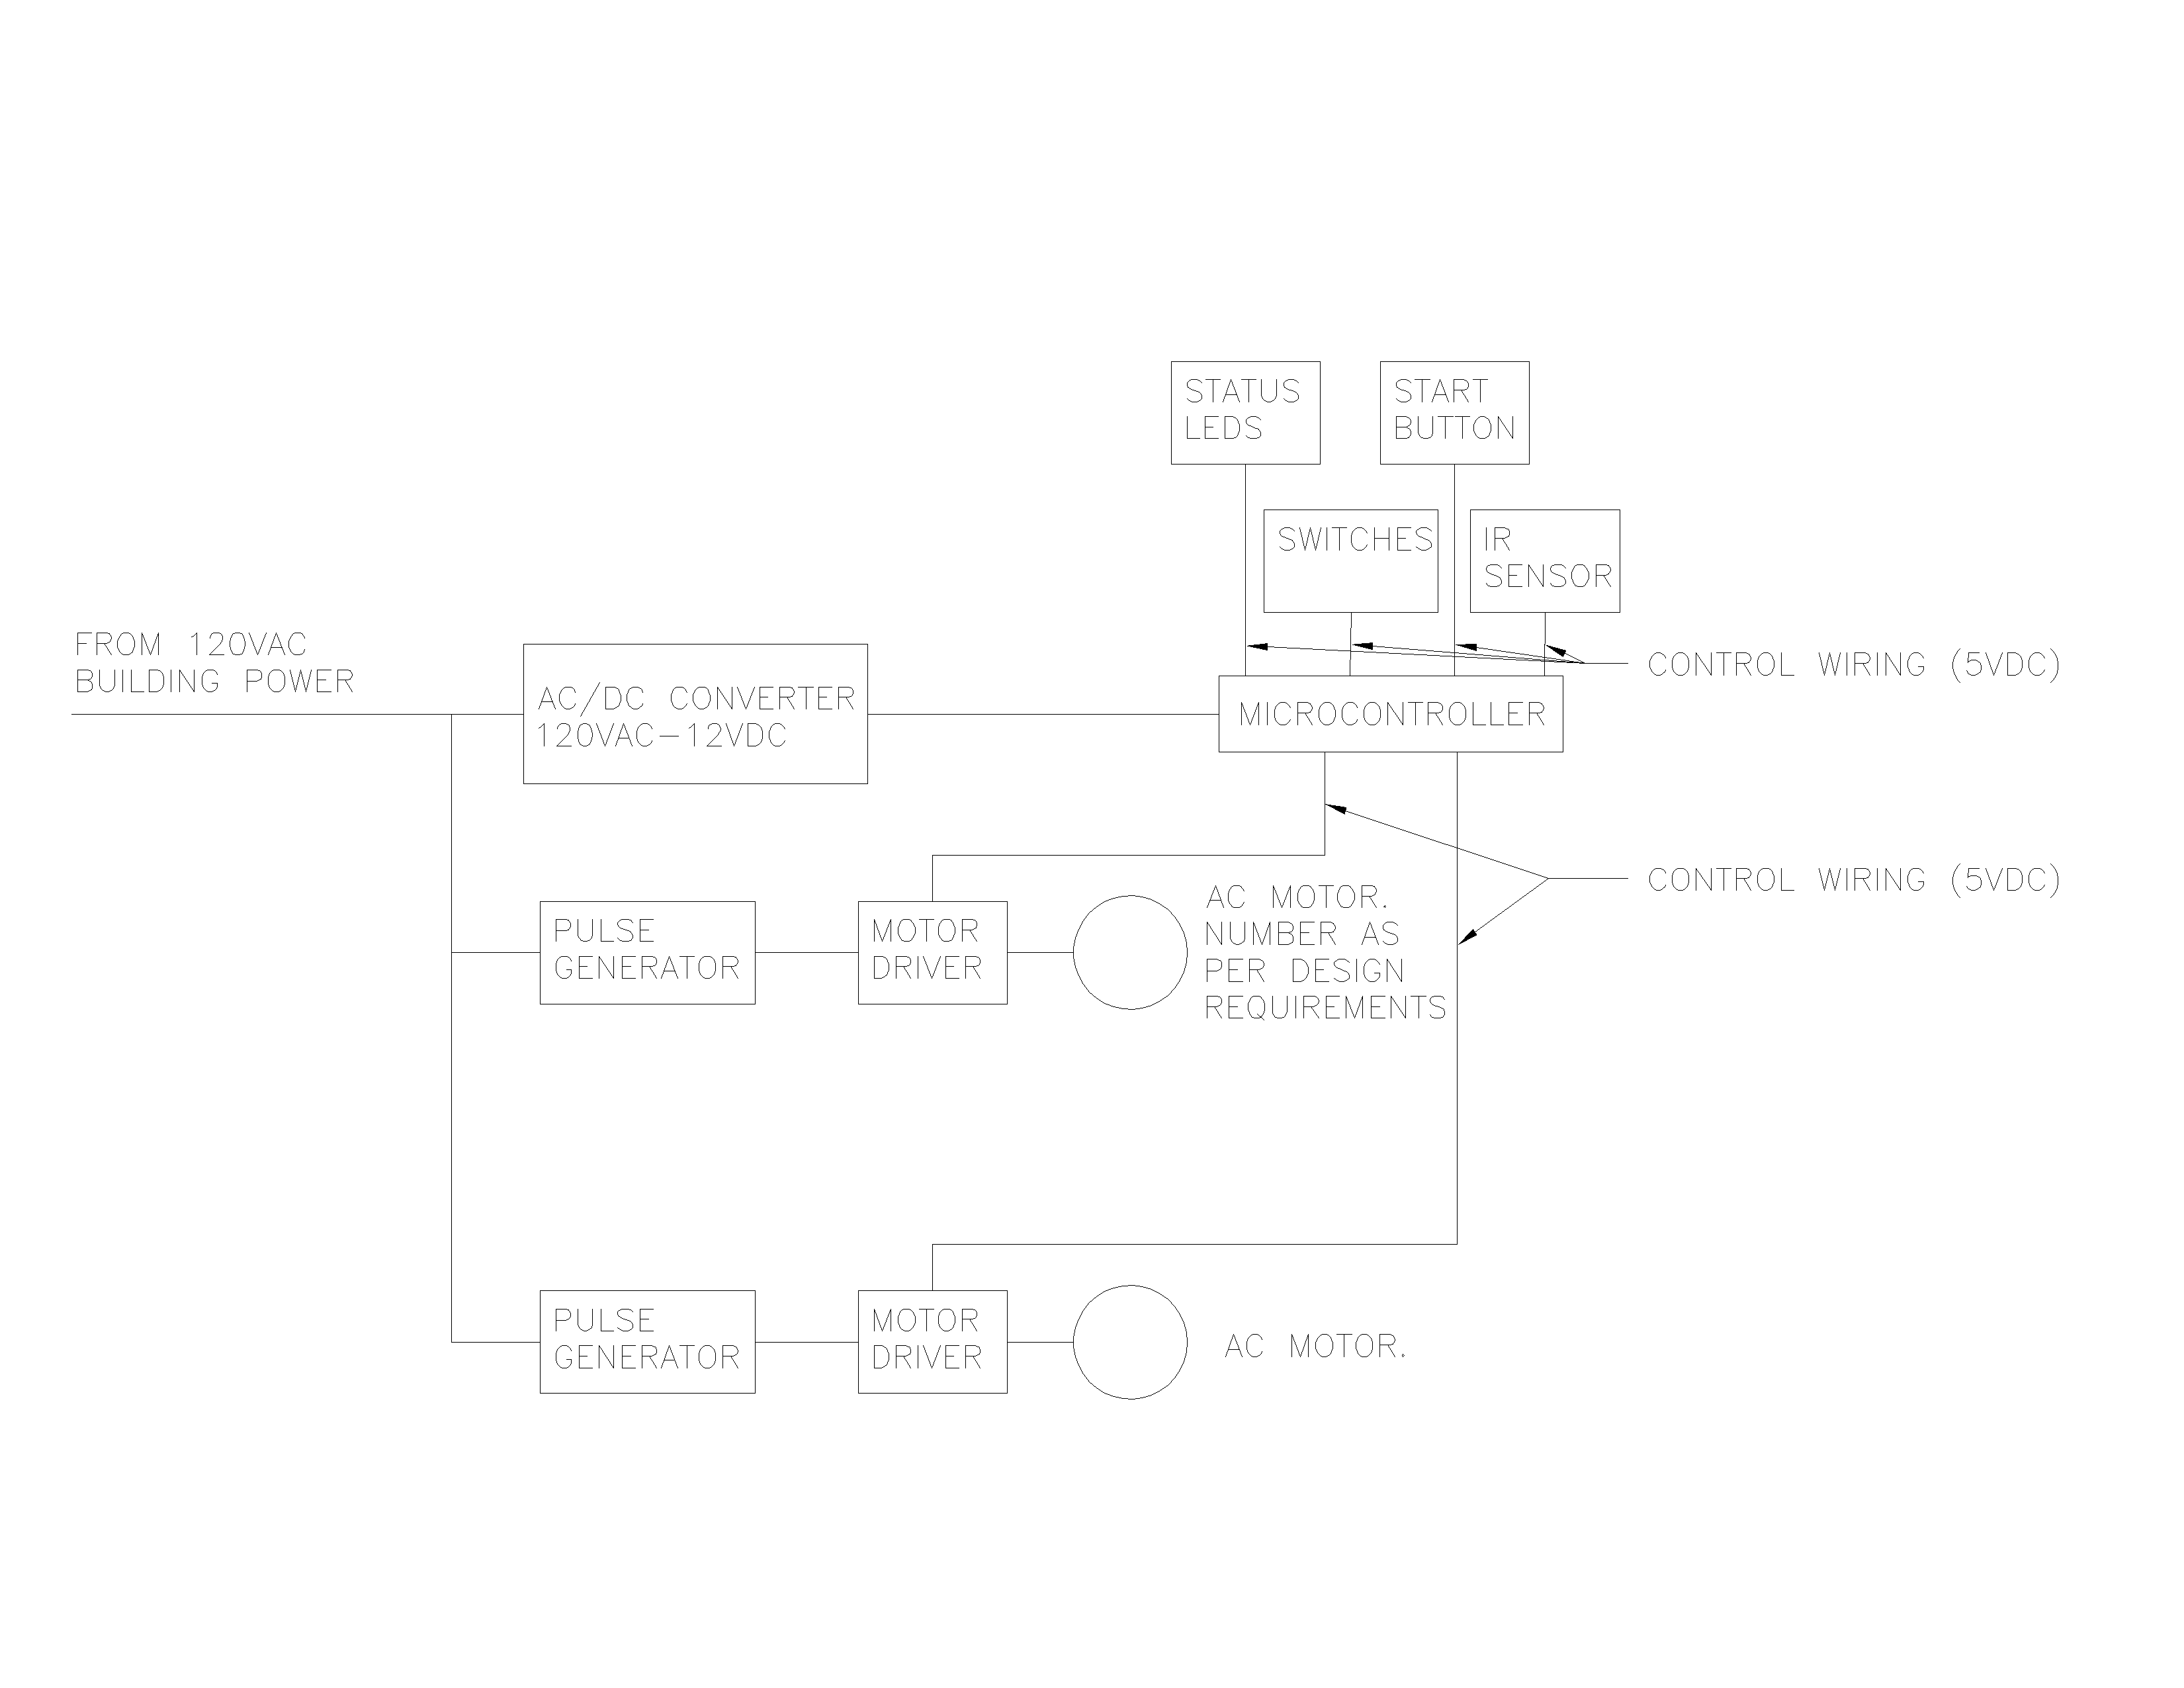
\includegraphics[width=0.6\linewidth]{res/ac.png}
  \caption{AC motor design}
  \label{fig:ac}
\end{figure}
 
With a DC distribution system and thus DC motors, an initial power converter is required to convert and step down the voltage to power the motors.
A transformer is then needed to further step down the voltage for the microcontroller which in turn supplies any low voltage and signal outputs similar to the AC design.
See Figure \ref{fig:dc} for a high level wiring diagram.

\begin{figure}[H]
  \centering
  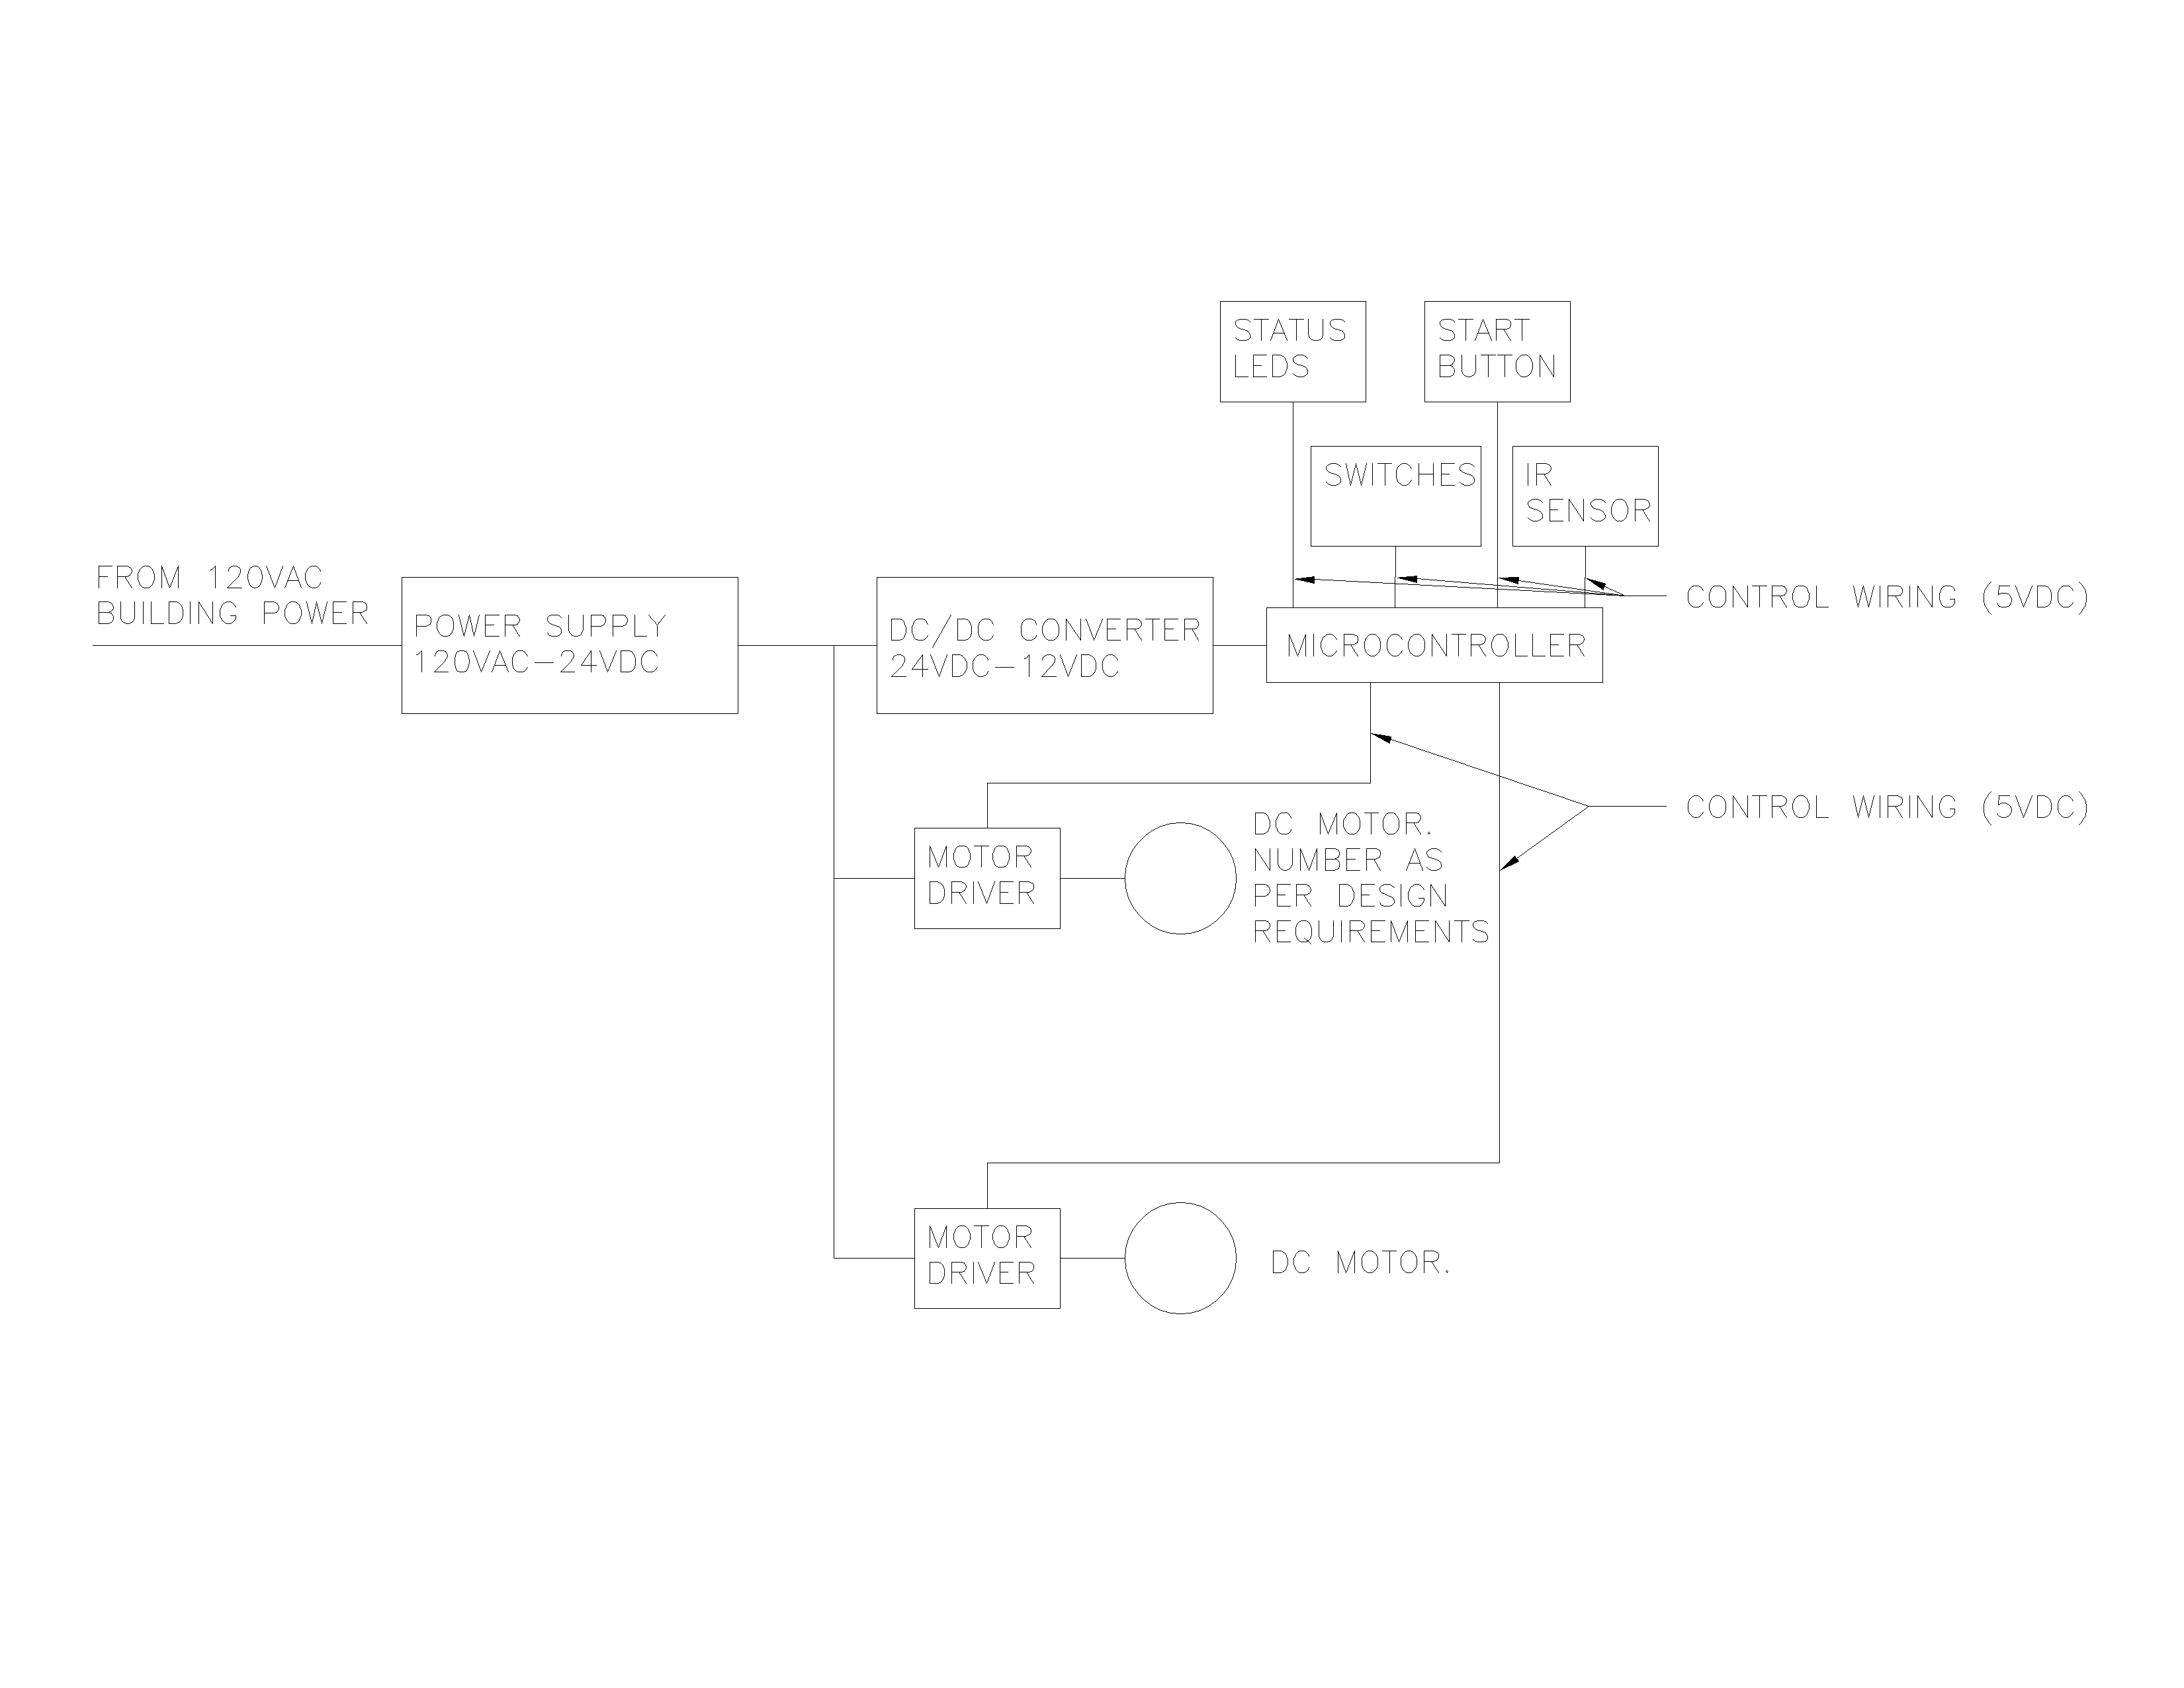
\includegraphics[width=0.6\linewidth]{res/dc.png}
  \caption{DC motor design}
  \label{fig:dc}
\end{figure}

\subsubsubsection{Evaluation of Designs}

\noindent
When evaluating the options by availability, DC motors, power supplies and drivers are readily available from Rigidware while AC motors require purchasing from an online source and would require a 7 business day waiting time.
The cost for the DC power supply, 3 DC motors and all necessary components were \$ 40 from Rigidware.
The cheapest available AC components of similar performance specs found online were \$ 25 for the power supply and \$ 35 for each motor.
Although the DC system does require an additional transformer, the costs saved from the motor components significantly outweighs these and any further additional costs.
A summary for the cost comparison can be seen in Table \ref{table:power costs} below.
The DC system costs approximately half of the AC system and the major components are more readily available.

\begin{table}[H]
\begin{tabularx}{\textwidth}{X Z Z Z Z Z}

  \hline

  & Motors with drivers & Power Supply & Additional transformers & Misc. items & Total \\

  \hline

  AC system & 35 each & 25 & 0 & 10 & 140 \\
  DC system & 40 & 0 & 20 & 10 & 70 \\

  \hline

\end{tabularx}
\caption{Costs of power distribution candidates}
\label{table:power costs}
\end{table}

AC motors benefit by being able to give a larger torque than DC motors of the same power consumption.
This allows for the usage of motors with a lower power consumption than in the DC system which in turn allows for less losses throughout the AC system and more overall efficiency \cite{power_efficiency}.
Due to the efficiency of AC motors, it is assigned a score of 4 out of 10, and DC motors are assigned a score of 10 out of 10.

When comparing number of transformers/converters, the DC system requires the voltage to be stepped down twice, once for the motors and once again for the microcontroller and low voltage components, whereas with the AC system, motors can be purchased which are compatible with the AC building power and as such only a single converter is required for the microcontroller.
This difference allows for a smaller overall potential AC system by one main component. 

After evaluating both systems, it can be seen from the wiring diagrams that they are both fairly similar in terms of complexity with the exception of the additional DC transformer.
All low voltage components fed from the microcontroller remains consistent between designs and thus the only significant difference would be how the motors and microcontroller are fed.
Since AC motor speeds are controlled by varying the frequency armature current, additional pulse generators are required for the AC system.
This however does not lead to a significant increase in complexity as most motor drivers are usually equipped with the necessary pulse generator.
If we assign the AC system with a perfect score for ease of integration, the DC system would then have a relative score of 8 out of 10 for the additional connection and potential mode of failure at the DC step down transformer.

\begin{table}[H]
\begin{tabularx}{\textwidth}{m{5cm} r Z Z Z Z Z Z}
  \hline
  & & \multicolumn{3}{c}{AC system} & \multicolumn{3}{c}{DC system} \\ 
  Criterion & Weight & S & N & W & S & N & W \\

  \hline

  Cost & 30 & 0.007 & 0.5 & 15 & 0.014 & 1 & 30 \\
  Availability & 25 & 0.143 & 3.6 & 1 & 1 & 25 \\
  Ease of integration & 20 & 10 & 1 & 20 & 8 & 0.8 & 16 \\
  Power consumption & 15 & 10 & 1 & 15 & 4 & 0.4 & 6 \\
  Number of transformers/converters & 10 & 1 & 1 & 10 & 0.5 & 0.5 & 5 \\

  \hline

  \multicolumn{5}{r}{63.6} & \multicolumn{3}{r}{82} \\

  \hline

\end{tabularx}
\caption{Computational decision matrix for the power distribution system design}
\label{table:power matrix}
\end{table}

Based on the table above, the DC power distribution system is 22.4 \% better than the AC distribution system.

\subsubsubsection{Final Design}

\noindent
A Potrans FS-15024-1M \cite{se14} power supply purchased with the Rigidware kit is used for the power distribution network.
The FS-15024-1M can supply up to 24 VDC at 6.5 A.
The wiring is as shown in Figure \ref{fig:dc}.
A DROK DC-DC Buck Converter 24v, 12v3a max \cite{se15} was purchased for \$ 15 to step-down the voltage to 12 V.
The microcontroller then supplies the rest of the system with 5 V.

\subsection{Interface Subsystem}

This section outlines the design of the interface that allows the user to communicate with the device, and for the device to communicate with the user.

\subsubsection{Evaluation Criteria}

Before cooking begins, the user must be able to select the doneness level to which they want their steak to be cooked from 5 different options.
The Copper Chef must also be able to communicate to the user whether the pan is too hot, too cold, or the correct temperature, and whether the steak has finished cooking.

Table \ref{table:interface criteria} shows the criteria by which the interfaces are evaluated.

\begin{table}[H]
\begin{tabularx}{\textwidth}{X  r}

\hline

Criterion & Weight \\

\hline

Electrical design cost & 25 \\
Software design cost & 25 \\
Usability & 50 \\

\hline

\end{tabularx}
\caption{Interface design criteria}
\label{table:interface criteria}
\end{table}

The overall design cost is equally weighted compared to usability.
It is important that the Copper Chef is intuitive and convenient to be used, but equally important that the design is not too complicated and difficult to implement so that more resources can be allocated to fulfilling essential specifications of the Copper Chef.
Doneness selection is a non-essential specification, so resources should not be spent on implementing an unnecessarily complex interface subsystem unless it offers a significant benefit in terms of usability.

\subsubsection{Overview of Candidate Designs}

An Android application, buttons, and a five-position switch are being considered for the user input system.

The android smartphone app allows users to communicate with The Copper Chef over Bluetooth.
The button- or switch-based designs can both be implemented with direct connections to the inputs of The Copper Chef’s microcontroller.
The app allows The Copper Chef to communicate information back to users through software using only the cell phone, whereas implementing hardware-based interface designs such as the button- or switch-based designs require the manual implementation of output signals.
At least one three-coloured LED and one alarm need to be included in the design of The Copper Chef.

\subsubsection{Evaluation of Designs}

The electrical design cost is measured by the hours it will take to implement the electrical design.
The Android application requires only a Bluetooth transceiver connected to the microcontroller, so it is relatively simple to implement.
It is estimated that it will take 1 hour, and is given a score of 1/1 = 1.
The button- and switch-based designs require the manual implementation of communication software, and it is estimated that they will take 2 hours to implement.
They each receive a score of 1/2 = 0:5.

The software design cost is measured by the hours it will take to implement the software design.
The Android application requires much more time to implement than the simple integrations required for the button- and switch-based designs.
It is estimated that the button- and switch-based designs will take approximately 2 hours to implement, while the application will take 16, resulting in scores of 1/2 = 0.5 and 1/16 = 0.0625.

Tying a piece of the functionality of The Copper Chef to an external device over which there is no control does result in reduced usability, but Android phones are prevalent, and their usage is generally well-understood.
Physical buttons on the device eliminate the need for external hardware, but they fail to persist the input parameters; if they are not received by the microcontroller when they are entered, they are simply lost.
The switch-based design solves this problem, and has the additional benefit of visibly indicating the current configuration of the system to anybody who may be looking at the device.
The usability scores received by the application, button-based, and switch-based designs are therefore assigned as 0.7, 0.6, and 0.8, respectively.

Table \ref{table:interface matrix} is the computational decision matrix for the interface system.

\begin{table}[H]
\begin{tabularx}{\textwidth}{m{5cm} r Z Z Z Z Z Z Z Z Z}
  \hline

  & & \multicolumn{3}{c}{Application} & \multicolumn{3}{c}{Buttons} & \multicolumn{3}{c}{Switch} \\
  Criterion & Weight & S & N & W & S & N & W & S & N & W \\

  \hline

  Electrical design cost & 25 & 100 & 1 & 25 & 50 & 0.5 & 12.5 & 50 & 0.5 & 12.5 \\
  Software design cost & 25 & 6.25 & 0.125 & 3.1 & 50 & 1 & 25 & 50 & 1 & 25 \\
  Usability & 50 & 70 & 0.875 & 43.8 & 60 & 0.75 & 37.5 & 80 & 1 & 50 \\

  \hline

  & & & & 71.9 & & & 76 & & & 87.5 \\

  \hline
\end{tabularx}
\caption{Computational decision matrix for the interface subsystem}
\label{table:interface matrix}
\end{table}

The switch-based solution is 15 \% better than the button-based design, and 22 \% better than
the application solution.

\subsubsection{Final Design}

The switch-based solution is chosen for the final design of The Copper Chef.
A 5-position switch is used to allow the user to select the level of doneness they would like, and three LEDs are used to communicate information about the heat of the pan.

The switch chosen is the SLS151RA Slide Switch SP5T.
It is a 5-position switch with 6 pins.
Each switch position connects two adjacent pins together.
For example, if the pins are numbered 1-6, placing the switch in the far left position connects pin 1 to pin 2.
Therefore, the switch is wired as seen below in Figure \ref{fig:switch}.

\begin{figure}[H]
  \centering
  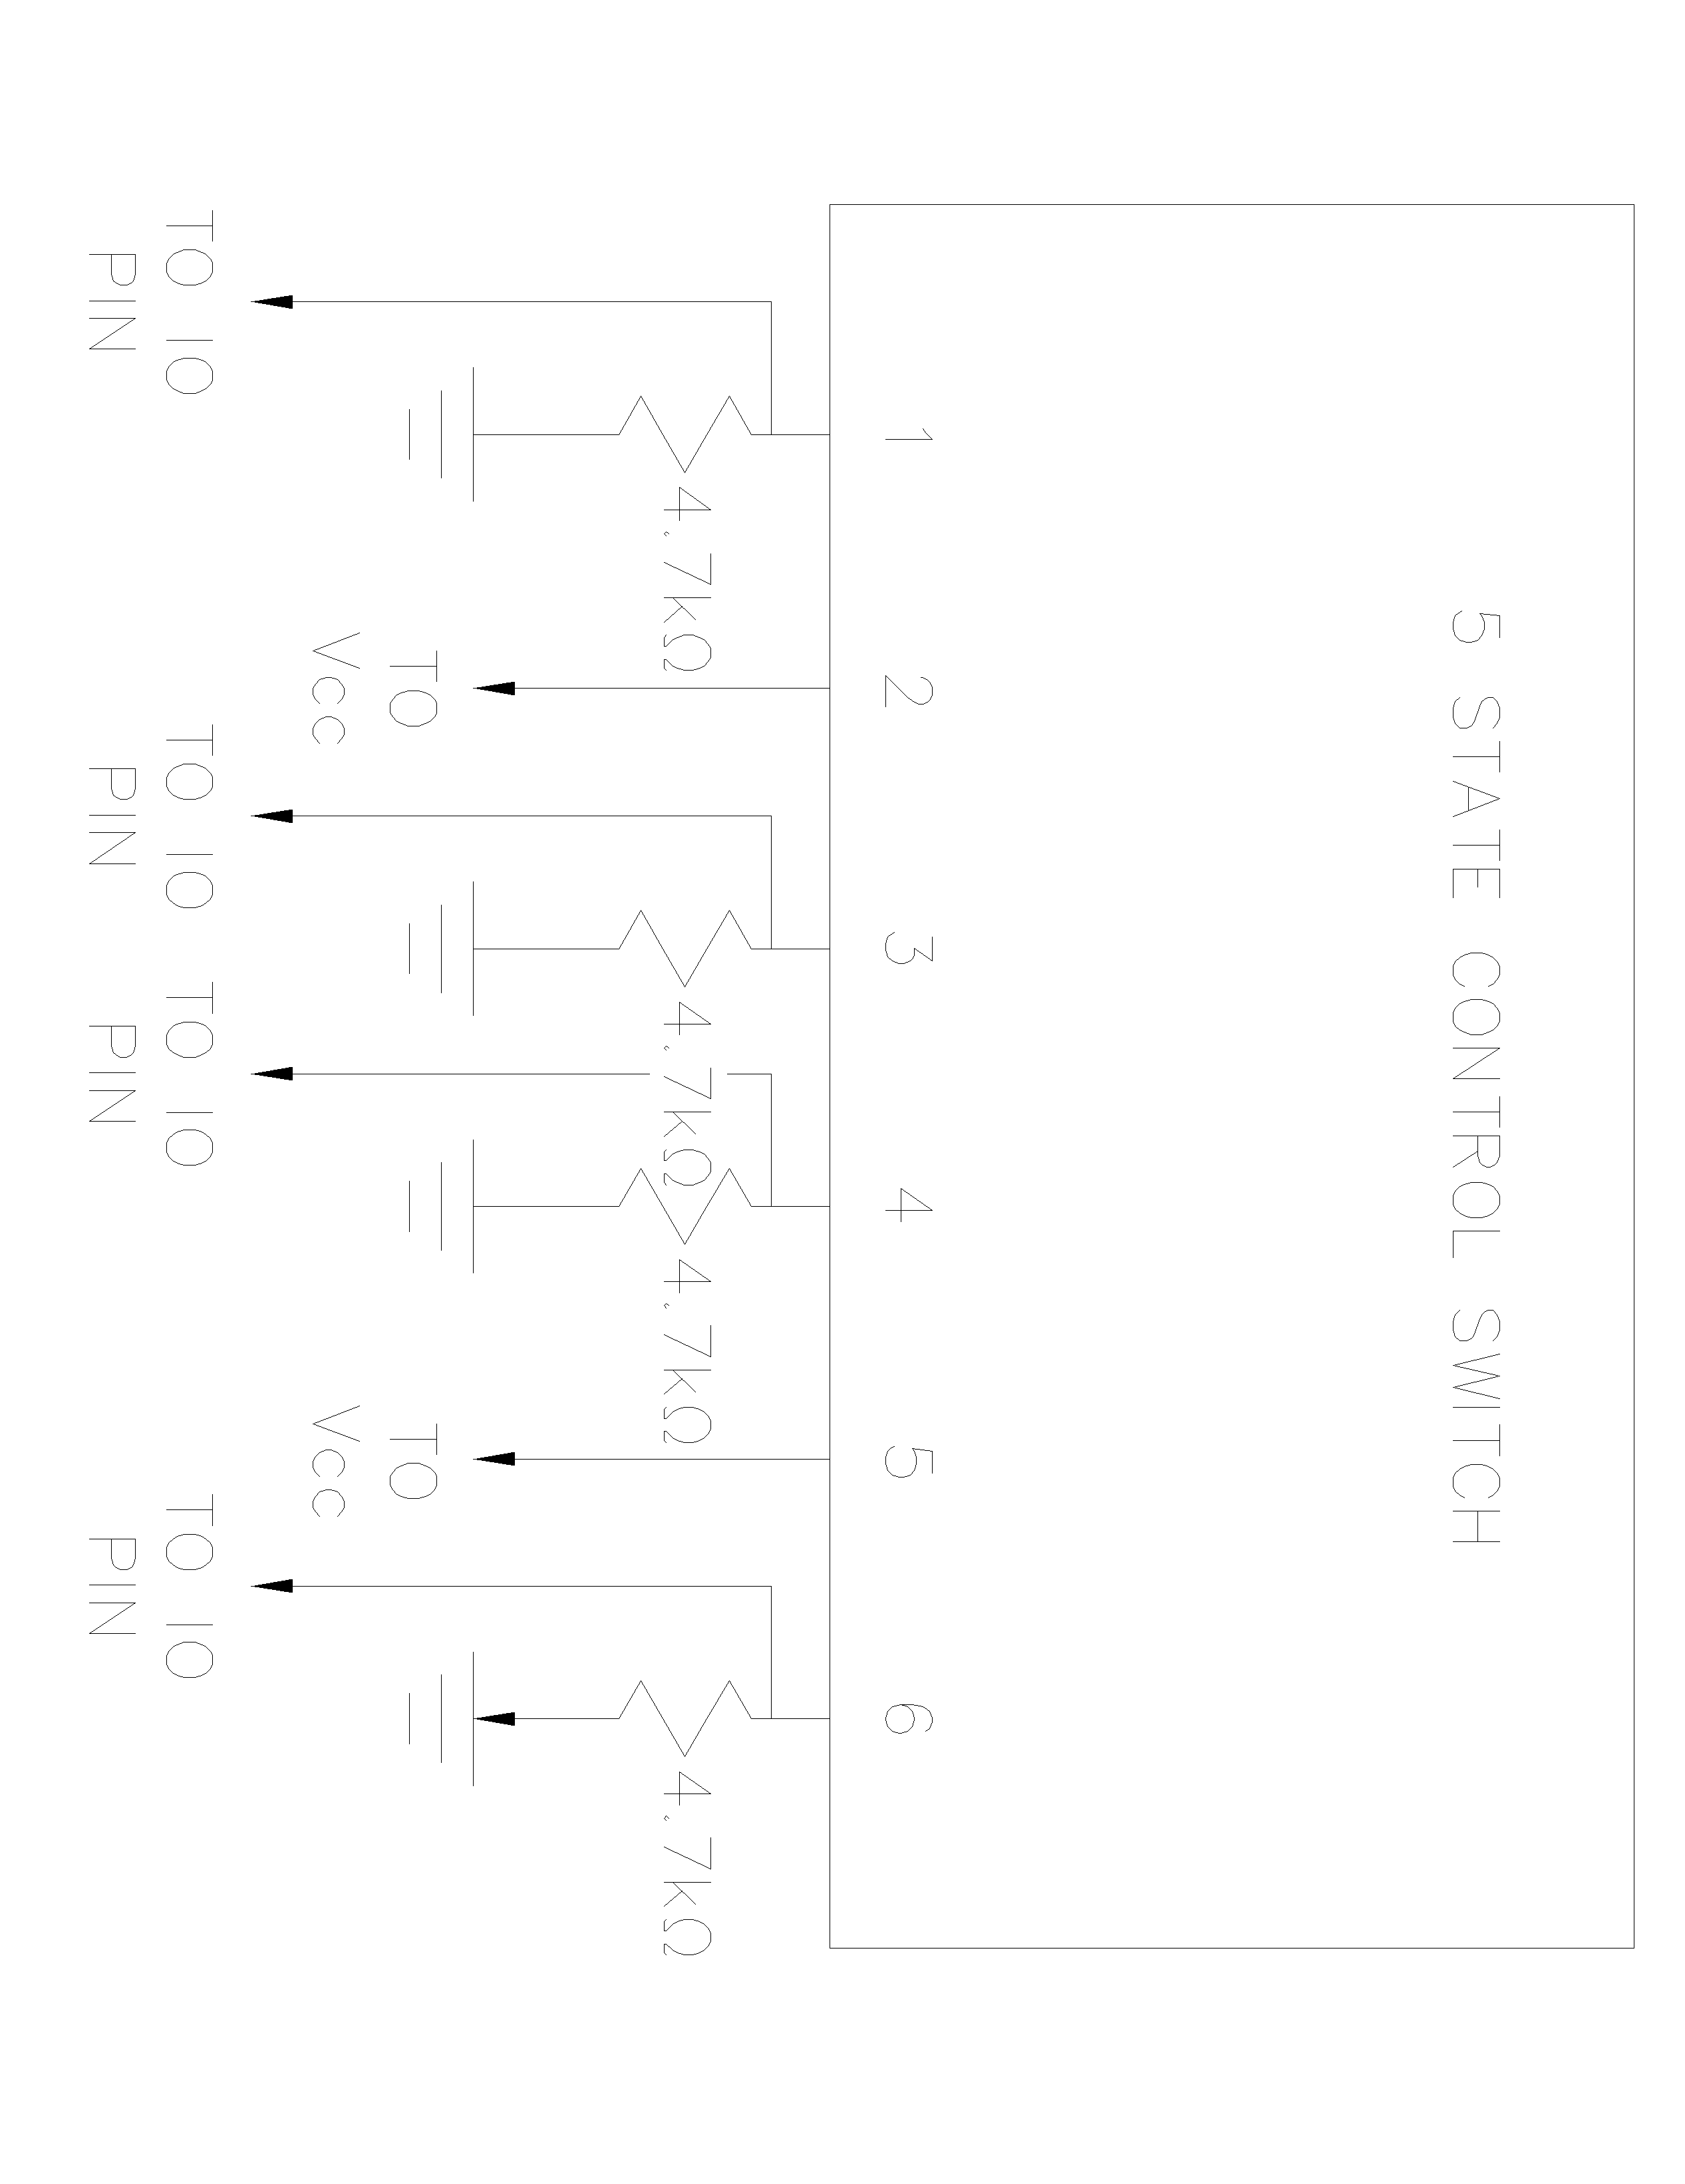
\includegraphics[width=0.4\linewidth, angle=90]{res/switch.png}
  \caption{Switch wiring diagram}
  \label{fig:switch}
\end{figure}

Pulldown resistors are used to ensure any pin not connected to Vcc stays low. Additionally, pins 1, 3, 4, and 6 are connected to input pins on the microcontroller.  Pins 2 and 5 are not used as inputs to the microcontroller because they are always high. It can be seen that 5 states can be derived depending on each of the states of the input pins. Note that Position 1-2 in Table \ref{table:switch positions} refers to the switch position that connects pins 1 and 2 together.

\begin{table}[H]
\begin{tabularx}{\textwidth}{X Z Z Z Z}

  \hline

  & Pin 1 & Pin 3 & Pin 4 & Pin 6 \\

  \hline

  Position 1-2 & 1 & 0 & 0 & 0 \\
  Position 2-3 & 0 & 1 & 0 & 0 \\
  Position 3-4 & 0 & 0 & 0 & 0 \\
  Position 4-5 & 0 & 0 & 1 & 0 \\
  Position 5-6 & 0 & 0 & 0 & 1 \\

  \hline

\end{tabularx}
\caption{Switch position states}
\label{table:switch positions}
\end{table}

\subsection{Software Subsystem}

This section discusses the software of The Copper Chef.

\subsubsection{Microcontroller}

This section compares the merits of three candidate components that can be used as a microcontroller in The Copper Chef.

\subsubsubsection{Evaluation Criteria}

\noindent
The first step in choosing a microcontroller is to determine a set of minimum requirements for the potential microcontroller to meet.
In terms of input and output, it can be seen that the Copper Chef requires a minimum of 4 inputs and 9 outputs, as follows:

\begin{itemize}
  \item three digital inputs for user interface switches
  \item one digital input for button to start cooking process
  \item four analog or digital outputs for LED control
  \item two analog or digital outputs to control the translational motor
  \item one analog or digital output to control the rotational motor
  \item one digital PWM output to control the speed of the motors
  \item one I2C input for the IR thermometer
\end{itemize}

Thus, any microcontroller with at least four digital inputs, seven analog or digital outputs, one digital PWM output, and one I2c input could be a suitable choice for The Copper Chef. There is no obvious benefit to exceeding this minimum requirement except to have extra I/O in case of design changes.

Table \ref{table:high_level_criteria} shows the criteria by which the microcontrollers are evaluated.

\begin{table}[H]
\begin{tabularx}{\textwidth}{X  r}

  \hline

  Criterion & Weight \\

  \hline

  Ease of interfacing & 40 \\
  Availability of documentation & 40 \\
  Group member experience & 10 \\
  Cost & 10 \\

  \hline

\end{tabularx}
\caption{Microcontroller criteria}
\label{table:microcontroller criteria}
\end{table}

Ease of interfacing refers to how suitable the device is to fulfill The Copper Chef’s logic purposes with code that is simple, short, and unobfuscated.
Ease of interfacing and availability of documentation are both weighted at 40 \%.
These are the most important criteria because they represent the difficulty of implementing the logic of The Copper Chef for a particular choice of microcontroller.
Group members experience also makes it easier to implement the logic of The Copper Chef, but this is weighted at only 10 \% because our group as a whole does not have extensive experience with any of the options.
Cost is weighted at 10 \% because no option is particularly expensive, and furthermore the cost of a microcontroller is only a small component of the overall cost of The Copper Chef.

Power consumption was also considered as a potential criterion, but was ultimately left out of the decision matrix since the power consumption of each microcontroller is very low when compared to the power consumed by the rest of the system.
Moreover, a small adapter is being used to supply the power,and this adapter can provide tens of watts, but the microcontroller only requires a few watts.

The number of bits for the processor and amount of memory included in the processor are also not included in the decision matrix, as any options should provide the minimum requirement due to the simplicity of computation needed by the Copper Chef.
 For example, there is no real advantage to using a 32-bit processor versus an 8-bit for the required computations.
Moreover, the development environment and debuggers available for various microcontrollers are also not considered and compared for the same reason.

\subsubsubsection{Overview of Candidate Designs}

\noindent
The Raspberry Pi 3 Model B, Ardino Mega 2560 R3, and TI LaunchPad MSP430FR4133 are being considered for The Copper Chef's microcontroller.

All of these options fulfill the minimum I/O and processing power requirements of The Copper Chef.
The Raspberry Pi and Arduino platforms are the ubiquitous choice to control small electronics projects.
The Raspberry Pi 3 Model B is chosen as a candidate since it is the newest model of Raspberry Pi and is most readily available.
The Arduino Mega 2560 R3 is chosen since it is readily available from RigidWare.
TI LaunchPad MSP430FR4133 LaunchPad Development Kit is chosen because it is readily available and because a group member had previous experience working with this particular model.

The Arduino and TI LaunchPad are both microcontrollers, whereas the Raspberry Pi is more accurately described as a single-board computer.
This means that Arduino and TI LaunchPad are typically used to run a single program at a time, typically performing simple, repetitive tasks involving interfacing with sensors or other devices \cite{eb1}\cite{arduino_pi}.

On the other hand, a Raspberry Pi is more like a typical desktop computer, and is therefore more versatile: it runs a linux-based operating system, can run multiple programs at once, and has features such as a graphics processing unit (GPU) \cite{arduino_pi}.

\subsubsubsection{Evaluation of Designs}

\noindent
The Arduino is assigned a score of 9 for ease of interfacing, whereas the Raspberry Pi and TI LaunchPad are assigned a scores of 6.
These scores are quite subjective, and difficult to determine due to the limited experience the design team has with each option.
Although preliminary research indicated that a microcontroller such as an Arduino or TI LaunchPad was a more suitable platform for a simple program involving interfacing with sensors and motors, it was found that it is fairly simple to interface with LEDS, switches, and buttons on all three platforms, and that software libraries can be found for all three platforms that simplify working with stepper motors \cite{eb2} \cite{eb3} \cite{eb4}.
 The main reason why Arduino is given a higher score is that it is easier to find a temperature sensor that is designed to work with an Arduino: a suitable temperature sensor was found with a prewritten library meant to make interfacing with an Arduino very easy, whereas no such sensor or library was found for the TI LaunchPad or Raspberry Pi.

The Raspberry Pi is assigned a score of 9 for availability of documentation, whereas the Arduino is assigned a 8 and the TI launchpad a 5.
Again, it is difficult to assign accurate scores for this criterion, but it is widely accepted that Arduino and Raspberry Pi have detailed documentation.
Additionally many examples of sample code can be found for both the Arduino and Raspberry Pi since they are such popular choices for electronics projects.
The TI LaunchPad is far less widespread, and it is difficult to find examples of code used for projects done using the TI LaunchPad.
Furthermore, the design teams advisor and one of the group members who has used a TI LaunchPad in the past feel that the documentation for the TI LaunchPad is particularly bad.
Ultimately, the Raspberry Pi is assigned a higher score than the Arduino because more results appear on google for Raspberry Pi than Arduino.
As of June 29, 2017, 56,300,00 results are returned on google.ca for the search query Raspberry Pi, 6,800,000 results for Arduino, and 1,100,100 for TI LaunchPad.
Clearly this is not a perfect metric for determining the quantity of code documentation and samples, but it supports the idea that the Raspberry Pi has more widespread documentation, and that the TI launchpad is particularly bad in this respect.

The TI LaunchPad is assigned a score of 7 for group member experience, whereas the Arduino and Raspberry Pi are both assigned a score of 4.
Every option is programmed using the C programming language, with which each member of the design team has some basic experience.
However, one member of the design team has a moderate amount of experience working with the TI LaunchPad specifically, whereas no design team members have any experience with the other options.
Therefore the TI LaunchPad is assigned a higher score.

The TI LaunchPad and Arduino are both assigned scores of 8 for cost, whereas the Arduino is assigned a score of 6 This is because the TI launchpad costs \$ 15, but a “booster pack” costing approximately \$ 30 is needed to interface with stepper motors \cite{eb5} \cite{ti2}.
The Arduino similarly comes to around \$ 45 total \cite{arduino2}. A raspberry pi model 3 costs the most at around \$ 60 and is therefore given the lowest score.
All of the raw values in the matrix in Table \ref{table:microcontroller matrix} below are converted into percentages.

\begin{table}[H]
\begin{tabularx}{\textwidth}{m{5cm} r Z Z Z Z Z Z Z Z Z}
  \hline

  & & \multicolumn{3}{c}{Arduino} & \multicolumn{3}{c}{Raspberry Pi} & \multicolumn{3}{c}{TI Launchpad} \\
  Criterion & Weight & S & N & W & S & N & W & S & N & W \\

  \hline

  Ease of interfacing & 40 & 9 & 1 & 40 & 6 & 0.67 & 26.8 & 6 & 0.67 & 26.8 \\
  Availability of documentation & 40 & 8 & 0.89 & 35.6 & 9 & 1 & 40 & 5 & 0.56 & 22.4 \\
  Group member experience & 10 & 4 & 0.57 & 5.7 & 4 & 0.57 & 5.7 & 7 & 1 & 10 \\
  Cost & 10 & 8 & 1 & 10 & 6 & 0.75 & 7.5 & 8 & 1 & 10 \\

  \hline

  \multicolumn{5}{r}{91.3} & \multicolumn{3}{r}{80} & \multicolumn{3}{r}{69.2} \\

  \hline

\end{tabularx}
\caption{Computational decision matrix for the microcontroller}
\label{table:microcontroller matrix}
\end{table}

The Arduino is given a final score of 91.3, whereas the Raspberry Pi is given a score of 80, and the TI Launchpad is given a score of 69.2.
Therefore, the Arduino is chosen as the best solution.

\section{Prototype Data}

Figures \ref{fig:photo1} and \ref{fig:photo2} below show the current state of the prototype. Figure \ref{fig:photo2} is of the whole fixture and Figure \ref{fig:photo1} shows the sensor and switch connections to the microcontroller. It can be seen that the mechanical aspects of the project, such as the frame and cage, are complete. The electrical subsystem, which consists of the power supply, motors, sensor and the user interface is also complete. The power supply, however, is not shown to be connected in the image. Currently the prototype can move up and down in a vertical motion using the motors and sense temperatures. Steak cooking has been tested with the cage and it was found that there was no damage to the steak’s visible appeal. The rotary function is not yet complete, and the prototype therefore does not autonomously cook steak yet.

\begin{figure}[H]
\centering
\begin{minipage}{.5\textwidth}
  \centering
  \includegraphics[width=.6\linewidth]{res/photo1.png}
  \captionof{figure}{Switch, thermometer, and microcontroller}
  \label{fig:photo1}
\end{minipage}%
\begin{minipage}{.5\textwidth}
  \centering
  \includegraphics[width=.6\linewidth]{res/photo2.png}
  \captionof{figure}{Mechanical design}
  \label{fig:photo2}
\end{minipage}
\end{figure}

\section{Discussions and Conclusions}

This section discusses and comments on the final design of The Copper Chef.

\subsection{Evaluation of Final Design}

The design proposed in the report satisfies all of the outlined essential specifications.

Once the system determines that the steak has been completed, the motors are able to remove the steak from the heat source.
Once the steak is removed from the heat source, an LED lights up to inform the user that the steak is complete. Along with the LEDs, there are switches.
These switches allow the user to input how they like their steak prepared.
The switches and LEDs allow the user to input information on how they like their steak prepared, as well as inform the user on the status of the steak.
The removal from the heat source upon completion ensures that the steak remains at the same temperature after completion.

The device ensures that the steak is cooked evenly through the usage of the IR thermometer and the temperature algorithm.
This ensures that the steak is cooked to an even temperature, within the 1.5C acceptable range of error.
This process allows the steak to be cooked to the proper temperature each time, and ensures that there is an even sear on both sides of the steak.

The flipping of the steak requires enough room to lift the steak so that it can be rotated, which does not exceed the height requirement, and the rest of the device ts comfortably over the top of the pan.
The weight of the actuation system is an estimated 5 lbs, including the 1 lb for the steak, and the frame of the device is estimated at 7.5 lbs.
This means that the total weight is 12.5 lbs, which is less than the 15 lbs limit set in the specifications.

All electrical components for the project are rated to work in up to 100C temperatures, which is more than adequate to prevent melting.
The specific components that come into contact with the pan being rated for even higher temperatures.
From the power distribution system circuit diagrams, it can be seen that the power is supplied by the building to a power supply rated at 150 W.

\subsection{Use of Advanced Knowledge}

The following subsections discuss the use of advanced knowledge from upper year courses required for the completion of this project.

\subsubsection{ECE 361, ECE 462, \& ECE 463}

Implementation of the power distribution system requires third year knowledge from ECE 361 (Power Systems and Components) as well as fourth year knowledge acquired from ECE 462 (Electrical Distribution Systems) and 463 (Design \& Applications of Power Electronic Converters).
ECE 463 knowledge is applied when considering the design of converters and power electronic components for the power subsystem.
 ECE 361 is applied when considering motor loads and transformation and distribution of power throughout the appliance.
Although ECE 462 is taught at a distribution system scale, specific knowledge from the course is applied in our project on a smaller scale at an electronics level to complement ECE 361 knowledge.
Application of all three classes are necessary to design an adequate power subsystem which transforms and converts the power supplied from a single source (wall outlet) and distributes it to a variety of components in the appliances.

\subsubsection{ECE 403}

ECE 403 (Thermal Physics) teaches thermodynamic theory.
The knowledge is critical to the design of the algorithm used to cook the steak.

\subsubsection{ECE 452, \& ECE 455}

Implementation of the software system requires fourth year knowledge from ECE 452 (Software Design and Architecture) and ECE 455 (Embedded Software).
ECE 455 is specifically concerned with programming control software for embedded systems, which is exactly the function of the software in The Copper Chef.
ECE 452 is a course focused on software engineering that covers management of software design activities as well as design patterns in software development.
This knowledge is used to organize and provide structure to our code in a logical and professional manner.

\subsection{Creativity, Novelty, Elegance}

Most appliances on the market capable of cooking a steak differ drastically from The Copper Chef in that they are not fully automated, and that they do not function in conjunction with a household stove.
The novelty in our design comes from the fact that it differs from the largely seen clamshell design, it is fully automated, and it should be relatively affordable compared to other automated steak cookers.

\subsection{Quality of Risk Assessment}

In ECE 498A and ECE 498B, the main risks determined can be summarized as being insufficient mechanical, electrical or software engineering knowledge, lack of group cohesion and inability to acquire adequate components.
These risks were mitigated by meeting regularly with consultants to discuss all potential ideas before implementing them in the project.
While the prototype is not complete yet, most of the risks were mitigated and the project went smoothly.
However, one situation that went wrong is the purchasing of the steak for testing.
In ECE 498a, the inability to acquire adequate components risk was listed as having a low probability and high impact.
However, due to the uncertainty surrounding reimbursement, the purchasing of steak was delayed.
The team then tried to find a means of getting steak sponsored, which also did not work.
Eventually, the steak was purchased from Costco.
This delay means that there is not as much test data for the steak cooking algorithm and apparatus as desired.

\newpage
\begin{thebibliography}{0}
\addcontentsline{toc}{section}{References}

\bibitem{doneness}
``Degree of Doneness'', \textit{Certifiedangusbeef.com}, 2017. [Online]. Available: https://www.certifiedangusbeef.com/kitchen/doneness.php. [Accessed: 29- May- 2017].

\bibitem{cinderprice}
``Cinder Grill: Cook Food Perfectly'', \textit{Indiegogo}, 2017. [Online]. Available: https://www.indiegogo.com/projects/cinder-grill-cook-food-perfectly-cooking\#/. [Accessed: 29- May- 2017].

\bibitem{lodgeweight}
``Amazon.com: Lodge EC6D33 Enameled Cast Iron Dutch Oven, 6-Quart, Blue: Kitchen \& Dining'', \textit{Amazon.com}, 2017. [Online]. Available: https://www.amazon.com/Lodge-EC6D33-Enameled-Dutch-6-Quart/dp/B000N4WN08. [Accessed: 29- May- 2017].

\bibitem{steel}
``Stainless Steel General Information”, \textit{Aalco}. [Online]. Available: http://www.aalco.co.uk/datasheets/Stainless-Steel\_St-St-Introduction\_61.ashx. [Accessed: 20 Feb. 2018].

\bibitem{aluminum}
``Aluminum Specifications, Properties, Classification and Classes”, \textit{Azo Materials}. [Online]. Available: https://www.azom.com/article.aspx?ArticleID=2863. [Accessed: 20 Feb. 2018].

\bibitem{densities}
(2018). [ebook]. Available: http://web.mit.edu/course/3/3.11/www/modules/props.pdf. [Accessed: 23- Feb- 2018].

\bibitem{hardness}
``Metal Hardness", \textit{Zahner}, 2018. [Online]. Available: https://www.azahner.com/resources/metal-hardness. [Accessed: 23- Feb- 2018].

\bibitem{ballscrew}
``Bearings Canada", \textit{bearingscanada.com}, 2018. [Online]. Available: https://www.bearingscanada.com/16-mm-Screw-assembly-1000mm-long-and-with-3-p/sfu1605-3-1000.htm. [Accessed: 22- Feb- 2018].

\bibitem{bevel}
``McMaster-Carr", \textit{Mcmaster.com}, 2018. [Online]. Available: https://www.mcmaster.com/\#6529k11/=1booyzx. [Accessed: 22- Feb- 2018].

\bibitem{sprocket}
``McMaster-Carr", \textit{Mcmaster.com}, 2018. [Online]. Available: https://www.mcmaster.com/\#2737t1/=1bopckn. [Accessed: 22- Feb- 2018].

\bibitem{chain}
``McMaster-Carr", \textit{Mcmaster.com}, 2018. [Online]. Available: https://www.mcmaster.com/\#6261k171/=1bopf0f. [Accessed: 22- Feb- 2018].

\bibitem{belt}
``McMaster-Carr", \textit{Mcmaster.com}, 2018. [Online]. Available: https://www.mcmaster.com/\#51514t114/=1boo3o7. [Accessed: 22- Feb- 2018].

\bibitem{silicone}
``Properties: Silicone Rubber", \textit{AZoM.com}, 2018. [Online]. Available: https://www.azom.com/properties.aspx?ArticleID=920. [Accessed: 22- Feb- 2018].

\bibitem{pulley}
``McMaster-Carr", \textit{Mcmaster.com}, 2018. [Online]. Available: https://www.mcmaster.com/\#6495k711/=1boode1. [Accessed: 22- Feb- 2018].

\bibitem{carbonsteel}
``Metallic Materials", \textit{Allsealsinc.com}, 2018. [Online]. Available: http://www.allsealsinc.com/teadit/TypicalMetalProperties.pdf. [Accessed: 22- Feb- 2018].

\bibitem{se1}
``Temperature Sensors - Thermistors versus Thermocouples”, \textit{Ametherm}, [Online]. Available: https://www.ametherm.com/blog/thermistors/temperature-sensors-thermistors-vs-thermocouples. [Accessed: 8 Feb. 2018]

\bibitem{se2}
``Thermocouple Data Logger: Typical Applications”, \textit{Tinytag}, [Online]. Available: https://www.geminidataloggers.com/info/thermocouple-data-logger-typical-applications. [Accessed: 20 Feb. 2018]

\bibitem{se3}
``Technical Notes: Thermocouple Accuracy”, \textit{Microlink Engineering Solutions}, [Online]. Available: http://www.microlink.co.uk/tctable.html. [Accessed: 21 Feb. 2018]

\bibitem{se6}
``Thermocouple: Arduino Code”, \textit{Adafruit}, [Online]. Available: https://learn.adafruit.com/thermocouple/arduino-code. [Accessed: 20 Feb. 2018]

\bibitem{se7}
MLX90614 family. (2017). 5th ed. [ebook]. Melexis, pp.26-35. Available:
https://www.sparkfun.com/datasheets/Sensors/Temperature/SEN-09570-datasheet-
3901090614M005.pdf. [Accessed: 29 Jun. 2017].

\bibitem{se8}
``Stepper Motor”, \textit{RepRap}, [Online]. Available: http://reprap.org/wiki/Stepper\_motor\#Step\_angle. [Accessed: 22 Feb. 2018]

\bibitem{se9}
``How Servo Motors Work”, \textit{Jameco Electronics}, [Online]. Available: https://www.jameco.com/jameco/workshop/howitworks/how-servo-motors-work.html. [Accessed: 22 Feb. 2018].

\bibitem{se10}
Hobby Servos Fundamentals. [ebook]. Princeton, pp. 6-8. Available: http://www.princeton.edu/~mae412/TEXT/NTRAK2002/292-302.pdf. [Accessed: 22. Feb 2018].

\bibitem{se11}
``Item \#PK266-02A Stepper Motor”, \textit{Oriental Motor}, [Online]. Available: https://catalog.orientalmotor.com/item/all-categories-legacy-products/tegories-pk-series-2-phase-stepping-motors-legacy-/pk266-02a. [Accessed: 23 Feb. 2018].

\bibitem{se12}
ProboStepVX. [ebook]. Probotix, pp. 2. Available: https://www.probotix.com/manuals/ProboStepVX.pdf. [Accessed: 23 Feb. 2018].

\bibitem{se13}
``What is a Stepper Motor?”, \textit{Adafruit}, [Online]. Available: https://learn.adafruit.com/all-about-stepper-motors?view=all. [Accessed: 23 Feb. 2018].

\bibitem{power_efficiency}
``DC to AC Drive \& Motor Conversion", \textit{Sentridge Control}, 2018. [Online]. Available:  http://www.sentridge.com/services/dc-to-ac/. [Accessed: 23- Feb- 2018].

\bibitem{se14}
1M150C Series. [ebook]. Potrans. Available: https://www.circuitspecialists.com/products/pdf/CSI-15024-1M.pdf. [Accessed: 23 Feb. 2018].

\bibitem{se15}
24V, 12A Monolithic Synchronous Step-Down DC/DC Conveter. [ebook]. Linear Technology. Available: http://cds.linear.com/docs/en/datasheet/3610ff.pdf. [Accessed: 23 Feb. 2018].

\bibitem{raspberrypi}
``Raspberry Pi 3 Model B'', Raspberry Pi. [Online]. Available: https://www.raspberrypi.org/products/raspberry-pi-3-model-b/. [Accessed: 29- Jun- 2017].

\bibitem{arduino}
D. Bailey, ``Building an Arduino Powered BBQ Thermometer - Safari Blog'', Safaribooksonline.com, 2013. [Online]. Available: https://www.safaribooksonline.com/blog/2013/07/25/an-arduino-powered-bbq-thermometer/. [Accessed: 29- Jun- 2017].

\bibitem{ti}
MLX90614 family. (2017). 5th ed. [ebook] Melexis, pp.26-35. Available at: https://www.sparkfun.com/datasheets/Sensors/Temperature/SEN-09570-datasheet-3901090614M005.pdf [Accessed 29 Jun. 2017].

\bibitem{eb1}
``Raspberry Pi or Arduino Uno? One Simple Rule to Choose the Right Board”, \textit{Makezine.com}, [Online]. Available:  https://makezine.com/2015/12/04/admittedly-simplistic-guide-raspberry-pi-vs-arduino/. [Accessed: 22 Feb. 2018].

\bibitem{arduino_pi}
B. Bourque, ``Ardunio vs Raspberry Pi: Mortal Enemies, or Best Friends?'', Digitaltrends.com, 2015. [Online]. Available: https://www.digitaltrends.com/computing/arduino-vs-raspberry-pi/. [Accessed: 29- Jun- 2017].

\bibitem{eb2}
``Controlling DC motors using MSP430 Launchpad and L293D”, \textit{Xanthium.in}, [Online]. Available: http://xanthium.in/controlling-dc-motors-using-msp430-launchpad-and-l293d-robot-shield. [Accessed: 22 Feb. 2018].

\bibitem{eb3}
``Stepper Library”, \textit{Arduino.cc}, [Online]. Available: https://www.arduino.cc/en/Reference/Stepper. [Accessed: 22 Feb. 2018].

\bibitem{eb4}
``Adafruit's Raspberry Pi Lesson 10. Stepper Motors”, \textit{Learn.adafruit.com}, [Online]. Available: https://learn.adafruit.com/adafruits-raspberry-pi-lesson-10-stepper-motors/software. [Accessed: 22 Feb. 2018].

\bibitem{eb5}
``Stepper Motor BoosterPack featuring DRV8711 and CSD88537ND”, \textit{Ti.com}, [Online]. Available: http://www.ti.com/tool/BOOST-DRV8711\#buy. [Accessed: 22 Feb. 2018].

\bibitem{ti2}
MSP430FR4133 Launchpad Development Kit. (2017). 31st ed. [ebook] Texas: Texas Instruments. Available at: http://www.ti.com/lit/ug/slau595b/slau595b.pdf [Accessed 29 Jun. 2017].

\bibitem{arduino2}
``Arduino Mega 2560 Rev3'', \textit{Store.arduino.cc}. [Online]. Available: https://store.arduino.cc/usa/arduino-mega-2560-rev3. [Accessed: 29- Jun- 2017].

\bibitem{raspberrypi2}
Amazon.ca. (2017). ``CanaKit Raspberry Pi 3 with 2.5A Micro USB Power Supply (UL Listed): Amazon.ca: Computers \& Tablets.'' [online] Available at: https://www.amazon.ca/CanaKit-Raspberry-Micro-Supply-Listed/dp/B01E4HDIO4/ref=sr\_1\_4?s=pc\&ie=UTF8\&qid=1498795669\&sr=1-4\&keywords=raspberry+pi+3 [Accessed 30 Jun. 2017].

\end{thebibliography}

\end{document}
